% !TEX root = waves.tex
\documentclass[a4paper,12pt]{book}
% Packages
%%%%%%%%%%%%%%%%%%%%%%%%%%%%%%%%%%%%%%%%%%%%%%%%%%%%%%%%%%%%%%%%%%%%%%%%%%%%%%
%% language, encoding & layout
\usepackage[british]{babel}
\usepackage[utf8]{inputenc}
\usepackage{mathpazo}
\usepackage{CrimsonPro}
\usepackage[T1]{fontenc}
\usepackage{xcolor}
\usepackage{microtype}
%% arrays
\usepackage{booktabs}
\usepackage{array} % Required for manipulating table columns
\renewcommand{\arraystretch}{1.25} % Increase the height of table rows
\newcolumntype{R}[1]{>{\raggedleft\arraybackslash}p{#1}}
\newcolumntype{L}[1]{>{\raggedright\arraybackslash}p{#1}}
\newcolumntype{C}[1]{>{\centering\arraybackslash}p{#1}}
%% glossaries
\usepackage[toc,nonumberlist,nopostdot,sort=use]{glossaries}
\setglossarystyle{alttree}
\glssetwidest{xxxxxxxxxxxxxxx}
%% math symbols
\usepackage{isomath,amsmath,amssymb,braket,slashed,mathrsfs,bm,cancel}
%% theorems
\usepackage{amsthm}
%% TikZ
\usepackage{tikz}
%% units
\usepackage[squaren,Gray,cdot,binary]{SIunits}
%% figures
\usepackage{graphicx}
\graphicspath{{./figures/}}
%% bibliography
\usepackage[square,authoryear]{natbib}
%% hyperlinks
\usepackage{hyperref}
\definecolor{linkcolor}{rgb}{.17578125,.1875,.5703125}
\hypersetup{
  pdfstartview={FitH},
  pdftitle={TITLE},
  pdfauthor={AUTHOR},
  pdfsubject={},
  pdfcreator={pdflatex},
  pdfkeywords={},
  colorlinks=true,
  linkcolor=linkcolor,
  citecolor=linkcolor,
  filecolor=black,
  urlcolor=linkcolor
}
%% compressed references
\usepackage{cleveref}
\newcommand{\crefrangeconjunction}{--}
%%% chapter
\crefformat{chapter}{Chapter~#2#1#3}
\crefmultiformat{chapter}{Chapters~#2#1#3}
{ and~#2#1#3}{, #2#1#3}{ and~#2#1#3}
\crefrangeformat{chapter}{Chapters~#3#1#4\,--\,#5#2#6}
%%% section
\crefformat{section}{Sec.~#2#1#3}
\crefmultiformat{section}{Sec.~#2#1#3}
{ and~#2#1#3}{, #2#1#3}{ and~#2#1#3}
\crefrangeformat{section}{Sec.~#3#1#4\,--\,#5#2#6}
%%% subsection
\crefformat{subsection}{Sec.~#2#1#3}
\crefmultiformat{subsection}{Sec.~#2#1#3}
{ and~#2#1#3}{, #2#1#3}{ and~#2#1#3}
\crefrangeformat{subsection}{Sec.~#3#1#4\,--\,#5#2#6}
%%% figure
\crefformat{figure}{Fig.~#2#1#3}
\crefmultiformat{figure}{Figs.~#2#1#3}
{ and~#2#1#3}{, #2#1#3}{ and~#2#1#3}
\crefrangeformat{figure}{Figs.~#3#1#4\,--\,#5#2#6}
%%% table
\crefformat{table}{Tab.~#2#1#3}
\crefmultiformat{table}{Tabs.~#2#1#3}
{ and~#2#1#3}{, #2#1#3}{ and~#2#1#3}
\crefrangeformat{table}{Tabs.~#3#1#4\,--\,#5#2#6}
%%% equation
\crefformat{equation}{Eq.~(#2#1#3)}
\crefmultiformat{equation}{Eqs.~(#2#1#3)}{ and~(#2#1#3)}{, (#2#1#3)}{
and~(#2#1#3)}
\crefrangeformat{equation}{Eqs.~(#3#1#4)--(#5#2#6)}
\graphicspath{{./figures/}}
%% exercises
\usepackage[answerdelayed]{exercise}
\usepackage{chngcntr}
\counterwithin{Exercise}{chapter}
\crefformat{Exercise}{Exercise~#2#1#3}
%% Header & footer
\usepackage[twoside]{fancyhdr}
\fancyhead{}
\fancyfoot{}
\fancyhead[LE,RO]{\textit{\nouppercase{\rightmark}}}
\fancyhead[LO,RE]{\textit{\nouppercase{\leftmark}}}
\fancyfoot[C]{\thepage}
\setlength{\headheight}{6mm}
\setlength{\headsep}{3mm}
\setlength{\footskip}{8mm}
%% Page geometry
\usepackage[a4paper,left=25mm,right=25mm,top=20mm,bottom=20mm]{geometry}
\fancyhfoffset[E,O]{0pt} % recalculate the headers
%% git info
\usepackage{gitinfo2}

% Theorem environments
%%%%%%%%%%%%%%%%%%%%%%%%%%%%%%%%%%%%%%%%%%%%%%%%%%%%%%%%%%%%%%%%%%%%%%%%%%%%%%
\theoremstyle{plain}
\newtheorem{theorem}{Theorem}[section]
\theoremstyle{plain}
\newtheorem{proposition}[theorem]{Proposition}
\theoremstyle{plain}
\newtheorem{corollary}[theorem]{Corollary}
\theoremstyle{plain}
\newtheorem{lemma}[theorem]{Lemma}
\theoremstyle{definition}
\newtheorem{definition}{Definition}[section]
\theoremstyle{definition}
\newtheorem{example}{Example}[section]
%%% cref labels
\crefformat{theorem}{Theorem~#2#1#3}
\crefformat{corollary}{Corollary~#2#1#3}
\crefformat{proposition}{Proposition~#2#1#3}
\crefformat{lemma}{Lemma~#2#1#3}
\crefformat{definition}{Definition~#2#1#3}
\crefformat{example}{Example~#2#1#3}

% New commands
%%%%%%%%%%%%%%%%%%%%%%%%%%%%%%%%%%%%%%%%%%%%%%%%%%%%%%%%%%%%%%%%%%%%%%%%%%%%%%
%% abbreviations
\newcommand{\cf}{{cf.}~}
\newcommand{\eg}{{e.g.}~}
\newcommand{\ie}{{i.e.}~}
%% math
\DeclareMathOperator{\sq}{sq}
\DeclareMathOperator{\sign}{sign}
\DeclareMathOperator{\sw}{s}
\DeclareMathOperator{\cw}{c}
\DeclareMathOperator{\ew}{e}
\DeclareMathOperator{\gauss}{g}
\DeclareMathOperator{\sinc}{sinc}
\DeclareMathOperator{\erf}{erf}
\newcommand{\diff}{\mathrm{d}}
\newcommand{\td}[2]{\frac{\diff #1}{\diff #2}}
\newcommand{\pd}[2]{\frac{\partial #1}{\partial #2}}
\newcommand{\pdn}[3]{\frac{\partial^{#3} #1}{\partial #2^{#3}}}
\renewcommand{\epsilon}{\varepsilon}
\newcommand{\sumn}[1]{\sum_{#1=0}^{+\infty}}
\newcommand{\sumnp}[1]{\sum_{#1=1}^{+\infty}}
\newcommand{\sumz}[1]{\sum_{#1=-\infty}^{+\infty}}
\renewcommand{\vec}[1]{\bm{#1}}
\let\Re\relax
\DeclareMathOperator{\Re}{Re}
\let\Im\relax
\DeclareMathOperator{\Im}{Im}
\newcommand{\N}{\mathbb{N}}
\newcommand{\Z}{\mathbb{Z}}
\newcommand{\Q}{\mathbb{Q}}
\newcommand{\R}{\mathbb{R}}
\newcommand{\C}{\mathbb{C}}
\newcommand{\intr}[1]{\int_{-\infty}^{+\infty}\diff{#1}\,}

% Title
%%%%%%%%%%%%%%%%%%%%%%%%%%%%%%%%%%%%%%%%%%%%%%%%%%%%%%%%%%%%%%%%%%%%%%%%%%%%%%
% Glossaries
% !TEX root = ../waves.tex
%%%%%%%%%%%%%%%%%%%%%%%%%%%%%%%%%%%%%%%%%%%%%%%%%%%%%%%%%%%%%%%%%%%%%%%%%%%%%%%%%%%%%%%%%%
\newglossaryentry{int}
{
  name={$\mathbb{Z}$},
  description={Set of integers (positive and negative).}
}
\newglossaryentry{real}
{
  name={$\mathbb{R}$},
  description={Set of real numbers.}
}
\newglossaryentry{complex}
{
  name={$\mathbb{C}$},
  description={Set of complex numbers.}
}
\newglossaryentry{vec}
{
  name={$\vec{v}$},
  description={Vector, the number of dimensions is context-dependent. The components of $\vec{v}$ are noted $v_j$, \ie in $d$ dimensions, $\vec{v}=(v_1,\dots,v_d)$.}
}
\newglossaryentry{dot}
{
  name={$\vec{v}\cdot\vec{w}$},
  description={Dot product between two vectors, \cf~\cref{eq:vec-dot}.}
}
\newglossaryentry{norm}
{
  name={$|\vec{v}|$},
  description={$2$-norm (magnitude) of vector $\vec{v}$, defined by $|\vec{v}|^2=\vec{v}\cdot\vec{v}$.}
}
\newglossaryentry{cconj}
{
  name={$z^*$},
  description={Complex conjugate of complex number $z$.}
}
\newglossaryentry{cabs}
{
  name={$|z|$},
  description={Modulus of complex number $z$.}
}
\newglossaryentry{interval-closed}
{
  name={$[a,b]$},
  description={Closed interval, \ie set of real numbers $x$ such that $a\leq x \leq b$.}
}
\newglossaryentry{interval-open}
{
  name={$(a,b)$},
  description={Open interval, \ie set of real numbers $x$ such that $a< x <b$.}
}
\newglossaryentry{interval-half1}
{
  name={$[a,b)$},
  description={Half-open interval, \ie set of real numbers $x$ such that $a\leq x <b$.}
}
\newglossaryentry{interval-half2}
{
  name={$(a,b]$},
  description={Half-open interval, \ie set of real numbers $x$ such that $a< x\leq b$.}
}
\newglossaryentry{derivative}
{
  name={$f'$},
  description={Derivative of the function of a single real variable $f$.}
}
\newglossaryentry{partintdiff}
{
  name={$\left[f(x)\right]_a^b$},
  description={Equal to $f(b)-f(a)$, mainly used when integrating by parts.}
}
\newglossaryentry{fndot}
{
  name={$\braket{f,g}$},
  description={Dot product of the functions $f$ and $g$. The definition depends on the domain of definition, \cf~\cref{def:func-dot}.}
}
\newglossaryentry{fnnorm}
{
  name={$\|f\|$},
  description={$2$-norm or function $f$, defined by $\|f\|^2=\braket{f,f}$.}
}
\newglossaryentry{floor}
{
  name={$\lfloor x\rfloor$},
  description={Floor function, \ie the largest integer smaller or equal to $x$.}
}
\newglossaryentry{wave-square}
{
  name={$\sq(t)$},
  description={Square wave, defined in~\cref{eq:wave-square}.}
}
\newglossaryentry{wave-sine}
{
  name={$\sw$},
  description={Sine wave, \cf~\cref{def:sine-wave,def:multidim-waves}.}
}
\newglossaryentry{wave-cosine}
{
  name={$\cw$},
  description={Cosine wave, \cf~\cref{def:cosine-wave,def:multidim-waves}.}
}
\newglossaryentry{wave-complex}
{
  name={$\ew$},
  description={Complex elementary wave, \cf~\cref{def:complex-wave,def:multidim-waves}.}
}
\makeglossaries



% Document
%%%%%%%%%%%%%%%%%%%%%%%%%%%%%%%%%%%%%%%%%%%%%%%%%%%%%%%%%%%%%%%%%%%%%%%%%%%%%%
\begin{document}
\pagestyle{plain}
\frontmatter
\thispagestyle{empty}
\vspace*{-0.065\textheight}
\hfill
\includegraphics[width=10cm]{UoE_Stacked Logo_Black_v1_160215.pdf}
\vfill
\vspace{0.15\textheight}
\parbox{0.9\linewidth}{\fontsize{32pt}{36pt}\selectfont\raggedright\textbf{Waves
and Fourier Analysis}\par}

\vspace{0.03\textheight}
{\Large\textit{\textbf{PHYS08053 -- Introductory Fields and Waves}}\par}
\vfill
{\Large Antonin Portelli\par}
\vfill\vfill\vfill
{\large\today\par}
\thispagestyle{empty}
\newpage

% Info page
%%%%%%%%%%%%%%%%%%%%%%%%%%%%%%%%%%%%%%%%%%%%%%%%%%%%%%%%%%%%%%%%%%%%%%%%%%%%%%
{ \footnotesize % Reduce font size
  \subsection*{Copyright}
  \textcopyright~Antonin Portelli, The University of Edinburgh, 2024--2025.
  \vspace*{10pt}\\
  \noindent
\includegraphics[width=2cm]{by-nc.pdf}\\
  This work is licensed under the Creative Commons
  Attribution-NonCommercial 4.0 International
  License. To view a copy of this licence, visit
  \url{http://creativecommons.org/licenses/by-nc/4.0/} or send a
  letter to Creative Commons, PO
  Box 1866, Mountain View, CA 94042, USA.

  \subsection*{Source code and supplemental material}
  The code associated with these lecture notes is available at
  \url{https://github.com/aportelli/lecture-waves}.

  \subsection*{Acknowledgements}
  AP would like to warmly thanks the students of the Introductory Fields and Waves
  course at the University of Edinburgh for their interest and patience, as well as the
  significant feedback on these notes.

  \subsection*{Contact}
  Office 4404, James Clerk Maxwell Building,\\
  Peter Guthrie Tait Road,\\
  Edinburgh EH9 3FD, UK\\
  Email: \href{mailto:antonin.portelli@ed.ac.uk}{antonin.portelli@ed.ac.uk}

  \vfill
  \subsubsection*{Changelog}
  \scriptsize
  Git revision: \gitDescribe\vspace*{0.2cm}\\
  \begin{tabular}{@{} L{0.05\linewidth} L{0.15\linewidth} L{0.6\linewidth} @{}}
    \toprule
    v0.15 & 21/03/2025 & Chapter 5 beginning and various fixes\\
    v0.14 & 17/03/2025 & Chapter 4 final update\\
    v0.13 & 14/03/2025 & Chapter 4 update\\
    v0.12 & 09/03/2025 & Chapter 4 update\\
    v0.11 & 07/03/2025 & Chapter 4 update\\
    v0.10 & 04/03/2025 & Chapter 4 update\\
    v0.9 & 28/02/2025 & Chapter 3 finished, beginning of Chapter 4\\
    v0.8 & 24/02/2025 & Chapter 3 update \\
    v0.7 & 14/02/2025 & typos in Chapter 2, update of Chapter 3\\
    v0.6 & 07/02/2025 & typos in various formulas, Chapter 3 exercises \\
    v0.5 & 31/01/2025 & various fixes in Chapter 2, large update of Chapter 3\\
    v0.4 & 24/01/2025 & various fixes in Chapter 2, first version of Chapter 3\\
    v0.3 & 20/01/2025 & various fixes in Chapters 1\\
    v0.2 & 15/01/2025 & various fixes for Chapters 1 and 2\\
    v0.1 & 10/01/2025 & first public version\\
    \bottomrule
  \end{tabular}
}

%%%%%%%%%%%%%%%%%%%%%%%%%%%%%%%%%%%%%%%%%%%%%%%%%%%%%%%%%%%%%%%%%%%%%%%%%%%%%
\tableofcontents
\glsaddallunused
\printglossary[title=Symbols and Notation]
\chapter*{Preface}
% !TEX root = ../waves.tex
We all have an intuitive notion that vibrating phenomena can be decomposed into modes of
different frequencies. For example, we know that music is primarily composed by
superimposing sounds with different pitches; we can observe waves interfering on the
surface of liquids, and we understand that white light can be decomposed into several
colours when observing rainbows in the atmosphere. Scientists from antiquity to modern
times have utilised this notion to describe periodic phenomena. However, it was not until
the early 19\textsuperscript{th} century that the first general mathematical description
of such decomposition was formulated, through the transformative paper by Joseph Fourier,
``Mémoire sur la propagation de la chaleur dans les corps solides''\footnote{Translation:
``Treatise on the propagation of heat in solid bodies''.}. In this work, Fourier
demonstrated for the first time that periodic functions can be systematically expressed as a
superposition of sine and cosine waves of different frequencies, thus initiating the field
known today as \emph{Fourier Analysis}. This description quickly proved to be fundamental
to understanding any vibrating phenomenon in physics and is now a key mathematical concept
in a wide range of applications, including engineering, music and video production, signal
processing, data compression, quantum and classical physics, pure mathematics, finance, and many others. One
can therefore confidently state that Fourier Analysis is one of the most crucial aspects
of modern mathematics, and its knowledge is essential for anyone wishing to mathematically
describe virtually any dynamic phenomenon.

This course is intended to provide a first introduction to waves and Fourier analysis for
undergraduate students in mathematical physics. It assumes the reader has a basic
knowledge of calculus of functions of one or several real variables, trigonometric
functions, complex numbers, and vector calculus. On the physics side, it additionally
assumes knowledge of classical mechanics and Newton's laws of motion. The outline of the
course mainly follows the chronological development of Fourier analysis.
\cref{chap:wave-eq} is an introduction to the wave equation in the context of vibrating
strings, which is one of the physical problems that historically motivated the development
of Fourier analysis. In~\cref{chap:elementary-waves}, elementary notions on periodic
functions, and sine and cosine waves are introduced. In~\cref{chap:series}, the Fourier
expansion of a periodic function into a series of sine and cosine waves is formally
described. In~\cref{chap:transform}, the Fourier transform is introduced, generalising the
concept of Fourier expansion to non-periodic functions.
\mainmatter
\pagestyle{fancy}
\chapter{Introduction to the wave equation}
\label{chap:wave-eq}
% !TEX root = ../waves.tex
%%%%%%%%%%%%%%%%%%%%%%%%%%%%%%%%%%%%%%%%%%%%%%%%%%%%%%%%%%%%%%%%%%%%%%%%%%%%%%%%%%%%%%%%%%
As an introduction, we study a physical system which had a significant importance in the
historical development of Fourier analysis: the \emph{plucked string}. We consider in a
two-dimensional space a uniform string of length $L$ with linear mass density $\mu$ (in
$\kilogram\per\meter$), stretched between two points with coordinates $(0,0)$ and $(L,0)$.
We assume the string tension to be given by $T$ (in $\newton$). The action of plucking the
string consists in pulling it in a given position at time $t=0$, and releasing it. The
whole system is illustrated in~\cref{fig:string}. In the most general case, such system
can have a very complex behaviour, however we can introduce extra assumptions to simplify
it. We will assume in this section that we want to describe string vibrations for a
musical instrument, \eg an acoustic guitar. In this context, we clearly expect the string
oscillation to have an amplitude much smaller than the string length $L$.
\begin{figure}[t]
  \centering
  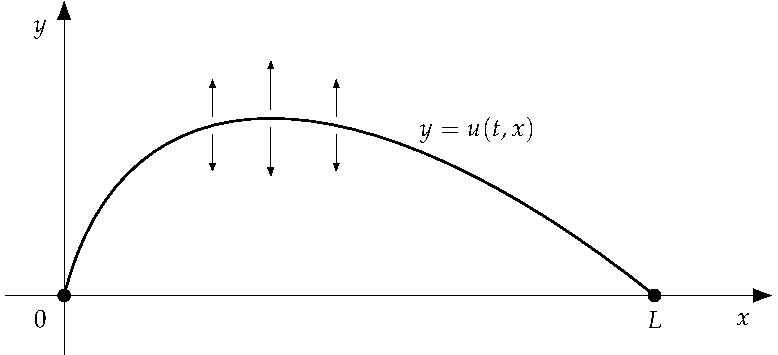
\includegraphics{tikz_string.pdf}
  \caption{Representation of the stretched string system. The arrows represent the
  transverse motion of the string.}
  \label{fig:string}
\end{figure}
%%%%%%%%%%%%%%%%%%%%%%%%%%%%%%%%%%%%%%%%%%%%%%%%%%%%%%%%%%%%%%%%%%%%%%%%%%%%%%%%%%%%%%%%%%
\section{Derivation of the wave equation}
Let us apply the laws of mechanics to derive an equation describing the dynamics of this
system. We first start by approximating the string by a large number $N$ of elastic line
segments of equal mass $\epsilon\mu$, with $\epsilon=\frac{L}{N}$. The $n$-th segment on
the string has the end points $P_n=(x_n,y_n)$ and $P_{n+1}=(x_{n+1},y_{n+1})$, starting
from $P_0=(0,0)$ up to $P_N=(L,0)$. The continuous string dynamics will then be later
obtained through the $N\to+\infty$ limit, or equivalently $\epsilon\to 0$. We additionally
assume that each segment respond to the same tension $T$ at its end points. A view of the
vicinity of $n$-th segment is represented in~\cref{fig:string-inf}. We define the angle
$\theta_n$ between the $n$-th segment and the $x$-axis. At the point $P_n$, the total
force $\vec{F}_n$ is given by the tension forces from the neighbouring segments on the
string, explicitly
\begin{equation}
  \vec{F}_n=\vec{T}_n^-+\vec{T}_n^+\,,\label{eq:string-force}
\end{equation}
where the vectors $\vec{T}_n^\pm$ both have magnitude $T$ and are represented by the blue
arrows in~\cref{fig:string-inf}. Using the angles $\theta_n$ previously defined, the
coordinates of the tension forces are given by
\begin{align}
  \vec{T}_n^-&=-T(\cos(\theta_{n-1}),\sin(\theta_{n-1}))\,,\label{eq:stringtm}\\
  \vec{T}_n^+&=T(\cos(\theta_{n}),\sin(\theta_{n}))\,.\label{eq:stringtp}
\end{align}
Using Pythagoras' theorem and elementary trigonometry, one can write
\begin{align}
  \cos(\theta_n)&=\frac{x_{n+1}-x_n}{\sqrt{(x_{n+1}-x_n)^2+(y_{n+1}-y_n)^2}}\,,\\
  \sin(\theta_n)&=\frac{y_{n+1}-y_n}{\sqrt{(x_{n+1}-x_n)^2+(y_{n+1}-y_n)^2}}\,.
\end{align}
Defining the ratio $d_n=\smash{\frac{y_{n+1}-y_n}{x_{n+1}-x_n}}$, the expressions above
can be further simplified to
\begin{equation}
  \cos(\theta_n)=\frac{1}{\sqrt{1+d_n^2}}\qquad\text{and}\qquad
  \sin(\theta_n)=\frac{d_n}{\sqrt{1+d_n^2}}\,.\label{eq:csthetan}
\end{equation}
Now, using Newton's Second Law with the total force~\cref{eq:string-force}, one obtains
the following system of differential of equations for the motion of $P_n$:
\begin{align}
  \epsilon\mu \frac{\diff^2 x_n}{\diff t^2}&=
  T\left(\frac{1}{\sqrt{1+d_{\smash{n}}^2}}-\frac{1}{\sqrt{1+d_{\smash{n-1}}^2}}\right)\,,
  \label{eq:string-fullxeq}\\
  \epsilon\mu \frac{\diff^2 y_n}{\diff t^2}&=
  T\left(\frac{d_n}{\sqrt{1+d_{\smash{n}}^2}}-\frac{d_{\smash{n-1}}}{\sqrt{1+d_{\smash{n-1}}^2}}\right)\,.
  \label{eq:string-fullyeq}
\end{align}
This is a rather non-trivial system of coupled non-linear differential equations, and we
will now use our small amplitude assumption to simplify it. This approximation means that
the vertical distances $y_{n+1}-y_n$ are expected to be much smaller than the horizontal
ones $x_{n+1}-x_n$, or in other words, $d_n$ is close to zero. Let us then
expand~\cref{eq:string-fullxeq,eq:string-fullyeq} for $d_n\to 0$. We first remind the
Taylor expansion
\begin{equation}
  \frac{1}{\sqrt{1+x^2}}=1-\frac{x^2}{2}+\mathcal{O}(x^4)\,,
\end{equation}
leading to the leading-order approximation
\begin{align}
  \frac{\diff^2 x_n}{\diff t^2}&=0\,,\label{eq:string-loxeq}\\
  \frac{\diff^2 y_n}{\diff t^2}&=\frac{T}{\epsilon\mu}(d_{n}-d_{n-1})\,,\label{eq:string-loyeq}
\end{align}
which is valid up to $\mathcal{O}(d_n^2)$ corrections. One remarkable feature of this
system is the fact that there is no force applying in the $x$ direction at leading order.
Since we assumed the string to be attached at its end points, this implies that there is
no motion in the $x$ direction. Oscillations in the $x$ and $y$ directions are called
\emph{longitudinal} and \emph{transverse} oscillations, respectively. We just obtained a
well-known result for string oscillations: in the limit of small oscillations, only
transverse oscillations are present.
\begin{figure}[t]
  \centering
  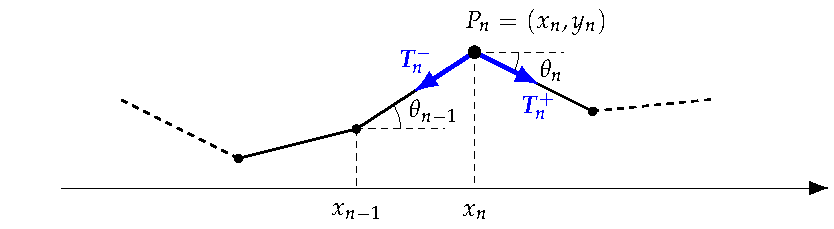
\includegraphics{tikz_string-inf.pdf}
  \caption{Discrete view of the string geometry and forces. The blue arrows represent the
  individual tension forces at point $P_n$.}
  \label{fig:string-inf}
\end{figure}

With the observation above, we can now exclusively focus on solving the transverse
equation of motion~\cref{eq:string-loyeq}. We assumed the string to have a uniform mass
distribution, and since the $x_n$ coordinates are constant and divide the string in
segments of equal mass, for all $n$ one has
\begin{equation}
  x_{n+1}-x_n=\epsilon\,.
\end{equation}
We additionally define the coordinates $y_n$ to be represented by a smooth function $u$ of
$x_n$ and the time $t$:
\begin{equation}
  y_n=u(t,x_n)\,.
\end{equation}
Substituting the equations above in~\cref{eq:string-loyeq}, one obtains
\begin{equation}
  \pdn{u}{t}{2}(t,x_n)=\frac{T}{\epsilon^2\mu}
  [u(t,x_{n}+\epsilon)-2u(t,x_{n})+u(t,x_{n}-\epsilon)]\,.\label{eq:wave-eq-discrete}
\end{equation}
We are now ready to obtain the continuous string equation by taking the $\epsilon\to 0$
limit. One starts by writing the Taylor expansion
\begin{equation}
  u(t,x+\epsilon)=u(t,x)+\epsilon\,\pd{u}{x}(t,x)
  +\frac{\epsilon^2}{2}\pdn{u}{x}{2}(t,x)+\mathcal{O}(\epsilon^3)\,,
\end{equation}
which implies that
\begin{equation}
  \lim_{\epsilon\to 0}=\frac{1}{\epsilon^2}
  [u(t,x+\epsilon)-2u(t,x)+u(t,x-\epsilon)]=\pdn{u}{x}{2}(t,x)\,.
\end{equation}
Using this last step with~\cref{eq:wave-eq-discrete} leads us to the main result of this
section, the \emph{wave equation}
\begin{equation}
  \boxed{
    \pdn{u}{t}{2}=c^2\,\pdn{u}{x}{2}
    \qquad\text{with}\qquad
  c=\sqrt{\frac{T}{\mu}}\,.}
  \label{eq:wave-eq}
\end{equation}
The parameter $c$, which has dimensions $\mathrm{L}\mathrm{T}^{-1}$, is usually called the
\emph{wave speed} for reasons that will be clear later in this section. The wave equation
is a homogeneous second-order partial differential equation, and will now discuss how to
solve it for the plucked string problem.
%%%%%%%%%%%%%%%%%%%%%%%%%%%%%%%%%%%%%%%%%%%%%%%%%%%%%%%%%%%%%%%%%%%%%%%%%%%%%%%%%%%%%%%%%%
\section{Travelling wave solutions}
\label{sec:wave-eq-travelling}
\subsection{General solutions}
We will first derive the general form of the solutions of the wave
equation~\cref{eq:wave-eq}. This derivation was first written by Jean le Rond d'Alembert
in 1747. \cref{eq:wave-eq} can be rewritten as follows
\begin{equation}
  \left(\pdn{}{t}{2}-c^2\,\pdn{}{x}{2}\right)u=
  \left(\pd{}{t}-c\,\pd{}{x}\right)
  \left(\pd{}{t}+c\,\pd{}{t}\right)u=0\,,
  \label{eq:wave-eq-factor}
\end{equation}
which is the composition of two first order derivatives. From this form, we would like to
define new length variables $\eta$ and $\xi$ such that
\begin{align}
  c\pd{}{\eta}&=\pd{}{t}+c\,\pd{}{x}\,,\\
  c\pd{}{\xi}&=\pd{}{t}-c\,\pd{}{x}\,.
\end{align}
Using the chain rule, we know that
\begin{align}
  \pd{}{\eta}&=\pd{t}{\eta}\pd{}{t}+\pd{x}{\eta}\pd{}{x}\,,\\
  \pd{}{\xi}&=\pd{t}{\xi}\pd{}{t}+\pd{x}{\xi}\pd{}{x}\,\,,
\end{align}
which implies that
\begin{equation}
  \pd{t}{\eta}=\frac{1}{c},\qquad\pd{x}{\eta}=1,\qquad
  \pd{t}{\xi}=\frac{1}{c},\qquad\text{and}\qquad\pd{x}{\xi}=-1\,.
\end{equation}
It is now clear that
\begin{align}
  t&=\frac{1}{c}(\eta+\xi)\,,\\
  x&=\eta-\xi\,,
\end{align}
is a possible solution, which can be inverted to
\begin{align}
  \eta&=x+ct\,,\\
  \xi&=x-ct\,.
\end{align}
In these new variables, the wave equation~\cref{eq:wave-eq-factor} becomes
\begin{equation}
  \frac{\partial^2 u}{\partial\eta\partial\xi}=0\,.
\end{equation}
In this simpler form, we can integrate the two derivatives sequentially. Starting with the
derivative in $\eta$, the right-hand side of the equation being zero means that
$\smash{\pd{u}{\xi}}$ is a constant in $\eta$. However, this constant can vary for any
value of $\xi$. In other words, there exists a function of one variable $\phi$ such that
\begin{equation}
  \pd{}{\xi}u(\eta,\xi)=\phi(\xi)\,.
\end{equation}
Following the same logic, as a function of $\xi$, $u$ is therefore an antiderivative of
$\phi$ up to a constant, which can vary with $\eta$. Therefore, there exists two functions
of a single variable $f$ and $g$ such that
\begin{equation}
  u(\eta,\xi)=f(\xi)+g(\eta)\,,
\end{equation}
where here $f$ is such that $f'=\phi$. In conclusion, switching back to the original
variables $x$ and $t$, the general solutions of the wave equation have the form
\begin{equation}
  \boxed{u(t,x)=f(x-ct)+g(x+ct)\,,}\label{eq:wave-eq-sol}
\end{equation}
where $f$ and $g$ can be any twice-differentiable functions. $f$ and $g$ are called the
\emph{forward-travelling} and \emph{backward-travelling} wave functions, respectively.
These functions are named in this way for the following reason. At $t=0$, if one pick a
point on the curve of $f$ with $x$-coordinate $x_0$, then at an arbitrary time $t$ the
same point will have the $x$-coordinate
\begin{equation}
  x(t)=x_0+ct\,,
\end{equation}
\ie it is moving forward on the $x$ axis. Also, one notices that $\td{x}{t}=c$, meaning
the point is moving with speed $c$, justifying the name \emph{wave speed} introduced
earlier. The same observation can be made for $g$, moving backward on the $x$ axis.

As we can see, the space of solutions of the wave equation is very large as both forward
and backward contribution are arbitrary functions. However, it is known, and will be
admitted here, that the wave equation has a unique solution if one impose the two initial
conditions
\begin{equation}
  u_0(x)=u(0,x)\qquad\text{and}\qquad u_1(x)=\pd{u}{t}(0,x)\,,\label{eq:wave-eq-ic}
\end{equation}
which physically represent the initial position of the string and its initial velocity,
respectively. With this in mind, we will now discuss the solution of the wave equations
specifically for the plucked string problem.
%
\subsection{Particular solutions of the plucked string problem}
We remind here the considered physical problem: the string will be pulled in a given
position, and then released. This means the initial velocity $u_1$ in~\cref{eq:wave-eq-ic}
is zero. Additionally, the string is attached at the two points $(0,0)$ and $(L,0)$, which
implies that for all times $t\in\mathbb{R}$
\begin{equation}
  u(t,0)=0\qquad\text{and}\qquad u(t,L)=0\,.\label{eq:string-bc}
\end{equation}
These constraints are called the \emph{boundary conditions} of the wave equation, and they
generally have a strong influence on the set of solutions. We now show how initial
conditions and boundary conditions determine a unique solution to the wave equation.

Applying both initial conditions in~\cref{eq:wave-eq-ic} to the general wave equation
solutions~\cref{eq:wave-eq-sol}, one obtains for all $x\in[0,L]$
\begin{align}
  f(x)+g(x)&=u_0(x)\label{eq:wave-eq-fpg}\,,\\
  g'(x)-f'(x)&=0\,.
\end{align}
The second equation above implies that there exists a constant $K$ such that for all
$x\in[0,L]$,
\begin{equation}
  f(x)=g(x)+\frac{K}{2}\,,\label{eq:wave-eq-fmg}
\end{equation}
where the arbitrary factor $\frac12$ is introduced for later convenience.
Solving~\cref{eq:wave-eq-fpg,eq:wave-eq-fmg} as a linear system, one obtains, for all
$x\in[0,L]$,
\begin{align}
  f(x)&=\frac{1}{2}u_0(x)+K\,,\label{eq:wave-eq-f0L}\\
  g(x)&=\frac{1}{2}u_0(x)-K\,.\label{eq:wave-eq-g0L}
\end{align}
In summary, we found that the initial conditions imply that, on the interval $[0,L]$, $f$
and $g$ are both equal to half the initial position $u_0$, up to an integration constant.

To obtain the full solution~\cref{eq:wave-eq-sol}, we now need to solve $f$ and $g$
outside the interval $[0,L]$, which can be done using the boundary
conditions~\cref{eq:string-bc}. The first boundary condition implies that for all
$t\in\mathbb{R}$,
\begin{equation}
  f(-ct)=-g(ct)\,.
\end{equation}
Using~\cref{eq:wave-eq-f0L,eq:wave-eq-g0L}, the equation above allows us to solve $f$ and
$g$ on the interval $[-L,0]$, \ie for all $x\in[0,L]$
\begin{align}
  f(-x)&=-\frac{1}{2}u_0(x)+K\,,\label{eq:wave-eq-fmL0}\\
  g(-x)&=-\frac{1}{2}u_0(x)-K\,.\label{eq:wave-eq-gmL0}
\end{align}
Now, the second boundary condition in~\cref{eq:string-bc} implies that for all
$t\in\mathbb{R}$,
\begin{equation}
  f(L-ct)=-g(L+ct)=f(-L-ct)\,.
\end{equation}
For all $x\in\mathbb{R}$, the equation above for $t=-\frac{1}{c}(L+x)$ gives
\begin{equation}
  f(x+2L)=f(x)\,.
\end{equation}
This last equation means that $f$ is periodic with period $\lambda=2L$, called the
\emph{wavelength} of the vibration. The same can be identically shown for $g$. This
implies that for any integer $n$, $f$ and $g$ on the translated interval $[-L+2nL,L+2nL]$
take the same values as on $[-L,L]$. Since~\cref{eq:wave-eq-f0L,eq:wave-eq-g0L},
and~\cref{eq:wave-eq-fmL0,eq:wave-eq-gmL0} define $f$ and $g$ on $[-L,L]$, we have
completely solved the wave equation.

Let us summarise the solution derived above. First we can observe
through~\cref{eq:wave-eq-f0L,eq:wave-eq-g0L}, and~\cref{eq:wave-eq-fmL0,eq:wave-eq-gmL0}
that the constant $K$ will always cancel when summing $f$ and $g$ to obtain $u$.
Therefore, we can assume without loss of generality that $K=0$, which implies that $f=g$.
Finally, the solution of the wave equation for the plucked string problem if given by
\begin{equation}
  u(t,x)=f(x-ct)+f(x+ct)\,,\label{eq:string-sol}
\end{equation}
with
\begin{equation}
  f(x)=
  \begin{cases}
    u_0(x-2nL)&~\text{if}\quad2nL\leq x\leq (2n+1) L\\
    -u_0(2nL-x)&~\text{if}\quad(2n-1)L\leq x\leq 2nL
  \end{cases}
  \,,\label{eq:f-copies}
\end{equation}
where $n$ is any integer, and $u_0(x)$ is the initial string position. One important
observation can be made: since $f$ is periodic with period $\lambda$, it implies
using~\cref{eq:string-sol} that $u(t,x)$ is also periodic in time with period
\begin{equation}
  \tau=\frac{\lambda}{c}\,.
\end{equation}
Now, defining the \emph{frequency} $\smash{\omega=\frac{1}{\tau}}$, and reminding the
definition of $c$ from~\cref{eq:wave-eq}, we obtain
\begin{equation}
  \boxed{\omega=\frac{c}{\lambda}=\frac{1}{2L}\sqrt{\frac{T}{\mu}}}\,.
  \label{eq:mersenne-law}
\end{equation}
This result is called \emph{Mersenne's law}, and predicts the vibration frequency of a
string as a function of its length, tension, and linear mass density.

\begin{figure}[t]
  \centering
  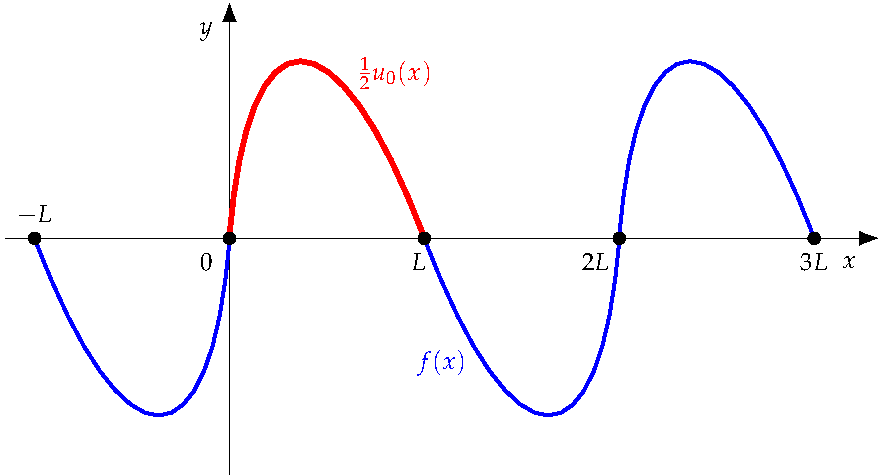
\includegraphics{tikz_string-f.pdf}
  \caption{Graphical representation of~\cref{eq:f-copies}. The bold red line represents
    the initial string position $u_0(x)$. The blue line is the forward component $f(x)$,
  obtained as the periodic extension of $u_0(x)$ defined in~\cref{eq:f-copies}.}
  \label{fig:string-f}
\end{figure}
\begin{figure}[t]
  \centering
  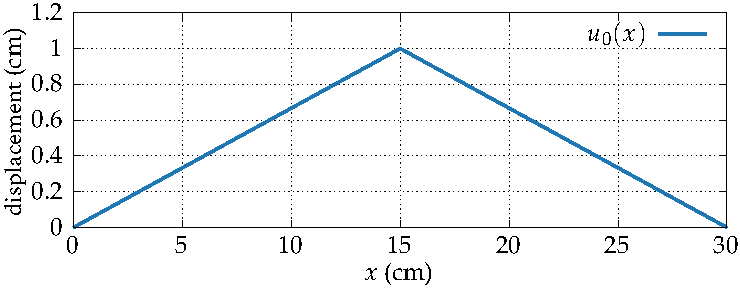
\includegraphics{gp_string-pulled.pdf}\\
  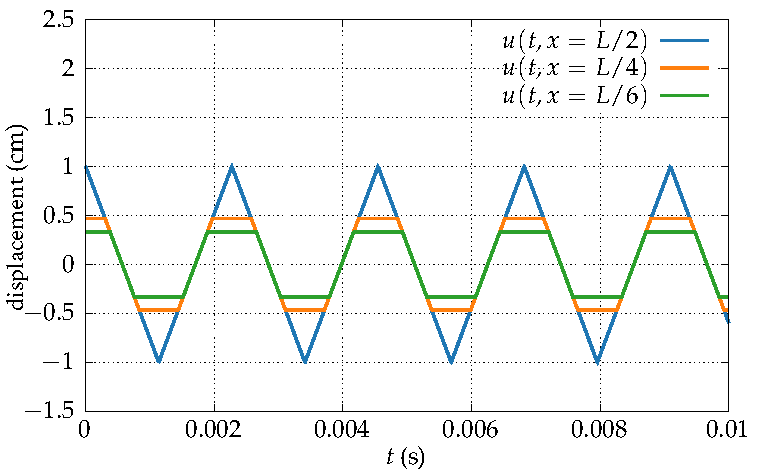
\includegraphics{gp_string-pulled-time.pdf}
  \caption{Initial condition~\cref{eq:string-pluck-ic} (upper pane) and resulting
    oscillations in time at various positions on the string (lower pane) with
    $A=\unit{1}{\centi\metre}$, $L=\unit{30}{\centi\metre}$, $T=\unit{63.4}{\newton}$, and
  $\mu=\unit{0.91}{\gram\per\metre}$.}
  \label{fig:string-pulled}
\end{figure}
We conclude this section by a slightly more practical discussion of the structure of the
solution. \cref{eq:f-copies} is somewhat abstract, but all it means is that the curve of
$f$ is constructed by sequentially repeating the curve of $u_0(x)$, rotating it by
$180^{\circ}$ at each iteration. This construction is illustrated in~\cref{fig:string-f}.
%
\subsection{Explicit example}
Let us now look at an explicit solution. We assume that initially the string middle point
is pulled to a distance $A$ from the $x$-axis, and that it is perfectly straight between
this point and its extremities. Explicitly, this can be parameterised by the following
initial condition
\begin{equation}
  u_0(x)=
  \begin{cases}
    \frac{2A}{L}x&~\text{if}\quad 0\leq x \leq \frac{L}{2}\\
    \frac{2A}{L}(L-x)&~\text{if}\quad \frac{L}{2}\leq x \leq L
  \end{cases}\,,
  \label{eq:string-pluck-ic}
\end{equation}
represented in the upper pane of~\cref{fig:string-pulled}. Let us give explicit values for
the all the parameters of the problem. We assume the string length $L$ is
$\unit{30}{\centi\metre}$, its linear mass density $\mu$ is
$\unit{0.91}{\gram\per\metre}$, and it is stretched to a tension $T$ of
$\unit{63.4}{\newton}$. We additionally assume the pulling distance $A$ to be
$\unit{1}{\centi\metre}$. Let us start by using~\cref{eq:wave-eq} to compute the wave
speed $c$
\begin{equation}
  c=\sqrt{\frac{T}{\mu}}
  =\sqrt{\frac{\unit{63.4}{\newton}}{\unit{0.91\times 10^{-3}}{\kilo\gram\per\metre}}}
  =\unit{263.95}{\metre\per\second}\,.
\end{equation}
Then, using Mersenne's law~\cref{eq:mersenne-law} with the wavelength
$\lambda=2L=\unit{60}{\centi\metre}$, we can compute the frequency of the string
vibration:
\begin{equation}
  \omega=\frac{c}{\lambda}=\frac{\unit{263.95}{\metre\per\second}}{\unit{0.6}{\metre}}
  =\unit{439.92}{\hertz}.
\end{equation}
So this string is approximately tuned to give the standard musical pitch $\mathrm{A}_4$ at
the $\unit{440}{\hertz}$ frequency. Explicit plots of the string vibrations at different
positions on the string are given in the lower pane of~\cref{fig:string-pulled}.
%%%%%%%%%%%%%%%%%%%%%%%%%%%%%%%%%%%%%%%%%%%%%%%%%%%%%%%%%%%%%%%%%%%%%%%%%%%%%%%%%%%%%%%%%%
\section{Standing wave solutions}
The previous steps entirely solved the wave equation for the problem we are interested in.
However, there is another way to solve this equation which is going to be very relevant
for what follows. Let us come back to~\cref{fig:string-f} and how the wave equation
forward wave function $f$ is built as a periodic extension of the initial condition. One
can notice how the symmetries of $f$, \ie it is periodic and odd, are identical to those
of the sine function. In fact, the structure of $f$ implies that if we would initially
pull the string into a position which is exactly half a period of the sine function, \ie
\begin{equation}
  \forall x\in[0,L],\quad u_0(x)=A\sin\left(\frac{\pi}{L}x\right)\,,\label{eq:string-sine-ic}
\end{equation}
then the extension~\cref{eq:f-copies} of $u_0$ to $f$ is defined by the same formula, \ie
$f(x)=\smash{A\sin\left(\frac{\pi}{L}x\right)}$ for any real number $x$, and the solution
to the wave equation is simply
\begin{equation}
  u(t,x)=\frac{A}{2}\left\{\sin\left[\frac{\pi}{L}(x+ct)\right]
  +\sin\left[\frac{\pi}{L}(x-ct)\right]\right\}\,.
\end{equation}
The choice~\cref{eq:string-sine-ic} is not unique, all is needed for the sine function is
to take the value zero at $x=0$ and $x=L$, which can generally be obtained with
\begin{equation}
  u_0(x)=A\sin\left(\frac{\pi}{L}nx\right)\,,
\end{equation}
where $n$ is an arbitrary integer, and the associated solution is
\begin{equation}
  u(t,x)=\frac{A}{2}\left\{\sin\left[\frac{\pi}{L}n(x+ct)\right]
  +\sin\left[\frac{\pi}{L}n(x-ct)\right]\right\}\,.
  \label{eq:stand-wave-travel}
\end{equation}
Now, using the trigonometric identities
\begin{align}
  \sin(a+b)&=\sin(a)\cos(b)+\cos(a)\sin(b)\,,\\
  \sin(a-b)&=\sin(a)\cos(b)-\cos(a)\sin(b)\,,
\end{align}
$u(t,x)$ can be simplified to
\begin{equation}
  u(t,x)=A\sin\left(\frac{\pi}{L}nx\right)\cos\left(\frac{\pi}{L}nct\right)
  =\cos\left(\frac{\pi}{L}nct\right)f(x)\,.
  \label{eq:stand-wave-example}
\end{equation}
In this particular solution, time and space oscillations factorise and the wave function
$f$ does not ``travel'' any more. Such solution is called a \emph{standing wave solution}
of the wave equation. At this stage, this might just look like a special set of particular
solutions built on the symmetries of $f$. However, as we will see in this course, those
are of extreme importance for describing oscillatory phenomena, and were historically a
crucial part of the work of Jean-Baptiste Joseph Fourier (early 19\textsuperscript{th}
century), which led to the so-called Fourier analysis theory.

For now, let us question the generality of the standing wave solution above. To do that,
we start by considering a general standing wave solution of the wave equation:
\begin{equation}
  u(t,x)=F(t)G(x)\,.
\end{equation}
Applying the wave equation~\cref{eq:wave-eq}, one obtains
\begin{equation}
  \left(\pdn{}{t}{2}-c^2\,\pdn{}{x}{2}\right)u(t,x)=F''(t)G(x)-c^2F(t)G''(x)=0\,,
\end{equation}
which implies that
\begin{equation}
  \frac{F''(t)}{F(t)}=c^2\frac{G''(x)}{G(x)}\,.\label{eq:sep-var}
\end{equation}
The left-hand side of this equation only depends on $t$, and the right-hand side only
depends on $x$. This is typical of standing wave solution, and looking for such
simplification is sometime referred as the \emph{separation of variables} method. A key
observation is that~\cref{eq:sep-var} implies that there exists a constant $\alpha$ such
that
\begin{equation}
  \frac{1}{c^2}\frac{F''(t)}{F(t)}=\frac{G''(x)}{G(x)}=\alpha\,.
\end{equation}
Indeed, since this expression can be written solely as a function of $x$ or $t$, it means
that both its partial derivatives in $x$ and $t$ vanish, implying that it is a constant
function of $x$ and $t$. With that established, the equation above can be rewritten as the
following system of ordinary differential equations
\begin{align}
  F''(t)&=c^2\alpha F(t)\,,\label{eq:sep-var-F}\\
  G''(x)&=\alpha G(x)\,.
\end{align}
We can solve these equations using the \emph{characteristic equation method}. Let us start
with the equation for $G$. We try to look for particular solutions of the form
\begin{equation}
  G(x)=e^{rt}\,,
\end{equation}
which would imply that
\begin{equation}
  G''(x)=r^2e^{rx}=\alpha e^{rx}\,,
\end{equation}
and therefore for such solution to exists $A$ must be a solution of the characteristic
equation
\begin{equation}
  r^2-\alpha=0\,.
\end{equation}
At this stage $\alpha$ is an arbitrary real number, and depending on its sign the equation
above can have the different solutions. For convenience let us define
$\beta=\smash{\sqrt{|\alpha|}}$, we have the following cases
\begin{enumerate}
  \item $\alpha>0$: then $r$ is a real number equal to $\pm \beta$, the particular
    solutions for $G(x)$ are $\smash{e^{\beta x}}$ and $\smash{e^{-\beta x}}$, and the
    general solutions are the linear combinations $G(x)=a\smash{e^{\beta
    x}}+b\smash{e^{-\beta x}}$ for any real numbers $a$ and $b$.
  \item $\alpha<0$: then $r$ is a purely imaginary complex number equal to $\pm i\beta$,
    the particular solutions for $G(x)$ are $\smash{e^{i\beta x}}$ and $\smash{e^{-i\beta
    x}}$, and the general solutions are the linear combinations $G(x)=a\smash{e^{i\beta
    x}}+b\smash{e^{-i\beta x}}$ for any complex numbers $a$ and $b$. Since $G$ is a real
    function, it has to verify the identity $G^*=G$, where $G^*$ is the complex conjugate
    of $G$. This implies that $a^*=b$.

  \item $\alpha=0$: then $A=0$ and $G(x)=1$. Additionally, in that case the equation for
    $G$ becomes $G''(x)=0$, which simply means that $G$ is a linear function of the form
    $G(x)=ax+b$.
\end{enumerate}
To discriminate between all these cases, let us consider the boundary
conditions~\cref{eq:string-bc}, which immediately implies that
\begin{equation}
  G(0)=0\qquad\text{and}\qquad G(L)=0\,.
\end{equation}
Clearly, in cases 1.~and 3.~above, the only possible solutions satisfying these conditions
would be with $a=b=0$ and therefore $G(x)=0$ and $u(t,x)=0$. This is the trivial solution
of an immobile string at equilibrium. In case 2., we write $a=\smash{C_1+iC_2}$ where
$\smash{C_1}=\Re(a)$ and $\smash{C_2}=\Im(a)$ are the real and imaginary parts of $a$,
respectively, and then the general solution for $G(x)$ can be written
\begin{equation}
  G(x)=ae^{i\beta x}+(ae^{i\beta x})^*=2\Re(ae^{i\beta x})=C_1\cos(\beta x)-C_2\sin(\beta x)\,.
\end{equation}
Now, the boundary condition $G(0)=0$ immediately gives $C_1=0$, and $G(L)=0$ implies
\begin{equation}
  \sin(\beta L)=0\,,
\end{equation}
which means that there exist an integer $n$ such that
\begin{equation}
  \beta=\frac{\pi}{L}n\,,
\end{equation}
and finally
\begin{equation}
  G(x)=-C_2\sin\left(\frac{\pi}{L}nx\right)\,.
\end{equation}
We know turn to the time component $F$ determined by the equation~\cref{eq:sep-var-F}. The
constant $\alpha$ in this equation is identical and was already strongly constrained while
solving for $G$. Following the same steps as above, up to an additional factor of $c^2$,
we find that
\begin{equation}
  F(t)=D_1\cos\left(\frac{\pi}{L}nc t\right)-D_2\sin\left(\frac{\pi}{L}nc t\right)\,,
\end{equation}
with two unknown real constants $D_1$ and $D_2$. We know use the second initial condition
in~\cref{eq:wave-eq-ic} which implies that $F'(0)=0$. The derivative of $F$ is given by
\begin{equation}
  F'(t)=-\frac{\pi}{L}ncD_1\sin\left(\frac{\pi}{L}nc t\right)-\frac{\pi}{L}ncD_2
  \cos\left(\frac{\pi}{L}nc t\right)\,,
\end{equation}
and $F'(0)=0$ implies that $D_2=0$. Putting everything together, we get the solution
\begin{equation}
  u(t,x)=A\sin\left(\frac{\pi}{L}nx\right)\cos\left(\frac{\pi}{L}nct\right)\,,
\end{equation}
with $A=-C_2D_1$. We can observe this is the same result as~\cref{eq:stand-wave-example}.
This is a non-trivial and very important result: although we originally found the standing
wave solutions above as a simple example, we just proved that \emph{all} standing wave
solutions can be written in that way. However, the standing wave solutions have fairly
unrealistic initial conditions where the string needs starts exactly shaped as a portion
of the sine function curve. One legitimate question is whether these solutions are just
exceptional solutions, or can they be related to the general solutions discussed
in~\cref{sec:wave-eq-travelling}? One could argue that answering this question is the core
topic of this course. We will now conclude this chapter by inferring a possible answer to
that question.
%%%%%%%%%%%%%%%%%%%%%%%%%%%%%%%%%%%%%%%%%%%%%%%%%%%%%%%%%%%%%%%%%%%%%%%%%%%%%%%%%%%%%%%%%%
\section{Towards Fourier series}
\label{sec:toward-fourier}
A key property of the wave equation~\cref{eq:wave-eq} is that it is linear. It means that
if $u(t,x)$ and $v(t,x)$ are two solutions of the equation, then clearly for any real
numbers $\alpha$ and $\beta$, the linear combination
\begin{equation}
  w(t,x)=\alpha u(t,x)+\beta v(t,x)\,,
\end{equation}
is also clearly a solution of the equation. Let us consider the set of all possible
standing wave solutions
\begin{equation}
  s_n(t,x)=A_n\sin\left(\frac{\pi}{L}nx\right)\cos\left(\frac{\pi}{L}nct\right)\,,
\end{equation}
where $n$ is any integer and $A_n$ is a real number depending on $n$. First, we can
observe that
\begin{equation}
  s_{-n}(t,x)=-s_n(t,x)\,,
\end{equation}
and in particular $s_0=0$. So in the rest of this section we will assume, without loss of
generality, that $n>0$. Then by linearity the series
\begin{equation}
  u(t,x)=\sumnp{n}s_n(t,x)\,,
\end{equation}
which, for the moment, we assume to be convergent, is a solution of the wave equation. The
question raised at the end of the previous question can then be reformulated as: for a
given initial string position $u_0(x)$, is there a sequence of real numbers $A_n$ such
that the solution of the wave equation can be expressed as the superposition of standing
waves above? Explicitly, this would imply that
\begin{equation}
  \label{eq:string-ic-fourier}
  u_0(x)=u(0,x)=\sumnp{n}s_n(0,x)=\sumnp{n}A_n\sin\left(\frac{\pi}{L}nx\right)\,.
\end{equation}
To try determining $A_n$, a key identity is
\begin{equation}
  \int_{0}^{L}\diff x\,\sin\left(\frac{\pi}{L}nx\right)\sin\left(\frac{\pi}{L}mx\right)
  =
  \begin{cases}
    0&~\text{if}\quad n\neq m\\
    \frac{L}{2}&~\text{if}\quad n=m
  \end{cases}
  \,,
\end{equation}
for all pairs of positive integers $n$ and $m$. We will admit this identity for now, it
will be proven in the next chapter. This formula implies that
\begin{equation}
  \frac{2}{L}\int_{0}^{L}\diff x\, u_0(x)\sin\left(\frac{\pi}{L}nx\right)=A_n\,,
\end{equation}
providing a direct way to compute the coefficients $A_n$, and once again we assumed that
the series convergence is well-behaved enough to allow commuting the sum and the integral.
We can try to use this formula with the plucked string initial condition
in~\cref{eq:string-pluck-ic} and~\cref{fig:string-pulled}. We start by considering the
first half of the string
\begin{align}
  \frac{2}{L}\int_{0}^{\frac{L}{2}}\diff x\, u_0(x)\sin\left(\frac{\pi}{L}nx\right)&
  =\frac{4A}{L^2}\int_{0}^{\frac{L}{2}}\diff x\, x\sin\left(\frac{\pi}{L}nx\right)\\
  \label{eq:string-pluck-fourier1}
  &=-\frac{4A}{\pi n L}\left[x\cos\left(\frac{\pi}{L}nx\right)\right]_0^{\frac{L}{2}}
  +\frac{4A}{\pi n L}\int_{0}^{\frac{L}{2}}\diff x\,\cos\left(\frac{\pi}{L}nx\right)\\
  \label{eq:string-pluck-fourier2}
  &=-\frac{2A}{\pi n}\cos\left(\frac{\pi}{2}n\right)+\frac{4A}{\pi^2 n^2}
  \left[\sin\left(\frac{\pi}{L}nx\right)\right]_0^{\frac{L}{2}}\\
  &=-\frac{2A}{\pi n}\cos\left(\frac{\pi}{2}n\right)+\frac{4A}{\pi^2 n^2}
  \sin\left(\frac{\pi}{2}n\right)\,,
\end{align}
where integration by parts was used to go from~\cref{eq:string-pluck-fourier1}
to~\cref{eq:string-pluck-fourier2}. Using the same procedure,
\begin{align}
  \frac{2}{L}\int_{\frac{L}{2}}^{L}\diff x\, u_0(x)\sin\left(\frac{\pi}{L}nx\right)
  &=\frac{4A}{L^2}\int_{\frac{L}{2}}^{L}\diff x\, (L-x)\sin\left(\frac{\pi}{L}nx\right)\\
  &=\frac{2A}{\pi n}\cos\left(\frac{\pi}{2}n\right)+\frac{4A}{\pi^2 n^2}
  \sin\left(\frac{\pi}{2}n\right)\,.
\end{align}
Altogether, we obtain
\begin{equation}
  A_n=\frac{8A}{\pi^2 n^2}\sin\left(\frac{\pi}{2}n\right)
\end{equation}
Since $n$ is an integer, we know that
\begin{equation}
  \sin\left(\frac{\pi}{2}n\right)=
  \begin{cases}
    0&\text{if}~n~\text{is even}\\
    (-1)^{\frac{n-1}{2}}&\text{if}~n~\text{is odd}
  \end{cases}\,,\label{eq:sinpn2}
\end{equation}
and therefore $A_n=0$ if $n$ is even. In conclusion, only considering the odd
coefficients, the solution of the wave equation is
\begin{equation}
  u(t,x)=\frac{8A}{\pi^2}\sumnp{n}\frac{(-1)^n}{(2n+1)^2}
  \sin\left[\frac{\pi}{L}(2n+1)x\right]\cos\left[\frac{\pi}{L}(2n+1)ct\right]\,.
  \label{eq:string-fourier}
\end{equation}
This last equation is the same solution as~\cref{eq:string-sol}, but expressed purely in
terms of standing waves. This expression is called the \emph{Fourier series expansion} of
$u(t,x)$. In all this section, we made some rather strong assumptions on the convergence
of such series, and the generality of the procedure above is not clear at this stage. The
next two chapters will be dedicated to build a well-defined mathematical framework for
Fourier series.

We conclude this chapter with a couple of observations on the series above. Firstly, the
convergence of~\cref{eq:string-fourier} was assumed a priori, but it can be checked a
posteriori. Indeed, for all $n>0$ we have
\begin{equation}
  \left|\frac{(-1)^n}{(2n+1)^2}\sin\left[\frac{\pi}{L}(2n+1)x\right]
  \cos\left[\frac{\pi}{L}(2n+1)ct\right]\right|
  \leq\frac{1}{(2n+1)^2}\,.
\end{equation}
The right-hand side of this inequality is independent of $t$ and $x$, and the summand of a
convergent series, so~\cref{eq:string-sol} is an absolutely and uniformly convergent
series\footnote{More explicitly, this is a consequence of the Weierstrass $M$-test
theorem}. This does not prove that the series converges to $u(t,x)$, which we will not
discuss at this stage. However, that convergence can be observed at least numerically, as
illustrated in~\cref{fig:string-fourier}. Secondly, Fourier series generally allow
obtaining interesting series related to the number $\pi$. For example, here we know using
the initial condition~\cref{eq:string-pluck-ic} and the identity~\cref{eq:sinpn2} that
\begin{equation}
  u\left(0,\frac{L}{2}\right)=A=\frac{8A}{\pi^2}\sumnp{n}\frac{1}{(2n+1)^2}\,,
\end{equation}
giving us the remarkable identity
\begin{equation}
  \sumnp{n}\frac{1}{(2n+1)^2}=\frac{\pi^2}{8}\,,
  \label{eq:series-pi28}
\end{equation}
which elegantly connects $\pi$ and the sum of the inverse squares of all odd integers.
Interestingly, this somewhat accidental identity can be used to solve the Basel problem!
The Basel problem, originally solved by Leonhard Euler in 1734, consists in proving that
\begin{equation}
  \sumnp{n}\frac{1}{n^2}=\frac{\pi^2}{6}\,,
\end{equation}
which is a fundamental identity in number theory, as well as the $s=2$ value of the
Riemann zeta function. We note the series on the left-hand side as $\zeta$, and observe
that it is the sum of the inverse squares of all positive integers. Therefore, the
previously demonstrated identity~\cref{eq:series-pi28}, is a partial sum of $\zeta$
restricted to the odd integers. The missing contribution from even integers can be written
\begin{equation}
  \sumnp{n}\frac{1}{(2n)^2}=\frac{\zeta}{4}\,,
\end{equation}
and therefore
\begin{equation}
  \zeta=\sumnp{n}\frac{1}{(2n)^2}+\sumnp{n}\frac{1}{(2n+1)^2}
  =\frac{\zeta}{4}+\frac{\pi^2}{8}\,.
\end{equation}
Solving for $\zeta$ in the equation above, we obtain
\begin{equation}
  \zeta=\frac{\pi^2}{6}\,,
\end{equation}
which solves the Basel problem.
\begin{figure}
  \centering
  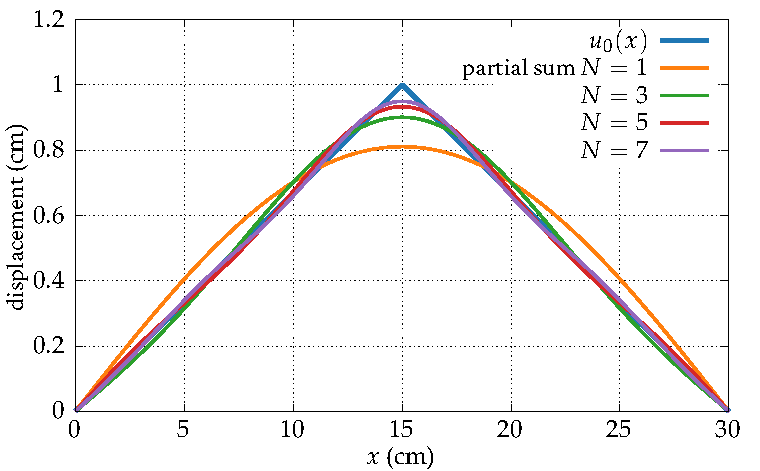
\includegraphics{gp_string-fourier.pdf}
  \caption{Initial condition $u_0(x)$~\cref{eq:string-pluck-ic}, compared to the partial
    sum $\sum_{n=1}^N A_n\sin(\frac{\pi}{L}nx)$ of the Fourier
  expansion~\cref{eq:string-ic-fourier}.}
  \label{fig:string-fourier}
\end{figure}

\vfill\pagebreak
% !TEX root = ../waves.tex
%%%%%%%%%%%%%%%%%%%%%%%%%%%%%%%%%%%%%%%%%%%%%%%%%%%%%%%%%%%%%%%%%%%%%%%%%%%%%%%%%%%%%%%%%%
\section{Exercises}
\begin{ExerciseList}
  %---------------------------------------------------------------------------------------
  \Exercise[label=odesincos] Let $f$ be a twice-differentiable real function on $\mathbb{R}$ which is
  a solution of the ordinary differential equation
  \begin{equation}
    f''(t) + A^2 f(t) = 0\,,
  \end{equation}
  where $A$ is a non-zero real number. We additionally define the functions $g$ and $h$
  with
  \begin{align}
    g(t)&=f(t)\cos(At)-\frac{f'(t)}{A}\sin(At)\label{eq:csgdef}\,,\\
    h(t)&=f(t)\sin(At)+\frac{f'(t)}{A}\cos(At)\label{eq:cshdef}\,.
  \end{align}
  \Question Show that $g$ and $h$ are constant functions.
  \Question Deduce from the previous question that there exists two real numbers $a$ and $b$
  such that
  \begin{equation}
    f(t)=a\cos(At)+b\sin(At)\,.\label{eq:csfsol}
  \end{equation}
  %---------------------------------------------------------------------------------------
  \Exercise[label=stringhooke] We start by recalling Hooke's law for the restoring force
  of a stretched or compressed spring. We assume a spring is aligned with the $x$-axis and
  has an equilibrium length of $\ell$. Hooke's law states that if the spring is stretched
  or compressed to a length $\ell+\delta\ell$, the tension forces at the extremities of
  the spring have a magnitude proportional to the displacement:
  \begin{equation}
    T=k|\delta\ell|\,,
  \end{equation}
  where $k$ is the \emph{spring constant} in $\newton\per\metre$. Additionally, if the
  spring is compressed, the forces are always directed towards the equilibrium position,
  \ie outward when the spring is compressed and inward when it is stretched. \Question
  From the point of view of Hooke's law, argue that the tension forces on the discretised
  string in~\cref{eq:stringtm,eq:stringtp} could be described in a more accurate way.
  \Question Use Hooke's law to generalise the equations of
  motion~\cref{eq:string-fullxeq,eq:string-fullyeq}.
  \Question Demonstrate that, assuming longitudinal movement is negligible, the
  generalisations above do not change the wave equation~\cref{eq:wave-eq} in the limit of
  small amplitudes.
  %---------------------------------------------------------------------------------------
  \Exercise[label=guitar] We consider a guitar string with a vibrating length
  $L=\unit{63}{\centi\metre}$ and a linear mass density $\mu=\unit{1.2}{\gram\per\metre}$.
  \Question What tension is required to apply to the string to tune it to the frequency
  $\unit{110}{\hertz}$? \Question Assuming the same tension as in Question 1, what is the
  wave speed on the string? \Question A finger is placed on the string at a distance
  $\ell$ from the nut (the extremity of the string farthest from the body), how is the
  string vibration frequency modified? \Question Assuming the same tension as in Question
  1, what finger position leads to a frequency of $\unit{164.81}{\hertz}$? \Question Frets
  on the fingerboard are spaced such that the frequency of the string increases by one
  halftone between two frets. A frequency $\omega'$ is one halftone higher than $\omega$
  if
  \begin{equation}
    \omega'=2^{\frac{1}{12}}\omega\,.
  \end{equation}
  Compute the distance from the nut of the first few frets.
  %---------------------------------------------------------------------------------------
  \InputIfFileExists{solutions/wave-eq}{}{}
\end{ExerciseList}

\shipoutAnswer
\chapter{Elementary waves}
\label{chap:elementary-waves}
% !TEX root = ../waves.tex
%%%%%%%%%%%%%%%%%%%%%%%%%%%%%%%%%%%%%%%%%%%%%%%%%%%%%%%%%%%%%%%%%%%%%%%%%%%%%%%%%%%%%%%%%%
\section{General properties of periodic functions}
A physical quantity $f(t)$ depending on a time variable $t$ is said to be
\emph{oscillating} or \emph{periodic} if it repeats itself identically after a certain
duration. In mathematical terms:
\begin{definition}
  A function $f$ of a single real variable is said to be~\emph{periodic} or specifically
  \emph{$\tau$-periodic} if there exists a positive real number $\tau$ such that
  \begin{equation}
    \forall t\in\mathbb{R},\quad f(t+\tau)=f(t)\,.
  \end{equation}
  $\tau$ is called a \emph{period} of $f$.
\end{definition}
\noindent For example, $\sin(t)$ is $2\pi$-periodic, and a constant function admits any
number has a period. Another fundamental quantity is the \emph{frequency}:
\begin{definition}
  If $\tau$ is a period of a given function $f$, its inverse
  \begin{equation}
    \omega=\frac{1}{\tau}
  \end{equation}
  is called a \emph{frequency} of $f$.
\end{definition}
\noindent In physical terms, if $t$ is a time variable, $\tau$ is also a time, and
$\omega$ is the number of oscillations per unit of time, generally given in Hertz
($\hertz$). One can notice that a periodic function never has a unique period, \eg clearly
if $\tau$ is a period, $2\tau$ is also a period. Because of this it is useful to write the
following definition
\begin{definition}
  The infimum $\tau_0$ of the set of all periods of a given periodic function $f$ is
  called the \emph{fundamental period} of $f$. The associated frequency
  $\omega_0=\frac{1}{\tau_0}$ is called the \emph{fundamental frequency} of $f$.
\end{definition}
\noindent For example, the fundamental frequency of $\sin(t)$ is $2\pi$, and it is zero
for a constant function. Another fundamental quantity is the \emph{amplitude} of a
periodic function, measuring the size of the oscillations within a fundamental period:
\begin{definition}
  \label{def:amplitude}
  Let $f$ be a real periodic function with fundamental period $\tau_0$. We additionally
  assume that $f$ is bounded with infimum and supremum
  \begin{equation}
    m=\inf_{0\leq t\leq \tau_0}f(t)\qquad\text{and}\qquad M=\sup_{0\leq t\leq \tau_0}f(t)\,.
  \end{equation}
  The \emph{amplitude} of $f$ is then defined by
  \begin{equation}
    A=\frac{M-m}{2}\,.
  \end{equation}
\end{definition}
\noindent For example, the amplitude of $\sin(t)$ is equal to $1$, and it is zero for
constant functions. \cref{def:amplitude} assumes that $f$ is bounded, and one can question
whether this hypothesis is true in general. It is not, but continuity is a sufficient
condition:
\begin{proposition}
  If a real periodic function is continuous, then it is bounded (and therefore it has a
  well-defined amplitude).
\end{proposition}
\begin{proof}
  Let $f$ be a continuous $\tau$-periodic function. Since $f$ is continuous on the compact
  interval $[0,\tau]$, it follows from the boundedness theorem that it is also bounded on
  this interval. Finally, using the periodicity, any value $f(t)$ is equal to a value
  $f(t_0)$ with $0\leq t_0\leq \tau_0$, therefore $f$ is bounded.
\end{proof}
\noindent One can show that this condition is not necessary, \ie discontinuous periodic
functions can be bounded as well. One example of such function is the \emph{square wave},
that will be useful later:
\begin{definition}
  \label{def:sq-wave}
  The square wave function $\sq(t)$ is defined by
  \begin{equation}
    \sq(t)=
    \begin{cases}
      1, &\text{if~}\lfloor 2t\rfloor~\text{is even}\\
      -1, &\text{if~}\lfloor 2t\rfloor~\text{is odd}\\
    \end{cases}\,,
    \label{eq:wave-square}
  \end{equation}
  where $\lfloor t\rfloor$ is the floor function, \ie the largest integer smaller or equal
  to $t$.
\end{definition}
\noindent It is left as an exercise to the reader to show that $\sq(t)$ is periodic with
fundamental period $1$ and amplitude $1$, and can be rewritten as
\begin{equation}
  \sq(t)=2(2\lfloor t\rfloor-\lfloor 2t\rfloor)+1\,.
\end{equation}
Additionally, $\sq(t)$ is discontinuous at all points of the form $t=\frac{n}{2}$ where
$n\in\mathbb{Z}$. The curve of $\sq(t)$ is represented in~\cref{fig:sq-wave}.
\begin{figure}[t]
  \centering
  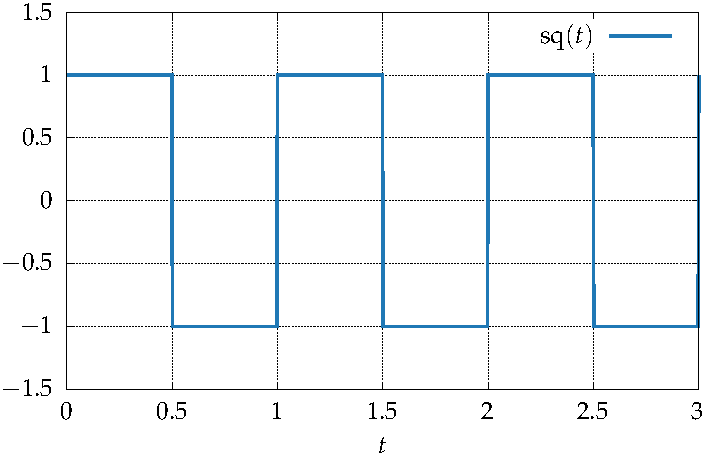
\includegraphics{gp_sq-wave.pdf}
  \caption{Curve of the square wave defined in~\cref{def:sq-wave}, the dots represent the
  values of the function at discontinuity points.}
  \label{fig:sq-wave}
\end{figure}

As anticipated in the previous chapter, fundamental building blocks for periodic functions
are the sine and cosine functions, which is the essence of Fourier analysis. It is
therefore useful to familiarise ourselves beforehand with periodic functions built using
sine and cosine, which is the topic of the next section.
%%%%%%%%%%%%%%%%%%%%%%%%%%%%%%%%%%%%%%%%%%%%%%%%%%%%%%%%%%%%%%%%%%%%%%%%%%%%%%%%%%%%%%%%%%
\section{Elementary waves}
We start by defining elementary sine waves
\begin{definition}
  \label{def:sine-wave}
  We call \emph{elementary sine wave} the function defined by
  \begin{equation}
    \sw(t;\omega,\phi)=\sin(2\pi\omega t + \phi)\,.\label{eq:sine-wave}
  \end{equation}
  where $\omega\neq 0$ and $0\leq\phi<2\pi$ are the \emph{frequency} and \emph{phase} of
  the wave, respectively. When the phase argument is omitted then it is assumed that
  $\phi=0$, \ie $\sw(t;\omega)=\sw(t;\omega,0)$. If the variable $t$ is omitted, the
  notation $\sw(\omega,\phi)$ or $\sw(\omega)$ represents the function itself, \ie
  $\sw(\omega,\phi)(t)=\sw(t;\omega,\phi)$.
\end{definition}
\noindent It is straightforward to show that, according to the definition in the previous
section, $\sw(\omega,\phi)$ is a periodic function with fundamental frequency $|\omega|$
and amplitude $1$. The phase measures the delay in the oscillation relatively to a wave
with identical frequency equal to zero at $t=0$. More generally if two waves have
identical frequencies and different phases $\phi_1$ and $\phi_2$, the time delay between
them is given by
\begin{equation}
  \delta t =\frac{\tau}{2\pi}\delta\phi\qquad\text{with}\qquad\delta\phi=\phi_1-\phi_2\,,
\end{equation}
with the fundamental period $\tau=\frac{1}{\omega}$. More explicitly,
\begin{equation}
  \sw(t;\omega,\phi_1)=\sw(t+\delta t;\omega,\phi_2)\,.
\end{equation}
In other words, the phase can always be re-written as a shift in time:
\begin{equation}
  \sw(t;\omega,\phi)=\sw(t+t_0;\omega),
  \qquad\text{with}\qquad
  t_0 = \frac{\tau\phi}{2\pi}\,.\label{eq:phase-delay}
\end{equation}
The frequency and phase are represented graphically in~\cref{fig:sine-wave}.
\begin{figure}[t]
  \centering
  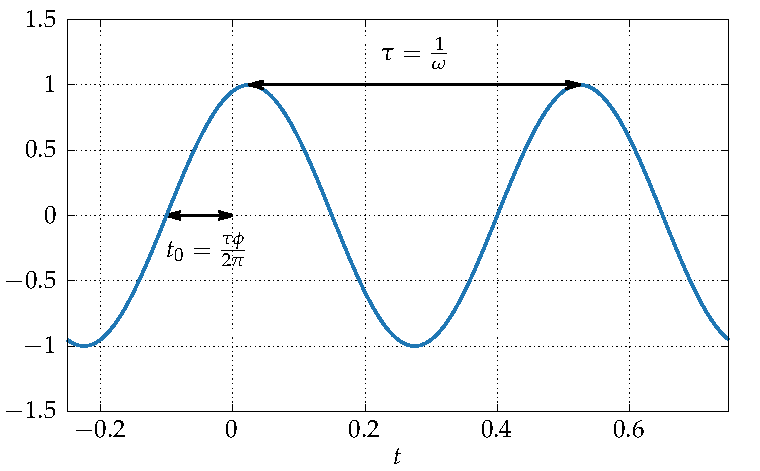
\includegraphics{gp_sine-wave.pdf}
  \caption{Example curve of the sine wave defined in~\cref{eq:sine-wave}, with frequency
    $\omega=2$ and phase $\phi=0.2\times 2\pi$. The arrows represent the period $\tau$ and
  the phase delay from~\cref{eq:phase-delay}.}
  \label{fig:sine-wave}
\end{figure}
For the special phase $\frac{\pi}{2}$, a sine wave can be written using the cosine
function:
\begin{equation}
  \sw\left(t;\omega,\frac{\pi}{2}\right)= \cos(2\pi\omega t)\,,
\end{equation}
motivating the following definition
\begin{definition}
  \label{def:cosine-wave}
  We call \emph{elementary cosine wave} the function
  \begin{equation}
    \cw(t;\omega,\phi)=\cos(2\pi\omega t + \phi)\,.\label{eq:cosine-wave}
  \end{equation}
  Similarly to the case of sine waves we define $\cw(t;\omega)=\cw(t;\omega,0)$, and
  $\cw(\omega,\phi)$ or $\cw(\omega)$ represents the function itself. Sine and cosine
  waves are related by the following phase relationships
  \begin{equation}
    \sw(t;\omega,\phi)=\cw\left(t;\omega,\phi-\frac{\pi}{2}\right),
    \quad\text{and}\quad
    \cw(t;\omega,\phi)=\sw\left(t;\omega,\phi+\frac{\pi}{2}\right)\,.
  \end{equation}
\end{definition}
A crucial set of formula to manipulate waves is given by the angle addition theorem:
\begin{theorem}[Angle addition]
  \label{thm:angle-add}
  For all pairs of real numbers $a$ and $b$, the following identities hold
  \begin{align}
    \sin(a+b)&=\sin(a)\cos(b)+\cos(a)\sin(b)\,,\label{eq:sinapb}\\
    \sin(a-b)&=\sin(a)\cos(b)-\cos(a)\sin(b)\,,\label{eq:sinamb}\\
    \cos(a+b)&=\cos(a)\cos(b)-\sin(a)\sin(b)\,,\label{eq:cosapb}\\
    \cos(a-b)&=\cos(a)\cos(b)+\sin(a)\sin(b)\,.\label{eq:cosamb}
  \end{align}
\end{theorem}
\begin{proof}
  We remind that the sine and cosine function are the real and imaginary part of the
  exponential of a purely imaginary number, namely for all $\theta\in\mathbb{R}$,
  \begin{equation}
    e^{i\theta}=\cos(\theta)+i\sin(\theta)\,.
  \end{equation}
  Therefore,
  \begin{equation}
    e^{i a}e^{i b}=\cos(a)\cos(b)-\sin(a)\sin(b)+i[\cos(a)\sin(b)+\sin(a)\cos(b)]\,,
    \label{eq:eaeb}
  \end{equation}
  and by definition
  \begin{equation}
    e^{i(a+b)}=\cos(a+b)+i\sin(a+b)\,.\label{eq:eapb}
  \end{equation}
  Now, using the fact that $e^{i(a+b)}=e^{i a}e^{i b}$, and identifying the real and
  imaginary parts in~\cref{eq:eaeb,eq:eapb}, one directly
  obtains~\cref{eq:sinapb,eq:cosapb}. \cref{eq:sinamb,eq:cosamb} can then be obtained
  using the parity properties of the sine and cosine functions, namely $\sin(-x)=-\sin(x)$
  and $\cos(-x)=\cos(x)$.
\end{proof}
This theorem can be used to produce additional identities for the sums and products of
sine and cosine functions:
\begin{corollary}
  \label{cor:sumproduct}
  For all pairs of real numbers $a$ and $b$, the following identities hold
  \begin{align}
    \sin(a)\sin(b)&=\frac{1}{2}\left[\cos(a-b)-\cos(a+b)\right]\,,
    \label{eq:sinatsinb}\\
    \sin(a)\cos(b)&=\frac{1}{2}\left[\sin(a-b)+\sin(a+b)\right]\,,
    \label{eq:sinatcosb}\\
    \cos(a)\cos(b)&=\frac{1}{2}\left[\cos(a-b)+\cos(a+b)\right]\,,
    \label{eq:cosatcosb}\\
    \sin(a)+\sin(b)&=2\sin\left(\frac{a+b}{2}\right)\cos\left(\frac{a-b}{2}\right)\,,
    \label{eq:sinapsinb}\\
    \cos(a)+\cos(b)&=2\cos\left(\frac{a+b}{2}\right)\cos\left(\frac{a-b}{2}\right)\,.
    \label{eq:cosapcosb}
  \end{align}
\end{corollary}
\begin{proof}
  \cref{eq:sinatsinb,eq:cosatcosb} are obtained by considering the sum and difference
  of~\cref{eq:cosapb,eq:cosamb}, and~\cref{eq:sinatcosb} by taking the sum
  of~\cref{eq:sinapb,eq:sinamb}. Then, we define
  \begin{equation}
    c=\frac{a+b}{2}\qquad\text{and}\qquad d=\frac{a-b}{2}\,,
  \end{equation}
  which implies that $a=c+d$ and $b=c-d$. Now, using~\cref{eq:sinatcosb} leads to
  \begin{align}
    \sin(a)+\sin(b)&=\sin(c+d)+\sin(c-d)=2\sin(c)\cos(d)\notag\\
    &=2\sin\left(\frac{a+b}{2}\right)\cos\left(\frac{a-b}{2}\right)\,,
  \end{align}
  which proves~\cref{eq:sinapsinb}. \cref{eq:cosapcosb} can be derived in the same way
  using~\cref{eq:cosatcosb}.
\end{proof}
These additional formulas allow to systematically convert a product of sine/cosine
functions into a sum, and vice-versa. The angle addition theorem can be proven solely
using triangle geometry, which is significantly less trivial than the simple proof above,
based on complex numbers. Elementary waves can generally be easier to manipulate using
complex exponentials, motivating the definition below.
\begin{definition}
  \label{def:complex-wave}
  We call \emph{elementary complex wave} the function
  \begin{equation}
    \ew(t;\omega,\phi)=e^{i(2\pi\omega t + \phi)}\,.
  \end{equation}
  As previously we define $\ew(t;\omega)=\ew(t;\omega,0)$, and $\ew(\omega,\phi)$ or
  $\ew(\omega)$ represents the function itself. By definition of the complex exponential,
  elementary complex waves are related to sine and cosine elementary waves by the relation
  \begin{equation}
    \ew(t;\omega,\phi)=\cw(t;\omega,\phi)+i\sw(t;\omega,\phi)\,,
  \end{equation}
  Thanks to the properties of the exponential, we have the two following trivial
  relationships
  \begin{equation}
    \ew(t;\omega,\phi)=e^{i\phi}\ew(t;\omega)\,\quad\text{and}\quad
    \ew(t;\omega,\phi)^*=\ew(-t;\omega,-\phi)=\ew(t;-\omega,-\phi)\,,\label{eq:cw-conj}
  \end{equation}
  Using these formulas, the relationship to sine and cosine waves can be rewritten as
  \begin{align}
    \cw(t;\omega,\phi)&=\frac{1}{2}[\ew(t;\omega,\phi)+\ew(t;-\omega,-\phi)]\,,
    \label{eq:cwtoew}\\
    \sw(t;\omega,\phi)&=-\frac{i}{2}[\ew(t;\omega,\phi)-\ew(t;-\omega,-\phi)]\,.
    \label{eq:swtoew}
  \end{align}
\end{definition}
A considerable simplification with complex waves comes from the fact that the phase just
leads to a multiplicative factor, equivalent to giving a \emph{complex amplitude} to the
wave. Similarly, phased sine and cosine waves can be expressed as a sum of zero-phase ones
using the angle addition theorem:
\begin{align}
  \sw(t;\omega,\phi)&=\cos(\phi)\sw(t;\omega)+\sin(\phi)\cw(t;\omega)\,,\\
  \cw(t;\omega,\phi)&=\cos(\phi)\cw(t;\omega)-\sin(\phi)\sw(t;\omega)\,.
\end{align}
%%%%%%%%%%%%%%%%%%%%%%%%%%%%%%%%%%%%%%%%%%%%%%%%%%%%%%%%%%%%%%%%%%%%%%%%%%%%%%%%%%%%%%%%%%
\section{Combination of elementary waves}
We will now discuss how to create more general waves by adding elementary waves. One first
legitimate question is whether the sum of two periodic functions is till periodic. It is
not always true, and can be a non-trivial topic, characterised in part by the following
result:
\begin{theorem}
  \label{thm:period-sum}
  Let $f_1(t)$ and $f_2(t)$ be two periodic functions of fundamental periods $\tau_1\neq
  0$ and $\tau_2\neq 0$, respectively. Then if the period ratio
  $\smash{\frac{\tau_1}{\tau_2}}$ is a rational number, then the sum $f_1+f_2$, as well as
  the product $f_1f_2$, are periodic. If $f_1$ and $f_2$ are continuous, the rationality
  of $\smash{\frac{\tau_1}{\tau_2}}$ becomes a necessary condition.
\end{theorem}
\begin{proof}
  We start by assuming that $\frac{\tau_1}{\tau_2}$ is a rational number. Then there
  exists two non-zero integers $p$ and $q$ such that $\frac{\tau_1}{\tau_2}=\frac{p}{q}$,
  and therefore
  \begin{equation}
    q\tau_1=p\tau_2\,.
  \end{equation}
  Then
  \begin{equation}
    f_1(t+q\tau_1)f_2(t+q\tau_1)=f_1(t+q\tau_1)f_2(t+p\tau_2)=f_1(t)f_2(t)\,,
  \end{equation}
  so $q\tau_1=p\tau_2$ is a period of $f_1f_2$. The same argument applies identically to
  the sum $f_1+f_2$. We will admit here the non-trivial fact that if $f_1+f_2$ is
  continuous and $f_1$ and $f_2$ are continuous, $\frac{\tau_1}{\tau_2}$ is necessarily a
  rational number.
\end{proof}
\begin{example}
  \label{ex:period-sum}
  $\sin\left(\frac{2\pi}{3}t\right)+\sin(\pi t)$ is periodic with fundamental period $6$.
\end{example}
\begin{example}
  \label{ex:nperiod-sum}
  $\sin(t)+\sin(\pi t)$ is not periodic.
\end{example}
\noindent Both examples above are illustrated in~\cref{fig:sine-sum}. Mathematically
speaking,~\cref{thm:period-sum} means that generally periodic functions sums are not
periodic. However, we remind the reader that any real number is arbitrarily close to a
rational number, so non-periodic sums like in~\cref{ex:nperiod-sum} can always be
approximated arbitrarily well by a periodic function. This is relevant for physics and
engineering applications where quantities are often known up to some limited precision.
\begin{figure}[t]
  \centering
  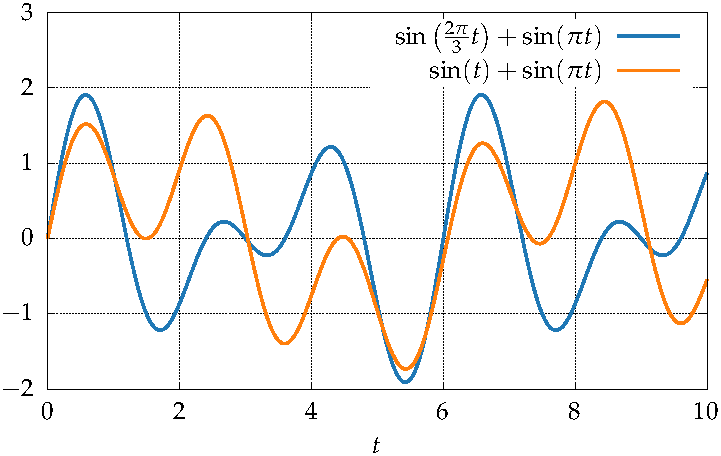
\includegraphics{gp_sine-sum.pdf}
  \caption{Curves of the sine wave sums in~\cref{ex:period-sum,ex:nperiod-sum}}
  \label{fig:sine-sum}
\end{figure}

Regarding elementary waves, one can demonstrate easily using the angle addition theorem
that products can always be reduced to sums:
\begin{proposition}
  The following identities hold for multiplying elementary waves:
  \begin{align}
    \cw(\omega_1)\cw(\omega_2)&=\frac{1}{2}[\cw(\omega_1-\omega_2)+\cw(\omega_1+\omega_2)]
    \label{eq:cprod}\\
    \sw(\omega_1)\sw(\omega_2)&=\frac{1}{2}[\cw(\omega_1-\omega_2)-\cw(\omega_1+\omega_2)]
    \label{eq:sprod}\\
    \sw(\omega_1)\cw(\omega_2)&=\frac{1}{2}[\sw(\omega_1-\omega_2)+\sw(\omega_1+\omega_2)]
    \label{eq:scprod}\\
    \ew(\omega_1)\ew(\omega_2)&=\ew(\omega_1+\omega_2)\label{eq:eprod}
  \end{align}
\end{proposition}
\begin{proof}
  These identities are a trivial re-interpretation of~\cref{cor:sumproduct}.
\end{proof}

An important concept when adding waves is the notion of \emph{interference}. Waves
oscillate between negative and positive values (or around the unit circle for complex
waves), and can add up or cancel when summed. This can be formalised in the following way
\begin{definition}
  Let $f$ and $g$ be two complex-valued periodic functions, not necessarily with the same
  period. We consider the sum $h=f+g$, which modulus squared is given by
  \begin{equation}
    |h|^2=|f|^2+|g|^2+2\Re(f^*g)\,.
  \end{equation}
  The last term $2\Re(f^*g)$ in the equation is called the \emph{interference term}. At a
  given point $t\in\mathbb{R}$:
  \begin{enumerate}
    \item if $\Re[f^*(t)g(t)]>0$, $f$ and $g$ are said to \emph{interfere constructively}
      at $t$;
    \item if $\Re[f^*(t)g(t)]<0$, $f$ and $g$ are said to \emph{interfere destructively}
      at $t$.
  \end{enumerate}
  If $f$ and $g$ are real-valued functions, the interference term is simply given by
  $2fg$.
\end{definition}
We now discuss below key examples of interference between elementary waves.
\begin{example}
  We consider the sum of two sine waves with equal frequencies, but different phases:
  \begin{equation}
    f(t)=\sw(t;\omega)+\sw(t;\omega,\phi)\,.
  \end{equation}
  Using~\cref{eq:sinapsinb}, $f(t)$ can be re-written as
  \begin{equation}
    f(t)=2\cos\left(\frac{\phi}{2}\right)\sw\left(t;\omega,\frac{\phi}{2}\right)\,.
  \end{equation}
  So $f$ is still an elementary sine wave with frequency $\omega$, phase $\frac{\phi}{2}$,
  and amplitude $2\cos(\frac{\phi}{2})$. The interesting element here is the change of
  amplitude: at $\phi=0$, the amplitude of $f$ is $2$, and the two waves interfere in a
  maximally constructive way, they are said to be \emph{in phase}. At $\phi=\pi$, $f$ is
  identically zero and the two waves interfere in a maximally destructive way, they are
  said to be \emph{out of phase}. Using the definition above, and~\cref{eq:sinatsinb}, the
  related interference term is given by
  \begin{equation}
    2\sw(t;\omega,\phi)\sw(t;\omega)=\cos(\phi)-\cw(t;2\omega,\phi)\,.
  \end{equation}
  Because the cosine function oscillate between $-1$ and $1$, the expression above takes
  values between $-2$ and $2$. If $\phi=0$, the two waves interfere constructively for all
  $t$, which is the maximally constructive case above. Similarly, the waves interfere
  destructively for all $t$ with $\phi=\pi$. This example is illustrated
  in~\cref{fig:interference}
\end{example}
\begin{figure}[ph!]
  \centering
  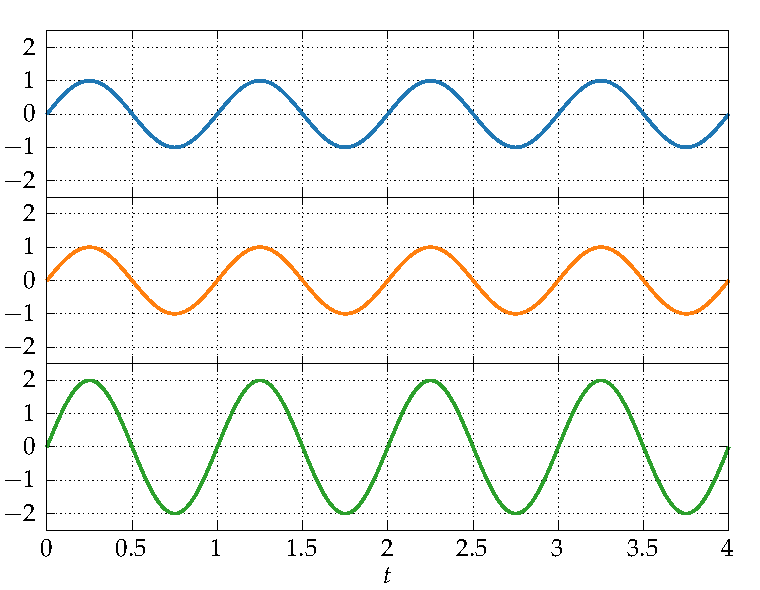
\includegraphics{gp_sine-interference.pdf}
  \\\hspace{0.2cm}(a)\\~\\
  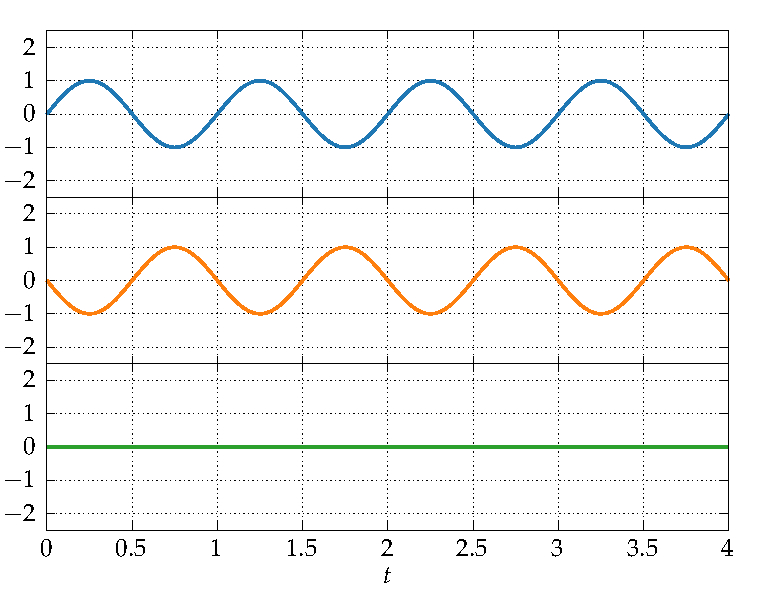
\includegraphics{gp_sine-interference-des.pdf}
  \\\hspace{0.2cm}(b)\\
  \caption{For each figure above, the lowermost curve represent the sum of the two curves
    above. Pane (a) represents a case of maximally constructive interference between two
    in-phase sine waves with frequency $1$. Pane (b) represents a case of maximally
  destructive interference between two out-of-phase sine waves with frequency $1$.}
  \label{fig:interference}
\end{figure}
\begin{example}
  Another important example of interference is the \emph{beating effect}, which occurs
  when summing two elementary waves with slightly different frequencies:
  \begin{equation}
    f(t)=\sw(t;\omega)+\sw(t;\omega+\delta\omega)\,,
  \end{equation}
  where $\delta\omega$ is assumed to be small compared to $\omega$. In this case, the
  interference term can be written
  \begin{equation}
    2\sw(t;\omega)\sw(t;\omega+\delta\omega)=\cw(t;\delta\omega)-\cw(t;2\omega+\delta\omega)
    \simeq \cw(t;\delta\omega)-\cw(t;2\omega)\,,
  \end{equation}
  where in the last term we used the assumption on the smallness of $\delta\omega$. The
  first cosine in this expression oscillates much slower than the second one, and is equal
  to $1$ for $t=\smash{\frac{n}{\delta\omega}}$, and $-1$ for
  $t=\smash{\frac{n}{\delta\omega}+\frac{1}{2\delta\omega}}$. Following the same argument
  as in the previous example, this means that $f(t)$ oscillates in time between maximally
  constructive and destructive interference, at the frequency $\delta\omega$. This is
  generally called a \emph{beating effect}, particularly in an acoustic context, where the
  intensity of the sound associated to $f(t)$ very distinctly goes to zero periodically
  $\delta\omega$ times per second.

  Another way to present this phenomenon is to write the identity
  \begin{equation}
    f(t)=2\cw\left(t;\frac{\delta\omega}{2}\right)
    \sw\left(t;\omega+\frac{\delta\omega}{2}\right)
    \simeq 2\cw\left(t;\frac{\delta\omega}{2}\right)\sw(t;\omega)\,.
  \end{equation}
  In that form, $f(t)$ appears as a sine wave with frequency $\omega$ modulated by a
  cosine with half this frequency. Since the cosine function goes to zero twice per
  period, we find again that $f(t)$ goes to zero with frequency $\delta\omega$. The
  beating effect is illustrated in~\cref{fig:beating}.
\end{example}
\begin{figure}
  \centering
  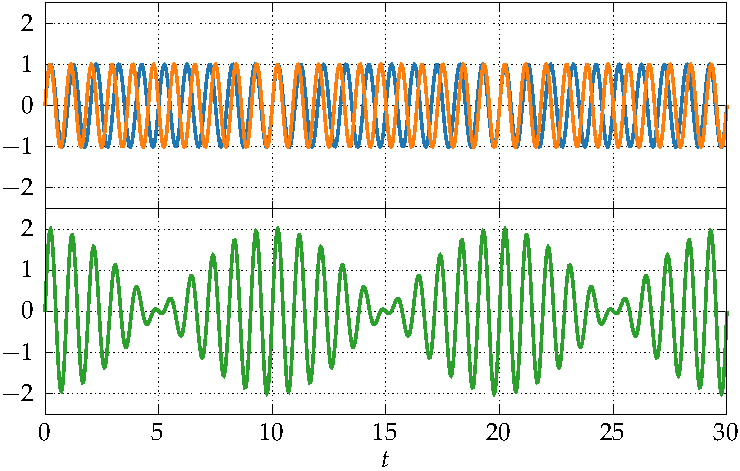
\includegraphics{gp_sine-beating.pdf}
  \caption{The upper plot represents two sine waves with slightly different frequencies
    $\omega=1$ and $\omega+\delta\omega=1.1$. The lower plot represents the sum of these
    two waves, with a visible beating effect with frequency $\delta\omega=0.1$. The beats
  can be correlated with the two sine waves going in and out of phase.}
  \label{fig:beating}
\end{figure}
%%%%%%%%%%%%%%%%%%%%%%%%%%%%%%%%%%%%%%%%%%%%%%%%%%%%%%%%%%%%%%%%%%%%%%%%%%%%%%%%%%%%%%%%%%
\section{Trigonometric polynomials}
We can make the following definition for an arbitrary linear combination of elementary
waves:
\begin{definition}
  We call \emph{trigonometric polynomial} of degree $N$ and frequency $\omega$ any
  function of the form
  \begin{equation}
    P(t)=\frac{a_0}{2}+\sum_{n=1}^N[a_n\cw(t;n\omega)+b_n\sw(t;n\omega)]\,,
    \label{eq:trigp-sc}
  \end{equation}
  where $a_n$ and $b_n$ are real coefficients such that $a_N\neq 0$ or $b_N \neq 0$. The
  formula above is called the \emph{sine-cosine form} of $P(t)$ with \emph{sine-cosine
  coefficients} or \emph{modes} $a_n$ and $b_n$. The $\frac{1}{2}$ normalisation of $a_0$
  is arbitrary, and will be convenient later. It is also convenient to define $b_0=0$, to
  avoid constantly treating the $a_n$ coefficients separately for having an $n=0$
  coefficient.
\end{definition}
It is clear that such function is periodic, and a consequence of~\cref{thm:period-sum} is
then
\begin{proposition}
  Let $P$ be a trigonometric polynomial of degree $N\geq 1$ and frequency $\omega$ with
  sine-cosine coefficients $a_n$ and $b_n$. $P$ is a periodic function with period
  $\tau=\frac{1}{\omega}$, and additionally if $a_1\neq0$ or $b_1\neq0$, then $\omega$ is
  the fundamental frequency of $P(t)$.
\end{proposition}
\begin{proof}
  Each term in~\cref{eq:trigp-sc} is trivially $T$-periodic, so $P$ is also
  $\tau$-periodic. Now, the $n$-th mode of $P$ has a fundamental period of
  $\tau_n=\frac{\tau}{n}$. Assuming that $a_1\neq0$ or $b_1\neq0$, then the period ratio
  of this first mode to an arbitrary non-vanishing higher mode $n$ is given by
  \begin{equation}
    \frac{\tau_1}{\tau_n}=n\,.
  \end{equation}
  Using~\cref{thm:period-sum}, this means that this combination of modes has fundamental
  period $\tau$. The remaining modes can then be added one after another, and repeated use
  of~\cref{thm:period-sum} demonstrate the proposition.
\end{proof}
As we previously did for the elementary waves, trigonometric polynomials can be put in a
convenient complex form
\begin{definition}
  \label{def:trigp-complex}
  Let $P$ be a trigonometric polynomial of degree $N$ and frequency $\omega$ with
  sine-cosine coefficients $a_n$ and $b_n$. $P$ can be written in the \emph{complex form}
  \begin{equation}
    P(t)=\sum_{n=-N}^{N}c_n\ew(t;n\omega)\,,\label{eq:trigp-complex}
  \end{equation}
  with the \emph{complex coefficients}
  \begin{equation}
    c_n =
    \begin{cases}
      \frac{1}{2}(a_n-ib_n)&\text{if~}n< 0\\
      \frac{1}{2}(a_n+ib_n)&\text{if~}n\geq 0
    \end{cases}
    \,,\label{eq:ab-to-c}
  \end{equation}
  which have the property $c_n^*=c_{-n}$. The relation above can be inverted to
  \begin{equation}
    a_n=c_n+c_{-n}\qquad\text{and}\qquad
    b_n=i(c_n-c_{-n})\,.
  \end{equation}
\end{definition}
The formulas in the definition above can be obtained using~\cref{eq:cwtoew,eq:swtoew} with
the definition~\cref{eq:trigp-sc}, which is left as an exercise to the reader. A key
property of trigonometric polynomials, that will be crucial later, is the unicity of their
coefficients, formulated in the theorem below
\begin{theorem}
  \label{thm:trigp-unicity}
  Let $P$ and $Q$ be two trigonometric polynomials with the same frequency $\omega$,
  degrees $N$ and $N'$, and sine-cosine coefficients $a_n$,$b_n$ and $a'_n$,$b'_n$,
  respectively. $P$ and $Q$ are identically equal,~\ie $P(t)=Q(t)$ for all
  $t\in\mathbb{R}$, if and only if their degrees and coefficients are equal, \ie $N=N'$
  and for all $n$
  \begin{equation}
    a_n=a'_n\quad\text{and}\quad b_n=b'_n\,.
  \end{equation}
\end{theorem}
Although we could attempt to prove that directly, this theorem is a consequence of
fundamental orthogonality properties of elementary waves. Because these properties are
crucial in Fourier analysis, we  study them in detail in the next section, where the
theorem above will be proven.

%%%%%%%%%%%%%%%%%%%%%%%%%%%%%%%%%%%%%%%%%%%%%%%%%%%%%%%%%%%%%%%%%%%%%%%%%%%%%%%%%%%%%%%%%%
\section{Orthogonality of elementary waves}
The reader might be more familiar with the notion of orthogonality in vector spaces, which
we summarise below as an introduction to the notion of orthogonality of periodic
functions. In vector calculus, given an $n$-dimensional real vector $\vec{v}$ and a unit
vector $\vec{u}$, the \emph{orthogonal projection} $\vec{v}_{\vec{u}}$ of $\vec{v}$ on the
axis defined by $\vec{u}$ is given by
\begin{equation}
  \label{eq:orth-proj}
  \vec{v}_{\vec{u}}=\cos(\theta)|\vec{v}|\,\vec{u}\,,
\end{equation}
where $\theta$ is the angle between $\vec{u}$ and $\vec{v}$, and $|\vec{v}|$ is the norm
of $\vec{v}$. The projection coefficient $\cos(\theta)|\vec{v}|$ is known to be given by
the
\emph{dot product}
\begin{equation}
  \vec{v}\cdot \vec{u}=\sum_{j=1}^n \vec{v}_j \vec{u}_j=\cos(\theta)|\vec{v}|\,.
  \label{eq:vec-dot}
\end{equation}
Additionally, the dot product $\vec{v}\cdot \vec{u}$ vanishes when $\vec{v}$ and $\vec{u}$
are \emph{orthogonal} (\ie they form an angle of $\pi$ radians). This makes the dot
product an essential tool of vector calculus to compute the coordinate of vectors in an
orthonormal basis. Explicitly, let $\vec{e}_j$ be an orthonormal basis of $\mathbb{R}^n$,
and let $v^{\vec{e}}_j$ be the coefficients of $\vec{v}$ in that basis, \ie
\begin{equation}
  \vec{v}=\sum_{j=1}^{n}v^{\vec{e}}_j\,\vec{e}_j\,,
\end{equation}
then the $v^{\vec{e}}_j$ can be computed using the dot product using
\begin{equation}
  v^{\vec{e}}_j=\vec{v}\cdot \vec{e}_j\,.\label{eq:basis-proj}
\end{equation}
The concept of orthogonality and orthogonal projection can be generalised to more complex
mathematical objects like functions. As we discuss below, elementary waves can be
interpreted as an orthogonal basis for trigonometric polynomial, which is the reason
why~\cref{thm:trigp-unicity} holds, and a key structure at the heart of Fourier analysis.
Although the general description of orthogonality between functions is out of the scope of
this course and will not be treated here, this introduction to Fourier analysis can be
seen as a good introduction to this type of concept.
\begin{figure}[t]
  \caption{Visual representation of the orthogonal projection of a vector on a unit vector
  given in~\cref{eq:orth-proj}}
  \label{fig:orth-proj}
\end{figure}

We start by defining the dot product between two periodic functions
\begin{definition}
  \label{def:func-dot}
  Let $f$ and $g$ two real $\tau$-periodic functions. We assume that $f$ and $g$ are
  integrable on the interval $[0,\tau]$. The \emph{dot product} $\braket{f,g}$ between $f$
  and $g$ is the real number defined by
  \begin{equation}
    \braket{f,g}=\int_{0}^{\tau}\diff t\, f(t)g(t)\,.\label{eq:func-dot}
  \end{equation}
  Additionally, the \emph{$2$-norm} $\|f\|$ of the function $f$ is defined by
  \begin{equation}
    \|f\|^2=\braket{f,f}=\int_{0}^{\tau}\diff t\, f(t)^2\,.
  \end{equation}
\end{definition}
The definition~\cref{eq:func-dot} can be interpreted as a continuous version
of~\cref{eq:vec-dot}, where the values $f(t)$ and $g(t)$ are the ``continuous
coordinates'' of the functions $f$ and $g$, and the integral is a ``continuous sum'' over
these coordinates. The functional dot product has the same linearity and commutativity
properties than the vector dot product:
\begin{proposition}
  Let $f$, $g$, and $h$ be three real $\tau$-periodic functions. The following identities
  hold for any pair of real number $\alpha$ and $\beta$
  \begin{align}
    \braket{\alpha f+\beta g,h}&=\alpha\braket{f,h}+\beta\braket{g,h}\,,\\
    \braket{f,\alpha g+\beta h}&=\alpha\braket{f,g}+\beta\braket{f,h}\,,\\
    \braket{f,g}&=\braket{g,f}\,.
  \end{align}
\end{proposition}
\begin{proof}
  This is a trivial consequence of the definition~\cref{eq:func-dot} and the linearity of
  the integral.
\end{proof}
The definition of orthogonality follows naturally:
\begin{definition}
  \label{def:dot-rfunc}
  Let $f$ and $g$ be two $\tau$-periodic functions. $f$ and $g$ are said to be
  \emph{orthogonal} if their dot product vanishes, \ie
  \begin{equation}
    \braket{f,g}=0\,.
  \end{equation}
\end{definition}
We now give the main result of this section, \ie the orthogonality of elementary waves
\begin{theorem}
  \label{thm:sc-orth}
  Let $\omega>0$ be an arbitrary frequency corresponding to the period $\tau$. For any
  pair of integers $n$ and $m$, the following identities hold
  \begin{align}
    \braket{\sw(n\omega),\sw(m\omega)}&=\frac{\tau}{2}\delta_{nm}\,,\label{eq:sw-orth}\\
    \braket{\cw(n\omega),\cw(m\omega)}&=\frac{\tau}{2}\delta_{nm}\,,\label{eq:cw-orth}\\
    \braket{\cw(n\omega),\sw(m\omega)}&=0\,.\label{eq:scw-orth}
  \end{align}
  Where $\delta_{nm}$ is the \emph{Kronecker symbol}
  \begin{equation}
    \delta_{nm}=
    \begin{cases}
      1&~\mathrm{if}~~n=m\\
      0&~\mathrm{else}
    \end{cases}\,.
  \end{equation}
  In other words, for any pair of integers $n$ and $m$, sine waves of the form
  $\sw(n\omega)$ and $\sw(m\omega)$ have norm squared $\frac{\tau}{2}$ and are orthogonal
  if and only if $n\neq m$, the same applies to cosine waves, and a sine and a cosine wave
  of the form $\sw(n\omega)$ and $\cw(m\omega)$ are always orthogonal.
\end{theorem}
\begin{proof}
  Let us demonstrate~\cref{eq:sw-orth,eq:cw-orth,eq:scw-orth} using the
  definition~\cref{eq:func-dot}. We start with~\cref{eq:sw-orth}
  \begin{equation}
    \braket{\sw(n\omega),\sw(m\omega)}=\int_{0}^{\tau}\diff t\,
    \sin(2\pi n\omega t)\sin(2\pi m\omega t)\,.
  \end{equation}
  Using~\cref{eq:sprod}, one has
  \begin{equation}
    \sw(n\omega)\sw(m\omega)=\frac{1}{2}\{\cw[(n-m)\omega]-\cw[(n+m)\omega]\}\,.
    \label{eq:sw-prod}
  \end{equation}
  If $n=m$, this product simplifies to
  \begin{equation}
    \sw(n\omega)\sw(m\omega)=\frac{1}{2}[1-\cw(2n\omega)]\,,
  \end{equation}
  which integrates to
  \begin{equation}
    \frac{1}{2}\int_{0}^{\tau}\diff t\,[1-\cos(4\pi n\omega t)]=\frac{\tau}{2}-
    \left[\frac{1}{8\pi n\omega}\sin(4\pi n\omega t)\right]_0^\tau
    =\frac{\tau}{2}\,.
  \end{equation}
  If $n\neq m$, \cref{eq:sw-prod} integrates to
  \begin{align}
    &\frac{1}{2}\int_{0}^{\tau}\diff t\,\{\cos[2\pi(n-m)\omega t]-\cos[2\pi(n+m)\omega t]\}
    \notag\\
    &\qquad\qquad=\left[\frac{1}{2\pi(n-m)\omega}\sin[2\pi(n-m)\omega t]
    -\frac{1}{2\pi(n+m)\omega}\sin[2\pi(n+m)\omega t]\right]_0^\tau\notag\\
    &\qquad\qquad=0
  \end{align}
  Both equations above demonstrate~\cref{eq:sw-orth}. We now turn to~\cref{eq:cw-orth}, we
  start by using the product identity~\cref{eq:cprod}
  \begin{equation}
    \cw(n\omega)\cw(m\omega)=\frac{1}{2}\{\cw[(n-m)\omega]+\cw[(n+m)\omega]\}\,,
  \end{equation}
  which is identical to~\cref{eq:sw-prod} up to a sign. Retracing the steps above, the
  result for sine waves was independent of this sign, which implies that~\cref{eq:cw-orth}
  holds. Finally, using~\cref{eq:scprod}, we can write
  \begin{equation}
    \sw(n\omega)\cw(m\omega)=\frac{1}{2}\{\sw[(n-m)\omega]+\sw[(n+m)\omega]\}\,,
  \end{equation}
  which, if $n=m$, integrates to
  \begin{equation}
    \frac{1}{2}\int_{0}^{\tau}\diff t\,\sin(4\pi n\omega t)=
    \left[-\frac{1}{8\pi n\omega}\cos(4\pi n\omega t)\right]_0^T=0\,.
  \end{equation}
  In the case $n\neq m$, one obtains
  \begin{align}
    &\frac{1}{2}\int_{0}^{\tau}\diff t\,\{\sin[2\pi(n-m)\omega t]+\sin[2\pi(n+m)\omega t]\}
    \notag\\
    &\qquad\qquad=-\left[\frac{1}{2\pi(n-m)\omega}\cos[2\pi(n-m)\omega t]
    +\frac{1}{2\pi(n+m)\omega}\cos[2\pi(n+m)\omega t]\right]_0^\tau\notag\\
    &\qquad\qquad=0\,,
  \end{align}
  which demonstrates~\cref{eq:scw-orth}.
\end{proof}
One can also wonder about orthogonality properties of complex elementary waves. One issue
here is that the dot product from~\cref{def:dot-rfunc} was specifically defined for real
functions. It can be generalised to complex functions as follows
\begin{definition}
  Let $f$ and $g$ two complex $\tau$-periodic functions. We assume that $f$ and $g$ are
  integrable on the interval $[0,\tau]$. The \emph{dot product} $\braket{f,g}$ between $f$
  and $g$ is the complex number defined by
  \begin{equation}
    \braket{f,g}=\int_{0}^{\tau}\diff t\, f(t)g(t)^*\,.\label{eq:cfunc-dot}
  \end{equation}
  Additionally, the \emph{norm} $\|f\|$ of the function $f$ is the real number defined by
  \begin{equation}
    \|f\|^2=\braket{f,f}=\int_{0}^{\tau}\diff t\, |f(t)|^2\,.
  \end{equation}
\end{definition}
The generalisation is done by using a complex conjugation for the second argument of the
product, allowing the norm to remain a real positive number. Since any real number is its
own complex conjugate, this definition is clearly identical to~\cref{def:dot-rfunc} when
restricted to real functions. This generalisation has the consequence of slightly breaking
the symmetry of the dot product:
\begin{proposition}
  Let $f$, $g$, and $h$ be three complex $\tau$-periodic functions. The following
  identities hold for any pair of complex numbers $\alpha$ and $\beta$
  \begin{align}
    \braket{\alpha f+\beta g,h}&=\alpha\braket{f,h}+\beta\braket{g,h}\,,\\
    \braket{f,\alpha g+\beta h}&=\alpha^*\braket{f,g}+\beta^*\braket{f,h}\,,\\
    \braket{f,g}&=\braket{g,f}^*\,.
  \end{align}
\end{proposition}
\begin{proof}
  This is a trivial consequence of the definition~\cref{eq:cfunc-dot} and the linearity of
  the integral and complex conjugation.
\end{proof}
With this generalised dot product, we can formulate the orthogonality of complex
elementary waves
\begin{theorem}
  Let $\omega>0$ be an arbitrary frequency corresponding to the period $\tau$. For any
  pair of integers $n$ and $m$, the following identity holds
  \begin{equation}
    \braket{\ew(n\omega),\ew(m\omega)}=\tau\delta_{nm}\,,
  \end{equation}
  \ie for any pair of integers $n$ and $m$, complex elementary waves of the form
  $\ew(n\omega)$ and $\ew(m\omega)$ have norm squared $\tau$ and are orthogonal if and
  only if $n\neq m$.
\end{theorem}
\begin{proof}
  Using~\cref{eq:eprod,eq:cw-conj}, one has
  \begin{align}
    \braket{\ew(n\omega),\ew(m\omega)}&=\int_{0}^{\tau}\diff t\,\ew(t;n\omega)\ew(t;m\omega)^*
    =\int_{0}^{\tau}\diff t\,\ew(t;n\omega)\ew(t;-m\omega)\\
    &=\int_{0}^{\tau}\diff t\,e^{2\pi i (n-m)\omega t}\,.
  \end{align}
  If $n=m$, clearly
  \begin{equation}
    \braket{\ew(n\omega),\ew(m\omega)}=\tau\,,
  \end{equation}
  and if $n\neq m$
  \begin{equation}
    \braket{\ew(n\omega),\ew(m\omega)}=
    \left[\frac{1}{2\pi i (n-m)}e^{2\pi i (n-m)\omega t}\right]_0^\tau=0\,,
  \end{equation}
  which proves the theorem.
\end{proof}
One can notice, once again, that algebra is considerably simpler when using complex
elementary waves. We are now ready to prove~\cref{thm:trigp-unicity}:
\begin{proof}[Proof of~\cref{thm:trigp-unicity}]
  Let $P(t)$ and $P'(t)$ be two trigonometric polynomial of the general form
  \begin{align}
    P(t)&=a_0+\sum_{n=1}^N[a_n\,\cw(t;n\omega)+b_n\,\sw(t;n\omega)]\,,\\
    P'(t)&=a'_0+\sum_{n=1}^{N'}[a'_n\,\cw(t;n\omega)+b'_n\,\sw(t;n\omega)]\,.
  \end{align}
  We additionally assume that $P(t)$ and $P'(t)$ are identically equal, \ie
  \begin{equation}
    P(t)=P'(t)\,,
  \end{equation}
  for all real number $t$. This implies that for any integer $m$ one has
  \begin{equation}
    \braket{P,\cw(m\omega)}=\braket{P',\cw(m\omega)}\,.
  \end{equation}
  Using the orthogonality relations from~\cref{thm:sc-orth}, these dot products can be
  simplified to
  \begin{equation}
    \braket{P,\cw(m\omega)}=
    \begin{cases}
      \frac{\tau}{2}a_m&~\text{if}~m\leq N\\
      0&~\text{else}
    \end{cases},
    \quad\text{and}\quad
    \braket{P',\cw(m\omega)}=
    \begin{cases}
      \frac{\tau}{2}a'_m&~\text{if}~m\leq N'\\
      0&~\text{else}
    \end{cases}\,.
  \end{equation}
  Similarly,
  \begin{equation}
    \braket{P,\sw(m\omega)}=\braket{P',\sw(m\omega)}\,,
  \end{equation}
  and
  \begin{equation}
    \braket{P,\sw(m\omega)}=
    \begin{cases}
      \frac{\tau}{2}b_m&~\text{if}~m\leq N\\
      0&~\text{else}
    \end{cases},
    \quad\text{and}\quad
    \braket{P',\sw(m\omega)}=
    \begin{cases}
      \frac{\tau}{2}b'_m&~\text{if}~m\leq N'\\
      0&~\text{else}
    \end{cases}\,.
  \end{equation}
  Combining the equalities above implies directly that $a_n=a'_n$ and $b_n=b'_n$ for all
  $n$.
\end{proof}
We can notice that~\cref{thm:trigp-unicity} is somewhat trivial when one knows the
orthogonality relationships between sine and cosine waves. This also generalises a
well-known property from vector calculus: a set of orthogonal vectors defines a unique
coordinate system, and these coordinates can be obtained using orthogonal projection on
the basis vectors as in~\cref{eq:basis-proj}. Finally, \cref{thm:trigp-unicity}
generalises naturally to the complex form of trigonometric polynomials:
\begin{corollary}
  \label{corr:trigp-unicity-cplx}
  Let $P$ and $Q$ be two trigonometric polynomials with the same frequency $\omega$,
  degrees $N$ and $N'$, and complex coefficients $c_n$ and $c'_n$, respectively. $P$ and
  $Q$ are identically equal,~\ie $P(t)=Q(t)$ for all $t$, if and only if their degrees and
  coefficients are equal, \ie $N=N'$ and for all $n$
  \begin{equation}
    c_n=c'_n\,.
  \end{equation}
\end{corollary}
\begin{proof}
  Using~\cref{thm:trigp-unicity}, we know that the sine-cosine coefficients of the
  polynomials are unique. We also saw in~\cref{eq:ab-to-c} that complex coefficients are
  uniquely defined from the sine-cosine ones, which proves the coronary. Another way to
  prove this result is, similarly to the proof of~\cref{thm:trigp-unicity}, to project $P$
  in the form~\cref{eq:trigp-complex} on complex waves:
  \begin{equation}
    \braket{P,\ew(m\omega)}=
    \begin{cases}
      \tau c_m&~\text{if}~m\leq N\\
      0&~\text{else}
    \end{cases}\,,
  \end{equation}
  which, as previously, provides a unique determination of the $c_m$ coefficients given
  $P$.
\end{proof}
This concludes this section on the orthogonality of elementary waves. We will now discuss
how to generalise elementary waves and trigonometric polynomials to multiple real
variables.
%%%%%%%%%%%%%%%%%%%%%%%%%%%%%%%%%%%%%%%%%%%%%%%%%%%%%%%%%%%%%%%%%%%%%%%%%%%%%%%%%%%%%%%%%%
\section{Elementary waves in multiple dimensions}
In all this chapter, we discussed elementary waves and their combinations as functions of
a single real variable. However, oscillatory physical systems will often require multiple
variables to be described. We already encountered that in~\cref{chap:wave-eq} when
studying the wave equation. We found that the wave equation
solution~\cref{eq:string-fourier} for the plucked string was a periodic function both in
the time and space dimensions. Before starting to discuss how this result can help us to
define trigonometric polynomials in multiple dimensions, we need to formulate a definition
for multidimensional periodic functions. This can be done simply by considering functions
that are periodic in each of their variables:
\begin{definition}
  A function $f$ on $\mathbb{R}^d$ is said to be \emph{periodic} or specifically
  \emph{$\vec{\tau}$-periodic} if there exists a vector $\vec{\tau}$ with positive
  components such that $f(\vec{x})=f(x_1,\dots,x_d)$ is $\tau_j$-periodic in the variable
  $x_j$, for all directions $j$. The vector $\vec{\tau}$ is called a \emph{period} of $f$,
  and the vector $\vec{\omega}$ defined by
  \begin{equation}
    \omega_j=\frac{1}{\tau_j}\,,
  \end{equation}
  is called a \emph{frequency} of $f$.
\end{definition}
\begin{example}
  The function $f$ defined by $f(x,y)=\sin(x+2y)$ is $(2\pi,\pi)$-periodic.
\end{example}

\begin{figure}[t]
  \centering
  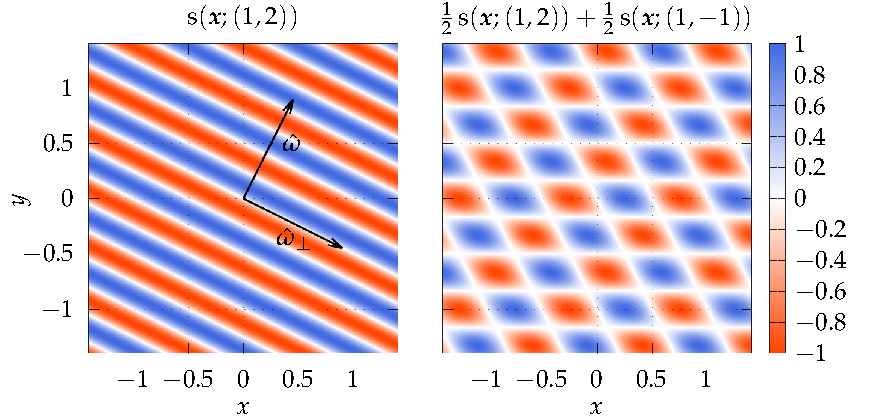
\includegraphics{gp_wave-plane.pdf}
  \caption{The left pane represents the plane wave $\sw(\vec{x};\vec{\omega})$, with
    $\vec{x}=(x,y)$ and $\vec{\omega}=(1,2)$. The arrows represent the unit vectors
    $\hat{\bm{\omega}}=(1,2)/\sqrt{5}$, and $\hat{\bm{\omega}}_{\perp}=(2,-1)/\sqrt{5}$ in
    the perpendicular direction. The right pane shows the interference pattern emerging
  when adding two plane sine waves with wave vectors $(1,2)$ and $(1,-1)$.}
  \label{fig:plane-wave}
\end{figure}
\begin{figure}[t]
  \centering
  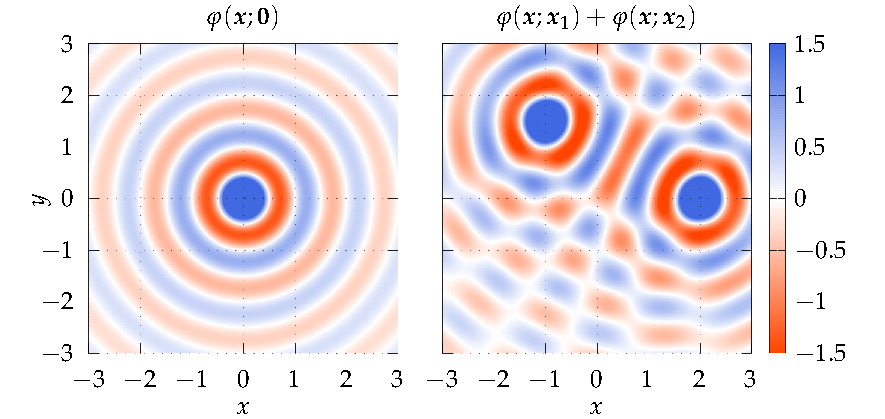
\includegraphics{gp_wave-sphere.pdf}
  \caption{The left pane represents the spherical wave $\varphi(\vec{x};\vec{0})$, with
    $\vec{x}=(x,y)$, defined in~\cref{eq:sphere-wave}. The right pane shows an example of
    interference patten between two spherical waves with source positions
    $\vec{x}_1=(-1,1.5)$ and $\vec{x}_2=(0,2)$. Although the maximum magnitude of
    $\varphi$ is $2\pi=6.28$, the colour scale was limited to the interval $[-1.5,1.5]$
  for visibility.}
  \label{fig:sphere-wave}
\end{figure}
We could inspire ourselves from the solution~\cref{eq:string-fourier} of the plucked
string problem to define trigonometric polynomials in $d$ dimensions to be linear
combinations of products of $d$ elementary sine or cosine waves. Although this would be a
fine definition, it would need a tedious discussion of the combinatorics of all the
possible independent cross-terms between sine and cosine waves. This is, once more, a
situation where using complex exponentials brings considerable simplifications, since the
product of complex waves is still a complex wave. Explicitly, assuming a vector of $d$
real variables $\vec{x}=(x_1,\dots,x_d)$, and a vector of $d$ frequencies
$\vec{\omega}=(\omega_1,\dots,\omega_d)$, we can write
\begin{align}
  e^{2\pi i\omega_1x_1}\cdots e^{2\pi i\omega_dx_d}
  &=e^{2\pi i(\omega_1x_1+\cdots+\omega_dx_d)}=e^{2\pi i\vec{\omega}\cdotp\vec{x}}\notag\\
  &=\cos(2\pi\vec{\omega}\cdot\vec{x})+i\sin(2\pi\vec{\omega}\cdot\vec{x})\,.
\end{align}
This motivates the following definitions for multidimensional elementary waves
\begin{definition}
  \label{def:multidim-waves}
  We call \emph{elementary sine wave}, \emph{elementary cosine wave}, and \emph{elementary
  complex wave} on $\mathbb{R}^d$ the functions defined by
  \begin{align}
    \sw(\vec{x};\vec{\omega},\phi)&=\sin(2\pi\vec{\omega}\cdot\vec{x}+\phi)\,,\\
    \cw(\vec{x};\vec{\omega},\phi)&=\cos(2\pi\vec{\omega}\cdot\vec{x}+\phi)\,,\\
    \ew(\vec{x};\vec{\omega},\phi)&=e^{2\pi i\vec{\omega}\cdotp\vec{x}+\phi}\,,
  \end{align}
  respectively, where the \emph{wave vector} $\vec{\omega}\in\mathbb{R}^d$ has only
  non-zero components, and the \emph{phase} $\phi$ is a real number such that $0\leq \phi
  <2\pi$.
\end{definition}
Because multidimensional elementary waves are essentially defined as one-dimensional waves
applied on a dot product, most identities from the previous section can be easily
generalised. The previous statement can be investigated further in the following way: for
a given wave vector $\vec{\omega}$, any vector $\vec{x}$ can be uniquely written as
\begin{equation}
  \vec{x}=\vec{x}_{\parallel}+\vec{x}_{\perp}\,,
\end{equation}
where $\vec{x}_{\parallel}$ is the orthogonal projection of $\vec{x}$ on $\vec{\omega}$,
and $\vec{x}_{\perp}$ is the perpendicular remainder. Explicitly
\begin{equation}
  \vec{x}_{\parallel}=(\vec{x}\cdot\hat{\vec{\omega}})\,\hat{\vec{\omega}}
  \qquad\text{and}\qquad
  \vec{x}_{\perp}=\vec{x}-\vec{x}_{\parallel}\,,
\end{equation}
where $\hat{\vec{\omega}}$ is the unit vector in the direction of $\vec{\omega}$, \ie
\begin{equation}
  \hat{\vec{\omega}}=\frac{\vec{\omega}}{|\vec{\omega}|}\,.
\end{equation}
One can check explicitly that $\vec{x}_{\perp}$ is indeed orthogonal to $\vec{\omega}$:
\begin{equation}
  \vec{x}_{\perp}\cdot\vec{\omega}
  =\vec{x}\cdot\vec{\omega}-\vec{x}_{\parallel}\cdot\vec{\omega}
  =|\vec{\omega}|(\vec{x}\cdot\hat{\vec{\omega}})
  -(\vec{x}\cdot\hat{\vec{\omega}})(\hat{\vec{\omega}}\cdot\vec{\omega})=0\,,
\end{equation}
and therefore, using sine waves as an example
\begin{equation}
  \sw(\vec{x};\vec{\omega},\phi)=\sin(2\pi\vec{\omega}\cdot\vec{x}_{\parallel}+\phi)\,.
\end{equation}
So the oscillations of a sine wave with frequency vector $\vec{\omega}$ only occur in the
direction parallel to $\vec{\omega}$, and the wave is constant in the perpendicular
direction. Assuming $\vec{x}$ is aligned with $\vec{\omega}$, \ie it can be written
$\vec{x}=z\hat{\vec{\omega}}$ with $z\in\mathbb{R}$, then
\begin{equation}
  \sw(\vec{x};\vec{\omega},\phi)=\sin(2\pi|\vec{\omega}|z+\phi)=\sw(z;|\vec{\omega}|,\phi)\,.
\end{equation}
In summary, $\sw(\vec{x};\vec{\omega},\phi)$ is a one-dimensional sine-wave of frequency
$|\vec{\omega}|$ on the axis defined by $\hat{\vec{\omega}}$, and is constant in all
perpendicular directions. In three dimensions, the perpendicular space to the wave vector
is the plane with equation $\vec{\omega}\cdot\vec{x}=0$, and for that reason the waves
defined above are generally called \emph{plane waves}. An example of two-dimensional plane
wave is given in~\cref{fig:plane-wave}.

Coming back to the wave equation, the standing wave solution~\cref{eq:stand-wave-example}
is a plane wave in space-time when written in its travelling wave
form~\cref{eq:stand-wave-travel}. Explicitly, the solution
\begin{equation}
  u(t,x)=\frac{A}{2}\left\{\sin\left[\frac{\pi}{L}n(x+ct)\right]
  +\sin\left[\frac{\pi}{L}n(x-ct)\right]\right\}\,,
\end{equation}
can be written
\begin{equation}
  u(t,x)=\frac{A}{2}[\sw(\vec{x};\vec{\omega}_n)+\sw(\vec{x};\bar{\vec{\omega}}_n)]\,,
\end{equation}
where $\vec{x}$ is the space-time vector $(ct,x)$, and the wave vectors $\vec{\omega}_n$
and $\bar{\vec{\omega}}_n$ are given by
\begin{equation}
  \vec{\omega}_n=\frac{n}{\lambda}(1,1)\qquad\text{and}\qquad
  \bar{\vec{\omega}}_n=\frac{n}{\lambda}(-1,1)\,,
\end{equation}
where $\lambda=2L$ is the wavelength. This type of reformulation using space-time
positions is fundamental in the context of special relativity, where space and time
dimensions cannot be considered independent through change of coordinates, but it is
perhaps unusual in describing non-relativistic mechanics systems.

Another class of multidimensional wave, crucial in physics, are \emph{spherical waves}.
Spherical wave are oscillatory functions which are only functions of the distance between
to points. One example that will be important later in this course is given by
\begin{equation}
  \label{eq:sphere-wave}
  \varphi(\vec{x};\vec{x}_0)=\frac{\sin(2\pi|\vec{x}-\vec{x}_0|)}{|\vec{x}-\vec{x}_0|}\,,
\end{equation}
where $\vec{x}_0$ is called the \emph{source position} of the wave. In three dimensions,
using the spherical coordinates $(r,\phi,\theta)$ centred on $\vec{x}_0$, $\varphi$
becomes
\begin{equation}
  \varphi(r,\phi,\theta)=\frac{\sin(2\pi r)}{r}\,,
\end{equation}
\ie it is a one-dimensional sine wave of frequency $1$ in any radial direction from
$\vec{x_0}$, attenuated with $\frac{1}{r}$, and is constant on any sphere with centre
$\vec{x_0}$. Such example of spherical wave is illustrated in~\cref{fig:sphere-wave}.
Finally, both in~\cref{fig:plane-wave,fig:sphere-wave} are represented examples of
interference between sums of plane waves and spherical waves, respectively. Those will be
studied further in the exercises of this chapter.

Similarly to one-dimensional elementary waves, multidimensional elementary waves are
orthogonal for distinct wave vectors. In order to show that, we need to first define an
appropriate dot product:
\begin{definition}
  Let $f$ and $g$ be two $\vec{\tau}$-periodic functions on $\mathbb{R}^d$. The \emph{dot
  product} between $f$ and $g$ is defined by
  \begin{equation}
    \braket{f,g}=\int_0^{\tau_1}\diff x_1\cdots\int_0^{\tau_d}\diff x_d\,
    f(\vec{x})g(\vec{x})^*\,.
  \end{equation}
\end{definition}
Then, the following theorem holds
\begin{theorem}
  \label{thm:nd-orth}
  Let $\vec{\omega}$ and arbitrary $d$-dimensional wave vector. For all integer vector
  $\vec{n}$, we define the \emph{component-wise product}\footnote{Sometimes referred to as
  \emph{Hadamard product}.}
  \begin{equation}
    \vec{\omega}\odot\vec{n}=(\omega_1n_1,\dots,\omega_dn_d)\,.
  \end{equation}
  The following \emph{orthogonality relation} holds for all integer vectors $\vec{n}$ and
  $\vec{m}$
  \begin{align}
    \braket{\ew(\vec{\omega}\odot\vec{n}),\ew(\vec{\omega}\odot\vec{m})}=\prod_{j=1}^{d}\delta_{n_jm_j}\tau_j\,,
  \end{align}
  with $\tau_j=\frac{1}{\omega_j}$. Additionally, if $\vec{n}$ and $\vec{m}$ only have
  components, one has
  \begin{align}
    \braket{\sw(\vec{\omega}\odot\vec{n}),\sw(\vec{\omega}\odot\vec{m})}
    &=\frac{1}{2}\prod_{j=1}^{d}\delta_{n_jm_j}\tau_j\,,\\
    \braket{\cw(\vec{\omega}\odot\vec{n}),\cw(\vec{\omega}\odot\vec{m})}
    &=\frac{1}{2}\prod_{j=1}^{d}\delta_{n_jm_j}\tau_j\,,\\
    \braket{\cw(\vec{\omega}\odot\vec{n}),\sw(\vec{\omega}\odot\vec{m})}&=0\,.
  \end{align}
\end{theorem}
This theorem will be proven in the exercises of this chapter. It is worth noting that if
the frequency is equal to $\omega>0$ in all directions, then the relationships above
simplify to
\begin{align}
  \braket{\ew(\omega\vec{n}),\ew(\omega\vec{m})}&=\tau^d\delta_{\vec{n}\vec{m}}\,,\\
  \braket{\sw(\omega\vec{n}),\sw(\omega\vec{m})}&=\frac{\tau^d}{2}\delta_{\vec{n}\vec{m}}\,,\\
  \braket{\cw(\omega\vec{n}),\cw(\omega\vec{m})}&=\frac{\tau^d}{2}\delta_{\vec{n}\vec{m}}\,,\\
  \braket{\cw(\omega\vec{n}),\sw(\omega\vec{m})}&=0\,,
\end{align}
where, as usual, $\tau=\frac{1}{\omega}$, and we generalised the \emph{Kronecker symbol}
to vectors as follows
\begin{equation}
  \delta_{\vec{n}\vec{m}}=\prod_{j=1}^{d}\delta_{n_jm_j}=
  \begin{cases}
    1&~\mathrm{if}~~\vec{n}=\vec{m}\\
    0&~\mathrm{else}
  \end{cases}\,.
\end{equation}
We can now define trigonometric polynomial in multiple dimensions:
\begin{definition}
  We call \emph{trigonometric polynomial} and wave vector $\vec{\omega}$ any function on
  $\mathbb{R}^d$ of the form
  \begin{equation}
    P(\vec{x})=\sum_{\vec{n}\in C}c_{\vec{n}}\ew(\vec{x};\vec{\omega}\odot\vec{n})
    =\sum_{\vec{n}\in C}c_{\vec{n}}\,e^{2\pi i(x_1n_1\omega_1+\cdots+x_dn_d\omega_d)}\,,
  \end{equation}
  where $C$ is a finite subset of $\mathbb{Z}^d$, and the coefficients $c_{\vec{n}}$ are
  complex numbers. $P$ is real-valued if and only if for all $\vec{n}\in C$, $-\vec{n}$ is
  also in $C$, and
  \begin{equation}
    \forall\vec{n}\in C,\quad c_{-\vec{n}}=c_{\vec{n}}^*\,,
  \end{equation}
  which is a generalisation of the condition already encountered
  in~\cref{def:trigp-complex}.
\end{definition}
Finally, thanks to~\cref{thm:nd-orth}, the coefficients of a given trigonometric
polynomial are unique and given by
\begin{align}
  c_{\vec{n}}&=\left(\prod_{j=1}^{d}\frac{1}{\tau_j}\right)
  \braket{P,\ew(\vec{\omega}\odot\vec{n})}\notag\\
  &=
  \frac{1}{\tau_1}\int_0^{\tau_1}\diff x_1\cdots\frac{1}{\tau_d}\int_0^{\tau_d}\diff x_d\,
  P(\vec{x})\,e^{-2\pi i(x_1n_1\omega_1+\cdots+x_dn_d\omega_d)}\,.
\end{align}
It is possible to also define a sine-cosine version of multidimensional trigonometric
polynomials, although once more it is more cumbersome than using complex exponentials, and
therefore rarely used.

\vfill\pagebreak
% !TEX root = ../waves.tex
%%%%%%%%%%%%%%%%%%%%%%%%%%%%%%%%%%%%%%%%%%%%%%%%%%%%%%%%%%%%%%%%%%%%%%%%%%%%%%%%%%%%%%%%%%
\section{Exercises}
\shipoutAnswer
\chapter{Fourier series}
\label{chap:series}
% !TEX root = ../waves.tex
We recall here one the most important aspect of the previous chapter. We defined
trigonometric polynomials as arbitrary linear combinations of elementary waves with the
same period, explicitly
\begin{equation}
  P(t)=\frac{a_0}{2}+\sum_{n=1}^N[a_n\cw(t;n\omega)+b_n\sw(t;n\omega)]=
  \sum_{n=-N}^{N}c_n\ew(t;n\omega)\,.
\end{equation}
Then, we demonstrated that the coefficients defining $P$ are unique, and given by
\begin{align}
  a_n&=\frac{2}{\tau}\braket{P,\cw(n\omega)}
  =\frac{2}{\tau}\int_0^{\tau}\diff t\,P(t)\cos(2\pi n\omega t)\,,
  \label{eq:series-an-intro}\\
  b_n&=\frac{2}{\tau}\braket{P,\sw(n\omega)}
  =\frac{2}{\tau}\int_0^{\tau}\diff t\,P(t)\sin(2\pi n\omega t)\,,
  \label{eq:series-bn-intro}\\
  c_n&=\frac{1}{\tau}\braket{P,\ew(n\omega)}
  =\frac{1}{\tau}\int_0^{\tau}\diff t\,P(t)\,e^{-2\pi i n\omega t}\,,
  \label{eq:series-cn-intro}
\end{align}
where $\tau=\frac{1}{\omega}$. Those relationships were derived in the proofs
of~\cref{thm:trigp-unicity,corr:trigp-unicity-cplx}. Additionally, in~\cref{chap:wave-eq},
specifically~\cref{sec:toward-fourier}, we conjectured that solutions of the wave equation
can be written as an infinite sum of sine waves, and computed explicitly the coefficients
of this sum in the case of the plucked string, using~\cref{eq:wave-eq} which is very
similar to the expressions above.

In summary, what we found studying the wave equation suggests that some functions can be
approximated arbitrarily well by trigonometric polynomials. This expansion can be
conjectured by generalising the integrals above, replacing $P$ by an arbitrary function
$f$. If one defines $a_n$, $b_n$, and $c_n$ in that way, is the equation below correct?
\begin{equation}
  f(t)=\frac{a_0}{2}+\sumnp{n}[a_n\cw(t;n\omega)+b_n\sw(t;n\omega)]=
  \sumz{n}c_n\ew(t;n\omega)
\end{equation}
Answering accurately this question will be the main topic of this chapter.
%%%%%%%%%%%%%%%%%%%%%%%%%%%%%%%%%%%%%%%%%%%%%%%%%%%%%%%%%%%%%%%%%%%%%%%%%%%%%%%%%%%%%%%%%%
\section{Piecewise smooth functions}
As discussed in the next sections, the convergence of the Fourier expansion is a
non-trivial question, and it is sensitive on the regularity of the expanded function. In
this section we define a class of functions to study this question, which is general
enough to include most applications relevant to mathematical physics. Piecewise smooth
functions are essentially continuous and differentiable functions, except perhaps at a
finite number of points, with finite limits around discontinuities. We start by defining
this specific type of discontinuity.
\begin{definition}
  Let $f$ be a complex function of a single real variable. We consider a point $t_0\in\mathbb{R}$,
  and assume $f$, and let assume $f$ is defined in a neighbourhood of some point
  $t_0\in\mathbb{R}$. If $f(t)$ admits a finite limit for $t\to t_0$ with $t<t_0$, we call
  it the \emph{left limit} of $f(t)$ at $t_0$, noted $f(t_0^-)$. Similarly, if $f(t)$
  admits a finite limit for $t\to t_0$ with $t>t_0$, we call it the \emph{right limit} of
  $f(t)$ at $t_0$, noted $f(t_0^+)$. In general $f(t_0^-)$ and $f(t_0^+)$ are called
  \emph{one-sided} limits of $f$ at $t_0$.
\end{definition}
\begin{definition}
  Let $f$ be a complex function of a single real variable, which admits a left and right limits at
  a given point $t_0$. If $f(t_0^-)\neq f(t_0^+)$, then $t_0$ is called a \emph{jump
  discontinuity} of $f$, and the difference $f(t_0^+)-f(t_0^-)$ is called the
  \emph{height} of the jump discontinuity.
\end{definition}
\begin{example}
  The square wave function $\sq$ defined in~\cref{eq:wave-square} has jump discontinuities
  of height $2$ at all points $t$ such that $t=\frac{n}{2}$ where $n\in\mathbb{Z}$.
\end{example}
We now define \emph{piecewise continuous functions}, which are continuous functions,
perhaps at the exception to a finite number of jump discontinuities.
\begin{definition}
  \label{def:pw-cont}
  Let $f$ be a complex function of a single real variable defined on a compact interval $[a,b]$.
  $f$ is said to be \emph{piecewise continuous} is said to be on $[a,b]$ if there exists a
  finite set of points of $t_0=a<t_1<\dots<t_{N-1}<t_N=b$ in $(a,b)$ satisfying all the
  following conditions:
  \begin{itemize}
    \item[(PC1)] for all integers $n$ with $0\leq n< N$, $f$ is continuous on
      $(t_n,t_{n+1})$;
    \item[(PC2)] for all integers $n$ with $0< n< N$, $t_n$ is a jump discontinuity of
      $f$;
    \item[(PC3)] $f$ admits finite right and left limits in $a$ and $b$, respectively;
  \end{itemize}
  In particular, any continuous function on $[a,b]$ is piecewise continuous.
\end{definition}
\emph{Piecewise smooth} functions are then naturally defined by additionally requiring the
derivative to be piecewise continuous.
\begin{definition}
  \label{def:pw-smooth}
  Let $f$ be a complex function of a single real variable defined on a compact interval $[a,b]$.
  $f$ is said to be \emph{piecewise smooth} on $[a,b]$ if it is piecewise continuous and
  admits a derivative which is piecewise continuous.
\end{definition}
\begin{example}
  The square wave function $\sq$ is piecewise smooth.
\end{example}
\begin{example}
  The following function
  \begin{equation}
    f(t)=
    \begin{cases}
      \sqrt{t} & \text{if}~t\geq 0\\
      0 & \text{else}
    \end{cases}\,,
  \end{equation}
  is continuous, but it is not piecewise smooth. Indeed, its derivative for $t\neq 0$ is
  given by
  \begin{equation}
    f'(t)=
    \begin{cases}
      \frac{1}{2\sqrt{t}} & \text{if}~t>0\\
      0 & \text{if}~t<0
    \end{cases}\,.
  \end{equation}
  $f'(t)$ has a discontinuity at $0$ which is not a jump discontinuity since the right
  limit at this point diverges.
\end{example}
\begin{example}
  \label{ex:sininv}
  The function $f$ defined by $f(t)=\sin(\frac{1}{t})$ (represented in~\cref{ex:sininv})
  is continuously differentiable and bounded on $(0,1)$, however it does not admit a right
  limit at $t=0$, and therefore is not continuous on $[0,1]$.
\end{example}
\begin{example}
  The function $f$ defined by $f(t)=|t|$ is piecewise smooth on $[-1,1]$. Indeed, it is
  clearly continuous on $[-1,1]$, and its derivative for $t\neq 0$ is given by the
  \emph{sign function}
  \begin{equation}
    f'(t)=\sign(t)=\frac{t}{|t|}=
    \begin{cases}
      -1&~\mathrm{if}~t<0\\
      1&~\mathrm{if}~t>0
    \end{cases}\,.
  \end{equation}
  This function is continuous on $[-1,0)$ and $(0,1]$, and has a jump discontinuity of
  height $2$ at $t=0$ with the left and right limits
  \begin{equation}
    f'(0^-)=-1\qquad\text{and}\qquad f'(0^+)=1\,.
  \end{equation}
\end{example}
We now give a definition over the whole real line in the case of periodic functions.
\begin{definition}
  We say that a $\tau$-periodic function is piecewise continuous if it is piecewise
  continuous on a period, \eg it is piecewise continuous on $[0,\tau]$. Similarly, a
  $\tau$-periodic function is said to be piecewise continuous if it is piecewise smooth on
  a period.
\end{definition}
A first important property of piecewise smooth functions is their boundedness and
integrability.
\begin{proposition}
  A piecewise smooth function $f$ on $[a,b]$ is bounded on $[a,b]$, and has a bounded
  derivative $f'$. In particular, both $f$ and $f'$ are integrable on $[a,b]$.
\end{proposition}
\begin{proof}
  We reuse here the notations of~\cref{def:pw-cont}. For all $n$ with $0\leq n< N$, $f$ is
  continuous on $(t_n,t_{n+1})$ according to condition (PC1). Using conditions (PC2) and
  (PC3), $f$ admits right and left limits in $t_n$ and $t_{n+1}$, respectively. This
  implies $f$ admits a continuous extension on the compact interval $[t_n,t_{n+1}]$, and
  therefore is bounded on $[t_n,t_{n+1}]$. The same arguments can be applied to the
  derivative $f'$.
\end{proof}
\begin{figure}[t]
  \centering
  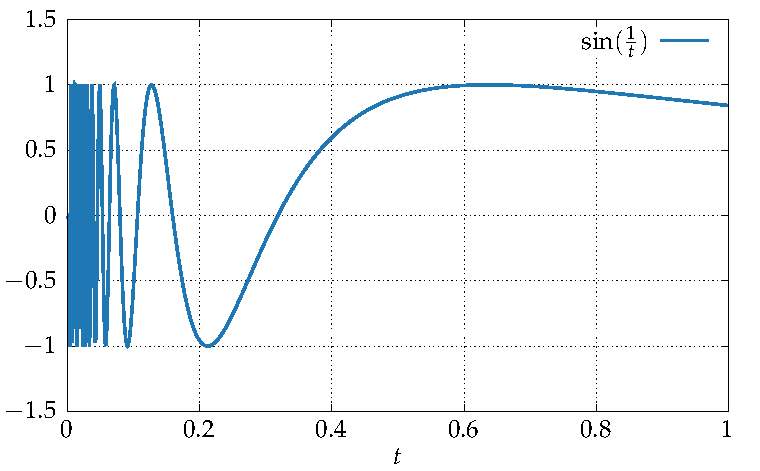
\includegraphics{gp_sininv.pdf}
  \caption{Curve of the function $f(t)=\sin(\frac{1}{t})$ from~\cref{ex:sininv}.}
  \label{fig:sininv}
\end{figure}
Finally, we show that the one-sided limits of the derivative of piecewise smooth functions
can be calculated with the usual limits:
\begin{proposition}
  \label{prop:oneside-der}
  Let $f$ be a piecewise smooth function on $[a,b]$, and let $t_0\in(a,b)$. The one-sided
  limits of $f'$ are given by the following limits
  \begin{equation}
    f'(t_0^-)=\lim_{\substack{h\to0\\h>0}}\frac{f(t_0^-)-f(t_0-h)}{h}
    \qquad\text{and}\qquad
    f'(t_0^+)=\lim_{\substack{h\to0\\h>0}}\frac{f(t_0+h)-f(t_0^+)}{h}
  \end{equation}
\end{proposition}
\begin{proof}
  Let $h>0$ small enough such that $t_0-h\in(a,b)$, and such that $f$ is continuously
  differentiable on $(t_0-h,t_0)$. Additionally, using condition (PC3)
  of~\cref{def:pw-cont}, $f$ restricted to $(t_0-h,t_0)$ can be extended to a continuous
  function on $[t_0-h,t_0]$ which take the value $f(t_0^-)$ in $t_0$. According to the
  mean value theorem, there exists $c_h$ in $(t_0-h,t_0)$ such that
  \begin{equation}
    f'(c_h)=\frac{f(t_0^-)-f(t_0-h)}{h}\,.
  \end{equation}
  Since $t_0-h<c_h<t_0$, then clearly $c_h\to t_0$ for $h\to 0$ with $h>0$, therefore
  \begin{equation}
    \lim_{\substack{h\to0\\h>0}}f'(c_h)=f'(t_0^-)
    =\lim_{\substack{h\to0\\h>0}}\frac{f(t_0^-)-f(t_0-h)}{h}\,.
  \end{equation}
  This proves the proposition for the left limit of $f'$. The right limit can be
  identically proven by considering the mean value theorem on a small interval
  $[t_0,t_0+h]$.
\end{proof}

%%%%%%%%%%%%%%%%%%%%%%%%%%%%%%%%%%%%%%%%%%%%%%%%%%%%%%%%%%%%%%%%%%%%%%%%%%%%%%%%%%%%%%%%%%
\section{Partial Fourier sums}
In this section, we formalise the generalisation of the
coefficients~\cref{eq:series-an-intro,eq:series-bn-intro,eq:series-cn-intro} mentioned in
the introduction to this section, as well as the associated trigonometric polynomials.
%.........................................................................................
\subsection{Fourier coefficients}
\begin{definition}
  \label{def:fourier-coef}
  Let $f$ be a piecewise smooth $\tau$-periodic function. We call \emph{cosine},
  \emph{sine}, and \emph{complex Fourier coefficients} the sequences
  \begin{align}
    a_n(f)&=\frac{2}{\tau}\braket{f,\cw(n\omega)}
    =\frac{2}{\tau}\int_0^{\tau}\diff t\,f(t)\cos(2\pi n\omega t)\,,\\
    b_n(f)&=\frac{2}{\tau}\braket{f,\sw(n\omega)}
    =\frac{2}{\tau}\int_0^{\tau}\diff t\,f(t)\sin(2\pi n\omega t)\,,\\
    c_n(f)&=\frac{1}{\tau}\braket{f,\ew(n\omega)}
    =\frac{1}{\tau}\int_0^{\tau}\diff t\,f(t)\,e^{-2\pi i n\omega t}\,,
  \end{align}
  respectively, where $n\in\mathbb{Z}$ and $\omega=\frac{1}{\tau}$.
\end{definition}
\begin{definition}
  \label{def:fourier-partial}
  Let $f$ be a piecewise smooth $\tau$-periodic function. For any integer $N\geq 0$, we
  call \emph{partial Fourier sum} of degree $N$ the trigonometric polynomial defined by
  \begin{equation}
    s_N(f)=\frac{a_0(f)}{2}+\sum_{n=1}^N[a_n(f)\cw(n\omega)+b_n(f)\sw(n\omega)]=
    \sum_{n=-N}^{N}c_n(f)\ew(n\omega)\,,
  \end{equation}
  where $\omega=\frac{1}{\tau}$.
\end{definition}
Since we aim at studying the convergence of Fourier sums for $N\to+\infty$, an important
question is the asymptotic behaviour of Fourier coefficients for $n\to+\infty$, discussed
in the next section.
%.........................................................................................
\subsection{Riemann-Lebesgue lemma}
For a fairly general class of functions, it can be shown that these coefficients converge
to $0$ for $n\to+\infty$. This is a crucial result in Fourier analysis generally called
the~\emph{Riemann-Lebesgue lemma}, and a necessary condition for the convergence of
Fourier series. We prove this result below for piecewise continuous functions on compact
intervals.
\begin{theorem}[Riemann-Lebesgue lemma]
  \label{thm:rl}
  Let $f$ be a piecewise continuous function on a compact interval $[a,b]$. We have the
  following limit
  \begin{equation}
    \lim_{k\to+\infty}\int_a^b\diff t\, f(t)\sin(kt)=0
  \end{equation}
\end{theorem}
\begin{proof}
  The proof of this theorem is rather abstract and technical, but it is based on a fairly
  intuitive idea. A first observation one can make is that the Riemann-Lebesgue lemma is
  easily demonstrated for constant functions. Indeed, for any constant $A\in\mathbb{R}$
  \begin{equation}
    \int_a^b\diff t\,A\sin(kt)=\frac{A}{k}\,[\cos(ka)-\cos(kb)]\,.
    \label{eq:rl-const}
  \end{equation}
  Then $|\cos(ka)-\cos(kb)|<2$ for all $k\in\mathbb{R}$, so the integral above clearly
  converges to $0$ for $k\to+\infty$. In the general case where $f$ is piecewise
  continuous, $f$ is an assembly of bounded continuous functions. Such functions can be
  approximated arbitrarily well by piecewise constant functions, similarly to what is done
  when approximating an integral with rectangles. With such a construction, the simple
  example above with constant functions is then all that is needed to prove the theorem.
  Let us proceed with justifying this approach in details.

  Reusing the notation of~\cref{def:pw-cont}, we have
  \begin{equation}
    \int_a^b\diff t\, f(t)\sin(kt)
    =\sum_{n=0}^{N}\int_{t_n}^{t_{n+1}}\diff t\, f(t)\sin(kt)\,.
    \label{eq:pw-int}
  \end{equation}
  The function $f$ is piecewise continuous, so according to condition (PC1)
  of~\cref{def:pw-cont}, for a given integer $n$ such that $0\leq n<N$, $f$ is continuous
  on $(t_n,t_{n+1})$. Additionally, conditions (PC2) and (PC3) imply that $f$ admits
  finite right and left limits in $t_n$ and $t_{n+1}$, respectively. Therefore, the
  restriction of $f$ to $(t_n,t_{n+1})$ can be extended to a continuous function on the
  compact interval $[t_n,t_{n+1}]$. Now, continuous functions on compact intervals are
  uniformly continuous, \ie for all $\epsilon>0$, there exists $\delta>0$ such that for
  all pairs $x,y$ in $[t_n,t_{n+1}]$, $|x-y|<\delta$ implies that $|f(x)-f(y)|<\epsilon$.
  Let us subdivide the interval $[t_n,t_{n+1}]$ into $M$ points
  $r_0=t_n<r_1<\dots<r_{M-1}<r_M=t_{n+1}$ such that for all $m$ with $0\leq m<M$,
  $|r_{n+1}-r_n|<\eta$. We then define the piecewise constant function $g$ equal to the
  constant $f(r_m)$ on $[r_m,r_{m+1})$, and $g(r_N)=f(r_{N-1})$. For a given point
  $t\in(t_n,t_{n+1})$, there exists $m$ such that $t\in[r_m,r_{m+1})$, and therefore
  \begin{equation}
    |f(t)-g(t)|=|f(t)-f(r_m)|<\epsilon\,,
  \end{equation}
  since by construction $|t-r_m|<\delta$. We can now write
  \begin{equation}
    \int_{t_n}^{t_{n+1}}\diff t\, f(t)\sin(kt)
    =\int_{t_n}^{t_{n+1}}\diff t\, [f(t)-g(t)]\sin(kt)
    +\int_{t_n}^{t_{n+1}}\diff t\,g(t)\sin(kt)\,.
  \end{equation}
  The integral of $g$ above can be dealt with easily, as anticipated in the introduction
  of the proof, explicitly
  \begin{equation}
    \int_{t_n}^{t_{n+1}}\diff t\,g(t)\sin(kt)
    =\frac{1}{k}\sum_{m=0}^{M-1}f(r_m)[\cos(kr_m)-\cos(kr_{m+1})]\,,
  \end{equation}
  so
  \begin{equation}
    \lim_{k\to0}\,\int_{t_n}^{t_{n+1}}\diff t\,g(t)\sin(kt)=0\,.
    \label{eq:rl-intg}
  \end{equation}
  Now, using the triangle inequality,
  \begin{equation}
    \left|\int_{t_n}^{t_{n+1}}\diff t\, [f(t)-g(t)]\sin(kt)\right|<
    \int_{t_n}^{t_{n+1}}\diff t\, |f(t)-g(t)|<(t_{n+1}-t_n)\epsilon\,.
  \end{equation}
  Since $\epsilon$ can be chosen arbitrarily small, the inequality above implies that
  \begin{equation}
    \lim_{k\to0}\,\int_{t_n}^{t_{n+1}}\diff t\, [f(t)-g(t)]\sin(kt)=0\,.
    \label{eq:rl-intfmg}
  \end{equation}
  Combining~\cref{eq:rl-intg,eq:rl-intfmg}, we just proved that every term in the sum
  in~\cref{eq:pw-int} converges to $0$ for $k\to+\infty$, which demonstrates the theorem.
\end{proof}
\begin{figure}[t]
  \centering
  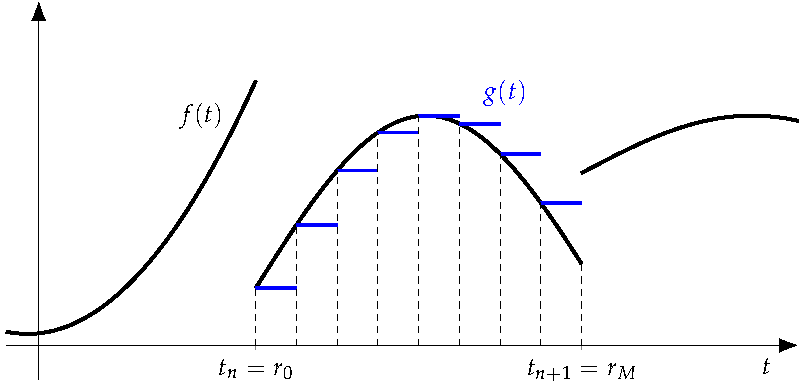
\includegraphics{tikz_rl.pdf}
  \caption{Illustration of the construction used in the proof of~\cref{thm:rl}
    (Riemann-Lebesgue lemma). The black curve represents an arbitrary piecewise continuous
    function, with visible jump discontinuities at $t_n$ and $t_{n+1}$. The blue lines
    represent a piecewise constant approximation $g$ of $f$ on the interval
  $[t_n,t_{n+1}]$, as defined in the proof of~\cref{thm:rl}}
  \label{fig:rl}
\end{figure}
\begin{corollary}
  Let $f$ be a function on $\mathbb{R}$ piecewise smooth on a compact interval $[a,b]$. We
  have the following limits
  \begin{align}
    \lim_{k\to+\infty}\int_a^b\diff t\, f(t)\cos(kt)&=0\,,\\
    \lim_{k\to+\infty}\int_a^b\diff t\, f(t)\,e^{ikt}=0
  \end{align}
\end{corollary}
\begin{proof}
  One can inspect the proof of~\cref{thm:rl} and notice that the only dependency on the
  $\sin(kt)$ weight in the integral comes from~\cref{eq:rl-const}. So it is sufficient to
  just repeat that step for the cosine function. We have
  \begin{equation}
    \int_a^b\diff t\, f(t)\cos(kt)=\frac{1}{k}[\sin(bk)-\sin(ak)]\,,
  \end{equation}
  and since $|\sin(bk)-\sin(ak)|<2$ for all $k\in\mathbb{R}$, the integral above vanishes
  for $k\to+\infty$. A similar argument can be made for the complex exponential, although
  one can also notice that it is now a trivial consequence the equality
  \begin{equation}
    \int_a^b\diff t\, f(t)\,e^{ikt}
    =\int_a^b\diff t\, f(t)\cos(kt)+i\int_a^b\diff t\, f(t)\sin(kt)\,.
  \end{equation}
\end{proof}
\begin{corollary}
  Let $f$ be a piecewise smooth $\tau$-periodic function. All the Fourier coefficients of
  $f$ converge to $0$, explicitly
  \begin{equation}
    \lim_{n\to+\infty}a_n(f)=\lim_{n\to+\infty}b_n(f)=\lim_{n\to+\infty}c_n(f)=0\,.
  \end{equation}
\end{corollary}
\begin{proof}
  This is a trivial consequence of the Riemann-Lebesgue lemma applied
  to~\cref{def:fourier-coef}.
\end{proof}
%.........................................................................................
\subsection{Dirichlet kernel}
In this section, we discuss a special function called the \emph{Dirichlet kernel}. This
function allows to write the partial Fourier sums as an integral (and as we will see in
later chapters, a convolution product), which is often used in combination with the
Riemann-Lebesgue lemma to demonstrate theorems on the convergence of Fourier series.
\begin{definition}
  We call~\emph{Dirichlet kernel} of degree $N$ the trigonometric polynomial defined by
  \begin{equation}
    D_N(x)=\sum_{n=-N}^{N}e^{inx}\,,\label{eq:dk-def}
  \end{equation}
  for any real number $x$. The Dirichlet kernel is by construction even and periodic with
  fundamental period $2\pi$.
\end{definition}
The Dirichlet kernel can in fact be expressed as a simple ratio of sine functions as
discussed in the result below.
\begin{proposition}
  \label{prop:dirichlet-id}
  For all $x\in\mathbb{R}$, and all $N\in\mathbb{N}$, we have
  \begin{equation}
    D_N(x)=1+2\sum_{n=1}^{N}\cos(nx)=\frac{\sin[(N+\frac{1}{2})x]}{\sin(\frac{x}{2})}\,.
    \label{eq:dk-sinratio}
  \end{equation}
\end{proposition}
\begin{proof}
  We start by defining the complex number $z$ by
  \begin{equation}
    z=\sum_{n=0}^Ne^{inx}\,.
  \end{equation}
  The Dirichlet kernel can then be written as follows:
  \begin{equation}
    D_N(x)=(z-1)^*+z=z^*+z-1=2\Re(z)-1=1+2\sum_{n=1}^{N}\cos(nx)\,,\label{eq:dk-z}
  \end{equation}
  which proves the first equality in~\cref{eq:dk-sinratio}. Since $e^{inx}=(e^{ix})^n$, we
  can simplify $z$ using a geometric sum:
  \begin{equation}
    z=\frac{e^{i(N+1)x}-1}{e^{ix}-1}\,.\label{eq:dk-geosum}
  \end{equation}
  We now have to compute the real part of $z$, let us start by rewriting the equation
  above to have a real denominator:
  \begin{equation}
    z=e^{-i\frac{x}{2}}\frac{e^{i(N+1)x}-1}{e^{i\frac{x}{2}}-e^{-i\frac{x}{2}}}
    =\frac{e^{i(N+\frac12)x}-e^{-i\frac{x}{2}}}{2i\sin(\frac{x}{2})}
    =-\frac{i}{2}\frac{e^{i(N+\frac12)x}-e^{-i\frac{x}{2}}}{\sin(\frac{x}{2})}\,,
  \end{equation}
  which has the real part
  \begin{equation}
    \Re(z)=\frac12\frac{\Im[e^{i(N+\frac12)x}]-\Im(e^{-i\frac{x}{2}})}{\sin(\frac{x}{2})}
    =\frac12\frac{\sin[(N+\frac{1}{2})x]}{\sin(\frac{x}{2})}+1\,.
  \end{equation}
  Substituting the last equation into~\cref{eq:dk-z} proves the proposition.
\end{proof}
\begin{proposition}
  \label{prop:dk-int}
  The Dirichlet kernel has the following integral on $[0,2\pi]$ for all $N\in\mathbb{N}$:
  \begin{equation}
    \int_0^{2\pi}\diff x\,D_N(x)=2\pi\,.
  \end{equation}
\end{proposition}
\begin{proof}
  Using~\cref{thm:orth-complex} with $m=0$ and $\tau=2\pi$, we obtain
  \begin{equation}
    \int_{0}^{2\pi}\diff x\,e^{inx}=2\pi\,\delta_{n0}\,,
  \end{equation}
  which substituted into~\cref{eq:dk-def} directly proves the proposition.
\end{proof}
We now formulate the main theorem on the integral representation of partial Fourier sums.
\begin{theorem}
  \label{thm:fourier-dk-rep}
  Let $f$ be a piecewise smooth $\tau$-periodic function. For all $N\in\mathbb{N}$, the
  partial Fourier sum of $f$ has the following integral representation:
  \begin{equation}
    s_N(f)(t)=\frac{1}{\tau}\int_0^{\tau}\diff u\,f(u)\,D_N[2\pi\omega(t-u)]\,.
  \end{equation}
\end{theorem}
\begin{proof}
  Using~\cref{def:fourier-coef,def:fourier-partial}, the partial Fourier sum $s_N(f)$ is
  given by
  \begin{equation}
    s_N(f)(t)=\frac{1}{\tau}\sum_{n=-N}^{N}e^{2\pi i n\omega t}
    \int_0^\tau\diff u\,f(u)e^{-2\pi i n\omega u}\,.
  \end{equation}
  Since the sum above is finite, we can exchange the sum and the integral to obtain
  \begin{equation}
    s_N(f)(t)=\frac{1}{\tau}\int_0^\tau\diff u\,f(u)\sum_{n=-N}^{N}e^{2\pi i n\omega (t-u)}\,.
  \end{equation}
  Finally, using the definition of the Dirichlet kernel~\cref{eq:dk-def} proves the
  theorem.
\end{proof}
%%%%%%%%%%%%%%%%%%%%%%%%%%%%%%%%%%%%%%%%%%%%%%%%%%%%%%%%%%%%%%%%%%%%%%%%%%%%%%%%%%%%%%%%%%
\section{Convergence of the Fourier expansion}
Using results from the previous section, we are now ready to discuss in details the
convergence of Fourier series. We start by discussing pointwise convergence, in a context
close to the original work of Peter Gustav Lejeune Dirichlet and Camille Jordan in the
second half of the 19\textsuperscript{th}, who brought stronger mathematical foundations
to the pioneering work of Fourier. We will then discuss the much stronger case of uniform
convergence, and conclude the section with the Gibbs phenomenon, which describes important
practical consequences of Fourier series which fail to converge uniformly.
%-----------------------------------------------------------------------------------------
\subsection{Pointwise convergence}
The theorem below can be considered as the main result of this chapter. It states that for
piecewise smooth periodic functions, the Fourier series converges at every point to the
average of the left and right limits. The essence of this theorem is that the Fourier
series does converge back to a given piecewise smooth periodic function, expect perhaps at
a finite number of points of jump discontinuity.
\begin{theorem}
  \label{thm:fourier-pt}
  Let $f$ be a $\tau$-periodic function which is piecewise smooth on $[0,\tau]$. For all
  $t\in\mathbb{R}$, the Fourier series for $f(t)$ converges with the following limit
  \begin{equation}
    \sumz{n}c_n(f)\,e^{2\pi i \omega nt}=\lim_{N\to+\infty}s_N(f)(t)
    =\frac{f(t^-)+f(t^+)}{2}\,.
  \end{equation}
  In particular, the Fourier series converges to $f(t)$ if $f$ is continuous in $t$.
\end{theorem}
\begin{proof}
  Let $t$ be a point in $[0,\tau]$. Using~\cref{thm:fourier-dk-rep}, we can write the
  partial Fourier sum $s_N(f)$ at the point $t$ as
  \begin{equation}
    s_N(f)(t)=\frac{1}{\tau}\int_{-\frac{\tau}{2}}^{\frac{\tau}{2}}\diff u\,
    f(u)\,D_N[2\pi\omega(t-u)]\,,
  \end{equation}
  where $\omega=\frac{1}{\tau}$, and the integration domain was shifted to
  $(-\frac{\tau}{2},\frac{\tau}{2})$, which is allowed by the $\tau$-periodicity of the
  integrand. We additionally perform the change of variable $u\mapsto t-u$ to obtain
  \begin{equation}
    s_N(f)(t)=\frac{1}{\tau}\int_{-\frac{\tau}{2}}^{\frac{\tau}{2}}\diff u\,
    f(t-u)\,D_N(2\pi\omega u)\,.
  \end{equation}
  Now, using~\cref{prop:dk-int}, we get
  \begin{equation}
    \int_{-\frac{\tau}{2}}^{\frac{\tau}{2}}\diff u\,D_N(2\pi\omega u)
    =\frac{\tau}{2\pi}\int_{-\pi}^{\pi}\diff x\,D_N(x)=
    \frac{\tau}{2\pi}\int_{0}^{2\pi}\diff x\,D_N(x)=\tau\,,
    \label{eq:fthm-partsum}
  \end{equation}
  where we used the change of variable $x=2\pi\omega u$, as well as the $2\pi$-periodicity
  of the Dirichlet kernel. Similarly, since $D_N(x)$ is even, we can write
  \begin{equation}
    \int_{0}^{\frac{\tau}{2}}\diff u\,D_N(2\pi\omega u)
    =\int_{-\frac{\tau}{2}}^{0}\diff u\,D_N(2\pi\omega u)=\frac{\tau}{2}\,.
  \end{equation}
  Since $f(t^-)$ and $f(t^+)$ are just constants, we can write
  \begin{align}
    \frac{f(t^-)}{2}&=\frac{1}{\tau}\int_{0}^{\frac{\tau}{2}}\diff u\,
    f(t^-)D_N(2\pi\omega u)\,,
    \label{eq:fthm-tmint}\\
    \frac{f(t^+)}{2}&=\frac{1}{\tau}\int_{-\frac{\tau}{2}}^{0}\diff u\,
    f(t^+)D_N(2\pi\omega u)\,.
    \label{eq:fthm-tpint}
  \end{align}
  We consider the two following integrals
  \begin{align}
    I^-_N&=\frac{1}{\tau}\int_{0}^{\frac{\tau}{2}}\diff u\,
    [f(t-u)-f(t^-)]D_N(2\pi\omega u)\,,\\
    I^+_N&=\frac{1}{\tau}\int_{-\frac{\tau}{2}}^{0}\diff u\,
    [f(t-u)-f(t^+)]D_N(2\pi\omega u)\,.
  \end{align}
  Using~\cref{eq:fthm-partsum,eq:fthm-tmint,eq:fthm-tpint}, we get
  \begin{equation}
    I^-_N+I^+_N=s_N(f)(t)-\frac{f(t^-)+f(t^+)}{2}\,.
    \label{eq:fourier-imip}
  \end{equation}
  Therefore, if we can show that $I^-_N$ and $I^+_N$ converge to $0$ for $N\to+\infty$,
  then the theorem is proven. Let us start by discussing $I^-_N$.
  Using~\cref{prop:dirichlet-id}, we can write
  \begin{equation}
    I^-_N=\frac{1}{\tau}\int_{0}^{\frac{\tau}{2}}\diff u\,
    \varphi^-(u)\sin\left[\left(N+\frac{1}{2}\right)2\pi\omega u\right]\,,
  \end{equation}
  where $\varphi^-$ is the function defined on all $u\in(0,\frac{\tau}{2})$ by
  \begin{equation}
    \varphi^-(u)=\frac{f(t-u)-f(t^-)}{\sin(\pi\omega u)}
    =\frac{f(t-u)-f(t^-)}{u}\frac{u}{\sin(\pi\omega u)}\,.
  \end{equation}
  If we can prove that $\varphi^-$ is piecewise continuous on
  $\smash{[0,\frac{\tau}{2}]}$, then $I^-_N$ converging to zero for $N\to+\infty$ is a
  direct consequence of the Riemann-Lebesgue lemma. Since $\sin(\pi\omega u)\neq 0$ for
  all $u\in\smash{(0,\frac{\tau}{2}]}$, and $f$ is piecewise smooth, the formula above
  clearly satisfies conditions (PC1) and (PC2) of~\cref{def:pw-cont}. However, it has an
  apparent singularity at $u=0$ that needs to be discussed for (PC3) to hold. For $u\to
  0$, $\sin(\pi\omega u)=\pi\omega u+\mathcal{O}(u^2)$ and therefore
  \begin{equation}
    \lim_{u\to 0}\,\frac{u}{\sin(\pi\omega u)}=\frac{1}{\pi\omega}\,.
  \end{equation}
  Then, using~\cref{prop:oneside-der}, we obtain
  \begin{equation}
    \lim_{\substack{u\to0\\u>0}}\varphi^-(u)=-\frac{f'(t^-)}{\pi\omega}\,,
  \end{equation}
  So $\varphi^-$ has a well-defined right limit for $u\to 0$, condition (PC3) is
  satisfied, $\varphi^-$ is piecewise continuous on $\smash{[0,\frac{\tau}{2}]}$,
  and~\cref{thm:rl} implies that
  \begin{equation}
    \lim_{N\to+\infty}I^-_N=0\,.
  \end{equation}
  We similarly write $I_N^+$ as
  \begin{equation}
    I^+_N=\frac{1}{\tau}\int_{-\frac{\tau}{2}}^{0}\diff u\,
    \varphi^+(u)\sin\left[\left(N+\frac{1}{2}\right)2\pi\omega u\right]\,,
  \end{equation}
  where
  \begin{equation}
    \varphi^+(u)=\frac{f(t-u)-f(t^+)}{\sin(\pi\omega u)}\,.
  \end{equation}
  As above, the limit
  \begin{equation}
    \lim_{\substack{u\to0\\u<0}}\varphi^+(u)=\frac{f'(t^+)}{\pi\omega}
  \end{equation}
  shows that $\varphi^+$ is piecewise continuous on $\smash{[-\frac{\tau}{2},0]}$, and
  therefore
  \begin{equation}
    \lim_{N\to+\infty}I^+_N=0\,.
  \end{equation}
  Coming back to~\cref{eq:fourier-imip}, the theorem is proven.
\end{proof}
\begin{example}
  The Fourier series of the square wave $\sq$ defined in~\cref{eq:wave-square} converges
  to the function
  \begin{equation}
    \sumz{n}c_n(\sq)\,e^{2\pi i \omega nt}=
    \begin{cases}
      1&\text{if}~0<t<\frac{1}{2}\\
      -1&\text{if}~\frac{1}{2}<t<-1\\
      \frac{1}{2}&\text{if}~t=0,\frac{1}{2},1
    \end{cases}\,,
  \end{equation}
  where it is understood that these values are repeated on every period. This limit is
  identical to the square wave except at the points of discontinuity where it takes the
  value $\frac{1}{2}$.
\end{example}
%-----------------------------------------------------------------------------------------
\subsection{Convergence in mean square and Parseval's theorem}
Another useful form of convergence for sequences of functions is the \emph{convergence in mean square}, also called \emph{$L^2$ convergence}, based on the functional norm introduced in~\cref{sec:ew-orth}. In all this section, we will work with square-integrable $\tau$-periodic functions. Such a function $f$ is defined by requiring that $|f|^2$ has a defined finite integral on $[0,\tau]$. This is the general class of functions for which the dot product is well-defined, which we will admit here. In particular, all piecewise smooth functions are square-integrable.
\begin{definition}
  Let $f$ be a $\tau$-periodic square-integrable function. A sequence of $\tau$-periodic square-integrable functions $f_n$ is said to converge to $f$ \emph{in mean} if
  \begin{equation}
    \lim_{n\to+\infty}\|f-f_n\|=0\,.
  \end{equation}
\end{definition}
This type of convergence is useful because the norm is related to the dot product of functions,
and as we saw in the previous chapter, the orthogonality of elementary waves. However, it is important to notice that this is a rather weak form of convergence, and without further assumptions it does not generally imply pointwise or uniform convergence.

We now generalise some results of~\cref{sec:ew-orth}, which we will then use to prove that Fourier series generally converge in mean square. Firstly, it is not too difficult to
show that the norm of a partial Fourier sum is always smaller than the norm of the associated function,
an important result known as \emph{Bessel's inequality}.
\begin{theorem}[Bessel's inequality]
  \label{thm:bessel}
  Let $f$ be a piecewise smooth $\tau$-periodic function. The series over $n\in\mathbb{Z}$
  with summand $|c_n(f)|^2$ converges, and one has the inequality
  \begin{equation}
    \tau\sumz{n}|c_n(f)|^2\leq\|f\|^2\,.
  \end{equation}
\end{theorem}
\begin{proof}
  We consider the norm of the difference between $f$ and its partial Fourier sum
  \begin{equation}
    \Delta_N=\|f-s_N(f)\|^2\,,
  \end{equation}
  where $N$ is some positive integer. By construction, $\Delta_N\geq 0$ for all $N>0$.
  Additionally, $\Delta_N$ can be expanded as
  \begin{align}
    \Delta_N&=\braket{f-s_N(f),f-s_N(f)}\\
    &=\|f\|^2+\|s_N(f)\|^2-2\Re[\braket{f,s_N(f)}]\,.\label{eq:bessel-l2err}
  \end{align}
  Furthermore,
  \begin{align}
    \braket{f,s_N(f)}&=\Braket{f,\sum_{n=-N}^{N}c_n(f)\ew(n\omega)}\\
    &=\sum_{n=-N}^{N}c_n(f)^*\braket{f,\ew(n\omega)}\\
    &=\tau\sum_{n=-N}^{N}|c_n(f)|^2\,.
  \end{align}
  Using Parseval's theorem for trigonometric polynomials (\cref{thm:trigp-parseval}), the result
  above implies that $\braket{f,s_N(f)}=\|s_N(f)\|^2$. Substituting this expression back into
  \cref{eq:bessel-l2err}, we get
  \begin{equation}
    \Delta_N=\|f\|^2-\|s_N(f)\|^2\,,
  \end{equation}
  and since $\Delta_N\geq 0$,
  \begin{equation}
    \forall N>0,\quad \|s_N(f)\|^2=\tau\sum_{n=-N}^{N}|c_n(f)|^2\leq \|f\|^2\,.
  \end{equation}
  $\|s_N(f)\|^2$ is a sum of positive numbers, and therefore a monotonous sequence in $N$. As per the inequality above, it is bounded by $\|f\|^2$ and therefore converges, which proves the theorem.
\end{proof}
In reality, this inequality is an equality, generalising~\cref{thm:trigp-parseval}. This is a much harder result to prove, and we will admit it here.
\begin{theorem}[Parseval]
  \label{thm:parseval}
  Let $f$ and $g$ be two square-integrable $\tau$-periodic functions. The following identities hold
  \begin{align}
    \braket{f,g}&=\tau\sumz{n}c_n(f)c_n(g)^*\,,
    \label{eq:fs-dot}\\
    \|f\|^2&=\tau\sumz{n}|c_n(f)|^2\,.
    \label{eq:fs-norm}
  \end{align}
\end{theorem}
For completeness, we provide below the Parseval theorem identities for the sine-cosine form
\begin{align}
  \braket{f,g}&=\tau\,\frac{a_0(f)a_0(g)^*}{4}
  +\frac{\tau}{2}\left\{\sumnp{n}[a_n(f)a_n(g)^*+b_n(f)b_n(g)^*]\right\}\,,\\
  \|f\|^2&=\tau\,\frac{|a_0(f)|^2}{4}+\frac{\tau}{2}\left\{\sumnp{n}[|a_n(f)|^2+|b_n(f)|^2]\right\}\,.
\end{align}
\begin{theorem}
  Let $f$ be a square-integrable $\tau$-periodic function. The Fourier series of $f$
  converges to $f$ in mean.
\end{theorem}
\begin{proof}
  We need to show that
  \begin{equation}
    \Delta_N =\|f-s_N(f)\|^2
  \end{equation}
  converges to $0$ for $N\to+\infty$. As already demonstrated in the proof of~\cref{thm:bessel},
  \begin{equation}
    \Delta_N =\|f\|^2-\tau\sum_{n=-N}^{N}|c_n(f)|^2\,.\label{eq:l2cvg-deltan}
  \end{equation}
  Using Parseval's theorem, we know that
  \begin{equation}
    \lim_{N\to+\infty}\tau\sum_{n=-N}^{N}|c_n(f)|^2=\|f\|^2\,,
  \end{equation}
  which applied to~\cref{eq:l2cvg-deltan} proves the theorem.
\end{proof}
The proof above is quite simple once one knows Parseval's theorem. In fact, Parseval's theorem
is truly the non-trivial property here, and it can be shown to be a necessary and sufficient condition
to the convergence in mean square. Proving Parseval's theorem it quite technical and out of the scope of this introductory course, however we will sketch the proof in the next section.
\subsection{Uniform convergence}
We start by reminding the definition of uniform convergence for a sequence of functions.
Essentially, such sequence is uniformly convergent if the distance to the limit can be
bounded independently of the point at which the function is evaluated, as formalised in
the definition below.
\begin{definition}
  A sequence of function $f_n$ is said to \emph{converge uniformly} to $f$ on a domain $D$
  if for all $\epsilon>0$, there exists $N\in\mathbb{N}$ such that
  \begin{equation}
    \forall n\geq N,\quad\forall x\in D,\quad|f_n(x)-f(x)|<\epsilon\,,
  \end{equation}
  which can equivalently be defined as the limit
  \begin{equation}
    \lim_{n\to+\infty}\,\sup_{x\in D}|f_n(x)-f(x)|=0\,.
  \end{equation}
\end{definition}
\begin{example}
  The sequence of functions defined by $\sin(t+\frac{1}{n})$ converges uniformly to
  $\sin(t)$ in the $n\to+\infty$ limit. Indeed,
  \begin{equation}
    \sin\left(t+\frac{1}{n}\right)-\sin(t)
    =2\sin\left(\frac{1}{2n}\right)\cos\left(t+\frac{1}{2n}\right)\,,
  \end{equation}
  therefore
  \begin{equation}
    \sup_{t\in\mathbb{R}}\left|\sin\left(t+\frac{1}{n}\right)
    -\sin(t)\right|=2\sin\left(\frac{1}{2n}\right)\,.
  \end{equation}
  The right-hand side of the equation above converges to $0$ for $n\to+\infty$, which
  proves the uniform convergence.
\end{example}
\begin{example}
  The sequence of functions defined by $t^n$ converges uniformly to $0$ on any interval of
  the form $[0,a]$ with $a<1$, but not on $[0,1)$. Indeed, for $t\in [0,1)$, clearly
  \begin{equation}
    \lim_{n\to+\infty}t^n=0\,,
  \end{equation}
  so $t^n$ converges pointwise to $0$ on $[0,1)$. Let $a\in(0,1)$, since $t^n$ is a
  positive, increasing function for $t>0$, we have
  \begin{equation}
    \sup_{t\in[0,a]}|t^n|=a^n\,,
  \end{equation}
  and since $a<1$,
  \begin{equation}
    \lim_{n\to+\infty}\sup_{t\in[0,a]}t^n=0\,,
  \end{equation}
  so $t^n$ converges uniformly to $0$ on $[0,a]$. However,
  \begin{equation}
    \sup_{t\in[0,1)}|t^n|=1\,,
  \end{equation}
  so $t^n$ does not converge uniformly to $0$ on $[0,1)$.
\end{example}
\begin{theorem}
  Let $f$ be a $\tau$-periodic function which is piecewise smooth and continuous on
  $[0,\tau]$. The Fourier series of $f$ converges uniformly to $f$.
\end{theorem}
\subsection{Gibbs phenomenon}
If a periodic function has a jump discontinuity, then its Fourier series cannot be
uniformly convergent. This generates irregularities around discontinuities where the
Fourier expansion tends to ``overshoot'' the function by approximately $9\%$ of the height
of the discontinuity. This effect is generally called the \emph{Gibbs phenomenon}, and is
a well known engineering issue when cutting data before computing its Fourier
coefficients. A key example of Gibbs phenomenon is the Fourier expansion of the square
wave.
\begin{lemma}
  \label{lem:gibbs-sq}
  The square wave Fourier series does not converge uniformly on $[0,1]$, and
  \begin{align}
    \lim_{N\to+\infty}\,s_N(\sq)\left(\frac12-\frac{1}{2N}\right)
    &=1+2\left(\frac{G'}{\pi}-\frac12\right)\,,\label{eq:gibbs-sq-left}\\
    \lim_{N\to+\infty}\,s_N(\sq)\left(\frac12+\frac{1}{2N}\right)
    &=-1-2\left(\frac{G'}{\pi}-\frac12\right)\,,
  \end{align}
  where $G'$ is the \emph{Wilbraham-Gibbs constant} given by
  \begin{equation}
    G'=\int_0^\pi\diff t\,\frac{\sin(t)}{t}\simeq1.851937052\dots\,.
  \end{equation}
\end{lemma}
\begin{proof}
  A guided proof is available as an exercise in Problem~\ref{gibbs}.
\end{proof}
\begin{figure}[t]
  \centering
  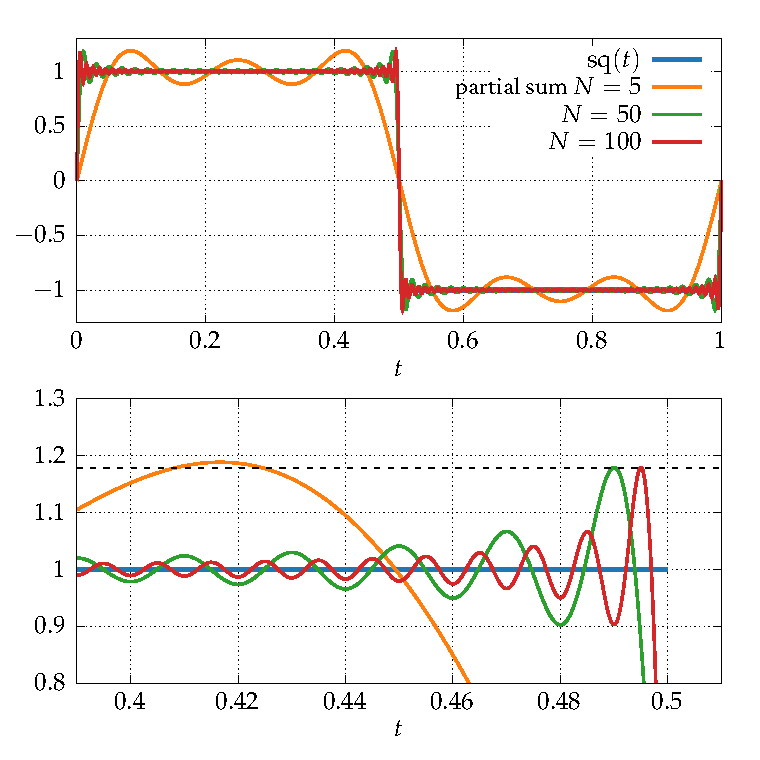
\includegraphics{gp_gibbs-sq.pdf}
  \caption{Gibbs phenomenon in the Fourier expansion of the square wave. The upper pane
    represents the square wave on one period, and its partial Fourier sum for various
    degrees. The lower pane is a zoom on the region close to the jump discontinuity at
  $t=\frac12$, and the dashed line is the excess predicted by~\cref{eq:gibbs-sq-left}.}
  \label{fig:gibbs-sq}
\end{figure}
The Fourier expansion of the square wave is illustrated in~\cref{fig:gibbs-sq}, where the
Gibbs phenomenon is clearly visible. The Gibbs phenomenon for the square wave can be
generalised to arbitrary discontinuous piecewise smooth functions, as summarised in the
theorem below.
\begin{theorem}[Gibbs phenomenon]
  Let be a $\tau$-periodic function which is piecewise smooth on $[0,\tau]$, which has a
  jump discontinuity of height $d$ at $t_0\in(0,\tau)$. Let $[a,b]$ be a sub-interval of
  $[0,\tau]$ such that $t_0\in(a,b)$, and $t_0$ is the only jump discontinuity of $f$ in
  $[a,b]$. The Fourier series of $f$ does not converge uniformly to $f$ on $[a,b]$, and
  \begin{align}
    \lim_{N\to+\infty}\,s_N(f)\left(t_0-\frac{\tau}{2N}\right)
    &=f(t_0^-)-d\left(\frac{G'}{\pi}-\frac12\right)\,,\\
    \lim_{N\to+\infty}\,s_N(f)\left(t_0+\frac{\tau}{2N}\right)
    &=f(t_0^+)+d\left(\frac{G'}{\pi}-\frac12\right)\,,
  \end{align}
  where $G'$ is the Wilbraham-Gibbs constant defined in~\cref{lem:gibbs-sq}.
\end{theorem}
%%%%%%%%%%%%%%%%%%%%%%%%%%%%%%%%%%%%%%%%%%%%%%%%%%%%%%%%%%%%%%%%%%%%%%%%%%%%%%%%%%%%%%%%%%
\section{Properties of Fourier coefficients}
%%%%%%%%%%%%%%%%%%%%%%%%%%%%%%%%%%%%%%%%%%%%%%%%%%%%%%%%%%%%%%%%%%%%%%%%%%%%%%%%%%%%%%%%%%
\section{Multidimensional Fourier series}

\vfill\pagebreak
% !TEX root = ../waves.tex
%%%%%%%%%%%%%%%%%%%%%%%%%%%%%%%%%%%%%%%%%%%%%%%%%%%%%%%%%%%%%%%%%%%%%%%%%%%%%%%%%%%%%%%%%%
\section{Exercises}
\begin{ExerciseList}
  %---------------------------------------------------------------------------------------
  \Exercise[label=seriesex]~
  \Question Compute the Fourier coefficients of the functions below. All functions are assumed periodic, and the given interval represents one period.
  \subQuestion $f(t)=t^2$, on $[-\pi,\pi]$.
  \subQuestion $f(t)=t^2$, on $[0,2\pi]$.
  \subQuestion $f(t)=\cos(\alpha t)$, where $\alpha\in\R$ is not an integer, on $[-\pi,\pi]$.
  \subQuestion $f(t)=|\sin(t)|^3$ (determine the fundamental period).
  \Question Using the result of question 1.c, show that if $t\in\R$ is not an integer multiple of $\pi$,
  \begin{equation}
    \frac{1}{\tan(t)}=\frac{1}{t}+\sumnp{n}\frac{2t}{t^2-n^2\pi^2}\,.\label{eq:cotan-sing}
  \end{equation}
  \Question Using the result of question 1.d, show that
  \begin{equation}
    \pi^2=\frac{256}{45}+\frac{4608}{5}\sumnp{n}\frac{1}{(4n^2-1)^2(4n^2-9)^2}\,.\label{eq:hard-pi2}
  \end{equation}
  %---------------------------------------------------------------------------------------
  \Exercise[label=fourierode2] Let $f$ be a real twice and continuously differentiable function on $\R$ which is
  a solution of the ordinary differential equation
  \begin{equation}
    f''(t) + A f(t) = 0\,,\label{eq:fourierode2}
  \end{equation}
  where $A\in\R$. We additionally assume that $f$ is $\tau$-periodic.
  \Question Using Fourier series, show that if $f\neq 0$ then $A\geq 0$.
  \Question If $A\geq 0$, show that there exists two real numbers $a$ and $b$
  such that
  \begin{equation}
    f(t)=a\cos(\sqrt{A} t)+b\sin(\sqrt{A} t)\,.
  \end{equation}
  %---------------------------------------------------------------------------------------
  \Exercise[label=seriesdecay]~
  Let $f$ be the periodic function defined by $f(t)=|\sin(t)|^3$. What is the expected
  decay rate for the Fourier coefficients of $f$? Compare this expectation with the
answer of question 1.d) in~\cref{seriesex}.
%---------------------------------------------------------------------------------------
\Exercise[label=seriessmooth]~
Let $f$ be the $2\pi$-periodic function defined by
\begin{equation}
  f(t)=\frac{1-p\cos(t)}{1+p^2-2p\cos(t)}\,,
\end{equation}
with $p\in(-1,1)$.
\Question Show that
\begin{equation}
  f(t)=\Re\left[\frac{1}{1-pe^{-it}}\right]\,.
\end{equation}
\Question Deduce the Fourier series of $f$ from the answer to the previous question.
\pagebreak
\InputIfFileExists{solutions/series}{}{}
\end{ExerciseList}

\shipoutAnswer
\vfill\pagebreak
% !TEX root = ../waves.tex
%%%%%%%%%%%%%%%%%%%%%%%%%%%%%%%%%%%%%%%%%%%%%%%%%%%%%%%%%%%%%%%%%%%%%%%%%%%%%%%%%%%%%%%%%%
\begin{Exercise}[title={Gibbs Phenomenon for the square wave},name={Problem},label=gibbs]
  We remind that the \emph{square wave} function $\sq$ is the function of period $1$ defined
  for $t\in[0,1)$ by
  \begin{equation}
    \sq(t)=
    \begin{cases}
      1&\text{if}~0\leq t <\frac{1}{2}\\
      -1&\text{if}~\frac{1}{2}\leq t < 1
    \end{cases}\,.
  \end{equation}
  This function was previously defined in~\cref{eq:wave-square} and illustrated
  in~\cref{fig:sq-wave}.
  \Question Show that the square wave Fourier coefficients are given by
  \begin{align}
    a_n(\sq)&=2\int_0^1\diff t\,\sq(t)\cos(2\pi nt)=0\,,\\
    b_n(\sq)&=2\int_0^1\diff t\,\sq(t)\sin(2\pi nt)=
    \begin{cases}
      0&\text{if}~$n$~\text{is even}\\
      \frac{4}{\pi n}&\text{if}~$n$~\text{is odd}
    \end{cases}\,,
  \end{align}
  for all $n\in\mathbb{N}$.
  \Question Show that, for all $M\in\mathbb{N}$ and $t\in\mathbb{R}$ such that $\sin(2\pi t)\neq 0$,
  \begin{equation}
    \sum_{n=0}^{M-1}\cos[2\pi(2n+1)t]=\frac{\sin(4\pi Mt)}{2\sin(2\pi t)}\,.
  \end{equation}
  \emph{Hint: review the proof of~\cref{prop:dirichlet-id}.}
  \Question Extend the result of the previous question for the cases when $\sin(2\pi t)=0$.
  \Question We consider the partial Fourier sum of the square wave
  \begin{equation}
    s_{N}(\sq)(t)=\sum_{n=1}^N b_n(\sq)\sin(2\pi n t)=\sum_{n=0}^{M-1}\frac{4}{\pi(2n+1)}\sin[2\pi(2n+1)t]\,,
  \end{equation}
  with $N$ is assumed to be even and $M=\frac{N}{2}$.
  \subQuestion Show that the derivative in $t$ of $s_{N}(\sq)(t)$ is given by
  \begin{equation}
    s_{N}(\sq)'(t)=\frac{4\sin(4\pi Mt)}{\sin(2\pi t)}
  \end{equation}
  \subQuestion Show that $s_{N}(\sq)'(t)=0$ for $t=t_k$ with $t_k=\frac{k}{4M}$,
  where $k$ is any integer which is not a multiple of $2M$.
  \subQuestion Show that, for $1\leq k \leq 2M-1$, $t_k$ is a local maximum of $s_{N}(\sq)$ if $k$ is odd, and a local
  minimum if $k$ is even.
  \subQuestion We consider the local maximum at $t_{2M-1}=\smash{\frac{1}{2}-\frac{1}{4M}}=\smash{\frac{1}{2}-\frac{1}{2N}}$, the closest to the jump discontinuity of $\sq(t)$ at $t=\frac12$. Show that
  \begin{equation}
    s_{N}(\sq)(t_{2M-1})=\frac{2}{M}\sum_{n=0}^{M-1}\frac{2M}{\pi(2n+1)}\sin\left[\frac{\pi(2n+1)}{2M}\right]\,.
  \end{equation}
  \subQuestion Prove~\cref{eq:gibbs-sq-left} from~\cref{lem:gibbs-sq}, \ie
  \begin{equation}
    \lim_{N\to+\infty} s_{N}(\sq)\left(\frac{1}{2}-\frac{1}{2N}\right)=
    \frac{2}{\pi}\int_0^{\pi}\diff x\,\frac{\sin(x)}{x}\simeq 1+0.18\,.
  \end{equation}
  \emph{Hint: Remember the mid-point rule}
  \begin{equation}
    \int_0^1\diff t\,f(t)=\lim_{M\to+\infty}\frac{1}{M}\sum_{n=0}^{M-1}f\left(\frac{2n+1}{2M}\right)\,.
  \end{equation}
\end{Exercise}
\InputIfFileExists{solutions/gibbs}{\vfill\pagebreak}{}

\shipoutAnswer
\chapter{Fourier transform}
\label{chap:transform}
% !TEX root = ../waves.tex
%%%%%%%%%%%%%%%%%%%%%%%%%%%%%%%%%%%%%%%%%%%%%%%%%%%%%%%%%%%%%%%%%%%%%%%%%%%%%%%%%%%%%%%%%%
%\section{Definition of the Fourier transform}
%%%%%%%%%%%%%%%%%%%%%%%%%%%%%%%%%%%%%%%%%%%%%%%%%%%%%%%%%%%%%%%%%%%%%%%%%%%%%%%%%%%%%%%%%%
%\section{Properties of the Fourier transform}
%%%%%%%%%%%%%%%%%%%%%%%%%%%%%%%%%%%%%%%%%%%%%%%%%%%%%%%%%%%%%%%%%%%%%%%%%%%%%%%%%%%%%%%%%%
%\section{The Dirac delta distribution}
%%%%%%%%%%%%%%%%%%%%%%%%%%%%%%%%%%%%%%%%%%%%%%%%%%%%%%%%%%%%%%%%%%%%%%%%%%%%%%%%%%%%%%%%%%
%\section{The convolution theorem}
%%%%%%%%%%%%%%%%%%%%%%%%%%%%%%%%%%%%%%%%%%%%%%%%%%%%%%%%%%%%%%%%%%%%%%%%%%%%%%%%%%%%%%%%%%
%\section{Diagonalisation of differential operators}
\vfill\pagebreak
% !TEX root = ../waves.tex
%%%%%%%%%%%%%%%%%%%%%%%%%%%%%%%%%%%%%%%%%%%%%%%%%%%%%%%%%%%%%%%%%%%%%%%%%%%%%%%%%%%%%%%%%%
\section{Exercises}
\begin{ExerciseList}
  %---------------------------------------------------------------------------------------
  \Exercise[label=ft-trans] Prove~\cref{prop:ft-trans}. For the \emph{differentiation in frequency}
  property, we assume we can use the \emph{Leibniz integral rule}, which can be formulated as follows.
  Let $F(x,\omega)$ be a function of two real variables such that $|F(x,\omega)|$ is integrable,
  $|\smash{\pd{}{\omega}F(x,\omega)}|$ exists everywhere and is integrable, then the function defined
  by
  \begin{equation}
    \phi(\omega)=\intr{x}F(x,\omega)\,,
  \end{equation}
  is differentiable and,
  \begin{equation}
    \phi'(\omega)=\intr{x}\pd{}{\omega}F(x,\omega)\,.
  \end{equation}
  %---------------------------------------------------------------------------------------
  \Exercise[label=gauss-schwartz] This exercise is a guided proof
  of~\cref{prop:gauss-schwartz}, as well as an introduction
  to Hermite polynomials.
  \Question Let $\sigma$ be a positive real number. Prove that for all positive
  integer $\alpha$,
  \begin{equation}
    \gauss_{\sigma}^{(\alpha)}=P_{\alpha}\gauss_{\sigma}\,,
  \end{equation}
  where $\gauss_{\sigma}$ is the Gaussian kernel introduced in~\cref{def:gauss},
  and $P_{\alpha}$ is a degree $\alpha$ polynomial verifying the recurrence relation
  \begin{equation}
    P_{\alpha+1}=P_{\alpha}'+P_1P_{\alpha}\,.
  \end{equation}
  \Question Prove that $\gauss_{\sigma}$ is a Schwartz function (\cref{prop:gauss-schwartz}).
  \Question The $n$-th \emph{Hermite polynomial} $H_n$ is defined by
  \begin{equation}
    H_n(x)=(-1)^ne^{x^2}\frac{\diff^n}{\diff x^n}(e^{-x^2})\,.
  \end{equation}
  Show that
  \begin{equation}
    H_n=(-1)^nP_n\qquad\text{with}\qquad \sigma=\frac{1}{\sqrt{2}}\,.
  \end{equation}
  \Question Compute explicitly $H_1$, $H_2$, and $H_3$.
  \Question Show that the Hermite polynomials are orthogonal for the dot product
  \begin{equation}
    \braket{f,g}=\intr{x}f(x)g(x)\,e^{-x^2}\,,
  \end{equation}
  \ie that $\braket{H_n,H_m}=0$ if $n\neq m$.
  %---------------------------------------------------------------------------------------
  \Exercise[label=gauss-uncertainty]
  This exercise is a guided proof of the
  Gaussian uncertainty principle (\cref{thm:gauss-uncertainty}).
  \Question Show that
  \begin{equation}
    \intr{x}e^{-\pi x^2}=1\,.
  \end{equation}
  \emph{Hint: consider the identity }
  $(\intr{x}e^{-\pi x^2})^2=\intr{x}\intr{y}e^{-\pi (x^2+y^2)}$.
  \Question Show that
  \begin{equation}
    \intr{x}\gauss_{\sigma}(x)=1\,,
  \end{equation}
  for all widths $\sigma>0$.
  \Question Show that the Fourier transform of the Gaussian kernel $\hat{\gauss}_{\sigma}$
  is a solution of the differential equation
  \begin{equation}
    \hat{\gauss}_{\sigma}'(\omega)=-4\pi^2\sigma^2\omega\,\hat{\gauss}_{\sigma}(\omega)\,,
  \end{equation}
  with the initial condition $\hat{\gauss}_{\sigma}(0)=1$.
  \Question By solving the equation above, prove~\cref{thm:gauss-uncertainty}.
  %---------------------------------------------------------------------------------------
  \Exercise[label=exp-decay]
  We consider the function $f$ defined by
  \begin{equation}
    f(t)=\frac{e^{-m|t|}}{2m}\,,
  \end{equation}
  for $t\in\R$ and where $m$ is a positive real number. This function is common in physics
  when discussing damped oscillations. Its Fourier transform is given by
  \begin{equation}
    \hat{f}(\omega)=\frac{1}{4\pi^2\omega^2+m^2}\,.
    \label{eq:expdecay-ft}
  \end{equation}
  In this exercise we derive the formula above in two different ways.
  \Question Compute directly \cref{eq:expdecay-ft} using the Fourier transform.
  \Question Show that, in the sense of distributions,
  \begin{equation}
    -f''(t)+m^2f(t)=\delta(t)\,,
  \end{equation}
  and deduce \cref{eq:expdecay-ft} from this equation.
  \InputIfFileExists{solutions/transform}{}{}
\end{ExerciseList}
\shipoutAnswer
\chapter{Differential equations}
% !TEX root = ../waves.tex
%%%%%%%%%%%%%%%%%%%%%%%%%%%%%%%%%%%%%%%%%%%%%%%%%%%%%%%%%%%%%%%%%%%%%%%%%%%%%%%%%%%%%%%%%%
A key property of the Fourier transform is that it transforms derivatives into powers, as
stated in~\cref{prop:ft-trans,prop:ft-der-distrib}:
\begin{equation}
  \mathcal{F}(F^{(\alpha)})(\omega)=(2\pi i\omega)^{\alpha}\hat{F}(\omega)\,,
\end{equation}
where $F$ is a distribution and $\alpha$ is a non-negative integer. We also previously saw
a similar property for Fourier series, \cf\cref{prop:fourier-coef-trans}. We have used this
property several times already to discuss the decay rate of the Fourier coefficients, or
Fourier transform, of a function. Another key application is differential equations, which
in some cases can be considerably simplified by using the formula above.

%%%%%%%%%%%%%%%%%%%%%%%%%%%%%%%%%%%%%%%%%%%%%%%%%%%%%%%%%%%%%%%%%%%%%%%%%%%%%%%%%%%%%%%%%%
\section{Linear ordinary differential equations}
%-----------------------------------------------------------------------------------------
We start with ordinary differential equations, \ie differential equations for which the
unknown function is in one real variable.
\subsection{Homogeneous equations}
We first discuss how to systematically solve any linear homogeneous equation with constant
coefficients. \emph{Homogeneous equations} are differential equations with a zero
right-hand side. The method presented here is called the \emph{characteristic equation
method}. Although it is not necessary, this method can be entirely justified using Fourier
analysis, as we do below. Some properties used are non-trivial, and therefore we use a
mainly heuristic presentation, starting with the well-known cases of the first and
second-order equations.
%.........................................................................................
\subsubsection{Introduction: first-order equation}
Let us start with a simple, well-understood case: the first-order linear equation
\begin{equation}
  y'+ay=0\,,\label{eq:ode1}
\end{equation}
where $a\in\R$. It is well-known that the solutions of this equation are given by
\begin{equation}
  y(t)=C\,e^{-at}\,,
  \label{eq:ode1-sol}
\end{equation}
where $C\in\R$ is a constant that is generally determined using a given initial condition.
Let us see how this result can be re-derived using Fourier analysis. Computing the Fourier
transform on both sides of \cref{eq:ode1}, one obtains
\begin{equation}
  (2\pi i\omega+a)\,\hat{y}(\omega)=0\,.
  \label{eq:ode1-ft}
\end{equation}
Since $a$ is real, $2\pi i\omega+a\neq 0$, and therefore $\hat{y}(\omega)=0$ for all
$\omega$. This naively seems inconsistent with \cref{eq:ode1-sol}. One limitation of the
Fourier transform is that it can only describe functions with moderate growth, and
\cref{eq:ode1-sol} has exponential growth. What we found is the only solution with
moderate growth, which is correctly \cref{eq:ode1-sol} with $C=0$. It is somewhat
disappointing that Fourier analysis seems to fail in solving the simplest differential
equation. However, as we will see, the solution \cref{eq:ode1-sol} can be obtained, just
not directly.

Let us assume more generally that $a$ is a complex number. If $a$ is purely imaginary, \ie
there exists a real number $\alpha$ such that $a=i\alpha$, then $2\pi i\omega+a=0$ for
$\omega=\omega_0$ with $\omega_0=-\frac{\alpha}{2\pi}$. Still, for all
$\omega\neq\omega_0$, \cref{eq:ode1-ft} implies $\hat{y}(\omega)=0$. If we assume
$\hat{y}$ is a standard function, the previous statement once more implies that $y=0$,
since the value of $\hat{y}$ at a single point is irrelevant when taking the inverse
Fourier transform. However, this is not the only possibility if $\hat{y}$ is a
distribution. Indeed, if, for example,
\begin{equation}
  \hat{y}(\omega)=C\,\delta(\omega-\omega_0)\,,
  \label{eq:ode1-delta}
\end{equation}
for an arbitrary constant $C$, then clearly this satisfies \cref{eq:ode1-ft}. Taking the
inverse Fourier transform, we obtain
\begin{equation}
  y(x)=C\,e^{2\pi i\omega_0t}=C\,e^{-i\alpha t}=C\,e^{-at}\,,
\end{equation}
which is the desired solution. There is still one important limitation: the procedure
above only works for $a$ purely imaginary. However, once the solution above has been
obtained, we can notice it is in fact valid for any complex number $a$, which includes real
values. This extension at the final step is generally referred to as \emph{analytical
continuation}.

The procedure above might look quite convoluted to obtain a solution that can be derived
in much simpler ways (\eg separation of variables). It additionally contains a number of
steps that naively look arbitrary:
\begin{enumerate}
  \item Using a delta function in \cref{eq:ode1-delta} solves \cref{eq:ode1-ft}, but is
    this choice unique?
  \item The method was initially limited to $a$ purely imaginary, yet it generated a more
    general solution. Is that generally expected?
\end{enumerate}
Regarding point 1, there is indeed a non-trivial characterisation of distributions that
vanish everywhere except at one point, which implies that the delta function was a unique
solution. We will discuss that explicitly in the next part of this section. For point 2,
it is generally expected that such continuation is possible if the Fourier transform of
$y$ vanishes everywhere except at a finite number of points. This is a non-trivial result,
which relates the Fourier transform to a similar operation called the \emph{Laplace
transform}. We will admit that such continuation is expected. In practice, one can always
attempt such extension, and check using the differential equation that new solutions are
obtained. Let us now discuss point 1 in detail.
%.........................................................................................
\subsubsection{Structure theorem}
We start by stating the following \emph{structure theorem}. This is a highly non-trivial
result that will be admitted here.
\begin{theorem}
  \label{thm:structure}
  Let $f$ be a smooth moderately growing function on $\R$, which admits a unique zero at
  $x_0\in\R$. Let $F$ be a distribution on $\R$ such that
  \begin{equation}
    F(x)f(x)=0\,,
  \end{equation}
  in the sense of distributions. Then there exist a finite number $N+1$ of complex numbers
  $c_n$ such that
  \begin{equation}
    F(x)=\sum_{n=0}^{N}c_n\,\delta^{(n)}(x-x_0)\,.
  \end{equation}
\end{theorem}
So if a distribution is zero everywhere except at one point, then it must be a linear
combination of the delta function and its derivatives at this point. If a function cancels
at a finite number of points, then each zero can contribute delta functions (and
derivatives) to $F$. In the previous case of \cref{eq:ode1-ft}, we did not consider
derivatives as possible solutions, which we will now justify. The theorem above can be
specialised for polynomials, where the highest possible derivative of the delta function
contributing to $F$ is associated with the multiplicity of the associated root:
\begin{theorem}
  \label{thm:structure-poly}
  Let $P(x)$ be a polynomial that admits a real root of multiplicity $d$ at $x=x_0$. Let
  $F$ be a distribution on $\R$ such that
  \begin{equation}
    F(x)P(x)=0\,,
    \label{eq:prodzero-poly}
  \end{equation}
  in the sense of distributions. Then there exist $d$ complex numbers $c_n$ such that
  \begin{equation}
    F(x)=\sum_{n=0}^{d-1}c_n\,\delta^{(n)}(x-x_0)\,.
  \end{equation}
\end{theorem}
\begin{proof}
  If $x_0$ is a real root of multiplicity $d$ of $P(x)$, then there exists a polynomial
  $Q(x)$ such that
  \begin{equation}
    P(x)=(x-x_0)^dQ(x)\qquad\text{and}\qquad Q(x_0)\neq 0\,.\label{eq:poly-factor}
  \end{equation}
  Using \cref{thm:structure}, we know that there exist $N+1$ complex numbers $c_n$ such
  that
  \begin{equation}
    F(x)=\sum_{n=0}^{N}c_n\,\delta^{(n)}(x-x_0)\,.
  \end{equation}
  For the sake of simplicity, let us prove the theorem for $d=1$ first. In this case, we
  have
  \begin{equation}
    P'(x)=Q(x)+(x-x_0)Q'(x)\,,
  \end{equation}
  and therefore
  \begin{equation}
    P'(x_0)=Q(x_0)\neq 0\,.
  \end{equation}
  Using~\cref{eq:deltan-times-f}, $\delta^{(n)}(x-x_0)P(x)$ will always contain a non-zero
  term if $n\geq 1$ (\ie the term with $j=1$ in \cref{eq:deltan-times-f}). So in order to
  satisfy~\cref{eq:prodzero-poly}, we must have $N=0$, \ie $F$ can only be proportional to
  the delta function. The case of arbitrary multiplicity is similar. One can show that
  there exists a polynomial $R(x)$ such that
  \begin{equation}
    P^{(d)}(x)=d!Q(x)+(x-x_0)R(x)\,,
  \end{equation}
  obtained by taking $d$ derivatives of \cref{eq:poly-factor}. Therefore,
  $P^{(d)}(x_0)\neq 0$, and $\delta^{(n)}(x-x_0)P(x)\neq 0$ if $n\geq d$. So necessarily
  $N<d$ and the theorem is proven.
\end{proof}
Returning to~\cref{eq:ode1-ft}, the polynomial $2\pi i\omega +a$ has degree $1$, and for
$a=i\alpha$ it has one real root of multiplicity $1$, so $\hat{y}$ must be proportional to
the delta function. Let us now apply these results to the case of the second-order
equation.
%.........................................................................................
\subsubsection{Undamped second-order equation}
We start by considering the second-order equation for the undamped harmonic oscillator:
\begin{equation}
  y''+ay=0\,,
\end{equation}
where $a\in\R$. The Fourier transform of this equation gives
\begin{equation}
  P(\omega)\hat{y}(\omega)=0,\qquad\text{with}\qquad P(\omega)=-4\pi^2\omega^2+a\,.
\end{equation}
$P(\omega)$ is a degree 2 polynomial with the following root structure:
\begin{itemize}
  \item If $a>0$, $P(\omega)$ has two real single roots
    $\omega_{\pm}=\pm\frac{\sqrt{a}}{2\pi}$;
  \item If $a=0$, $P(\omega)$ has a real double root at $\omega=0$;
  \item If $a<0$, $P(\omega)$ has two complex roots $\omega_{\pm}$.
\end{itemize}
Using \cref{thm:structure-poly}, if $a>0$, there exist two constants $A$ and $B$ such
that
\begin{equation}
  \hat{y}(\omega)=A\,\delta(\omega-\omega_-)+B\,\delta(\omega-\omega_+)\,,
\end{equation}
and therefore
\begin{equation}
  y(t)=A\,e^{2\pi i\omega_+t}+B\,e^{2\pi i\omega_-t}=A\,e^{i\sqrt{a}t}+B\,e^{-i\sqrt{a}t}\,,
  \label{eq:ode2-periodic}
\end{equation}
which can be written in the more usual form
\begin{equation}
  y(t)=\alpha\cos(\sqrt{a}t)+\beta\sin(\sqrt{a}t)\,,
\end{equation}
with $\alpha=A+B$ and $\beta=i(A-B)$. In this case, the solution is periodic and could
have been obtained with a Fourier series expansion, \cf\cref{fourierode2}.

Now, if $a=0$, $y''=0$, and clearly $y$ is linear. But let us use \cref{thm:structure-poly}
regardless: since $\omega=0$ is a double root of $P(\omega)$, there exist two constants
$A$ and $B$ such that
\begin{equation}
  \hat{y}(\omega)=A\,\delta(\omega)+B\,\delta'(\omega)\,,
\end{equation}
which has the inverse Fourier transform
\begin{equation}
  y(t)=A-2\pi i Bt\,,
\end{equation}
which is the expected linear result.

Finally, if $a<0$, $P(\omega)$ has no real roots and, strictly speaking, the only solution
coming from the Fourier transform is zero. However, as we did in the first-order case, we
can analytically continue the result obtained in~\cref{eq:ode2-periodic} to the two
complex roots of $P(\omega)$, which leads to the potential solution
\begin{equation}
  y(t)=A\,e^{-\sqrt{a}t}+B\,e^{\sqrt{a}t}\,.
  \label{eq:ode2-exp}
\end{equation}
One can easily check that the continuation above is indeed a solution. Once again, this
solution cannot be found directly using a Fourier transform since it contains
exponentially growing terms. As we can see, the method described in this section
reconstructs easily the well-known three classes of solutions for this equation, without
prior knowledge. Let us now look at the case of the damped oscillator.
%.........................................................................................
\subsubsection{Damped second-order equation}
The damped harmonic oscillator equation is given by:
\begin{equation}
  y''+2aby'+a^2y=0\,,
\end{equation}
where $a$ and $b$ are positive real numbers. This equation has the Fourier form
\begin{equation}
  \label{eq:ode2-damped-ft}
  P(2\pi i\omega)\hat{y}(\omega)=0,\qquad\text{with}\qquad
  P(s)=s^2+2sab+a^2\,.
\end{equation}
As we saw in the previous cases, specifically in~\cref{eq:ode2-periodic,eq:ode2-exp}, the
roots of the polynomial appearing in the Fourier-transformed equation always end up being
multiplied by $2\pi i$ in the solution. Therefore, it is generally simpler to arbitrarily
consider a polynomial in the variable $s=2\pi i\omega$. The variable $s$ is sometimes
called \emph{in the Laplace domain}; it is an imaginary frequency in contrast with
$\omega$, which is said to be \emph{in the Fourier domain}. The polynomial $P(s)$ can be
factorised as follows
\begin{equation}
  P(s)=(s+ab)^2+a^2(1-b^2)\,,
\end{equation}
which leads to the three cases:
\begin{itemize}
  \item If $b<1$, $P(s)$ has two single complex roots
    \begin{equation}
      s_{\pm}=-ab\pm ia\sqrt{1-b^2}\,.
    \end{equation}
  \item If $b>1$, $P(s)$ has two single real roots
    \begin{equation}
      \bar{s}_{\pm}=-ab\pm a\sqrt{b^2-1}\,.
    \end{equation}
  \item If $b=1$, $P(s)$ has one double real root at $s_0=-a$.
\end{itemize}
In all cases, all roots in the Fourier domain are purely complex, and therefore the
equation \cref{eq:ode2-damped-ft} systematically leads to the trivial solution $y=0$.
However, clearly all roots above could be made real if one would consider complex values
for $a$ and $b$, and one can try to use analytical continuation. So, treating roots as if
they were real, we obtain
\begin{enumerate}
  \item If $b<1$, there exist two constants $A$ and $B$ such that
    \begin{equation}
      \hat{y}(\omega)=A\,\delta(\omega-\omega_+)+B\,\delta(\omega-\omega_-)\,,
    \end{equation}
    with $2\pi i\omega_{\pm}=s_\pm$, and therefore
    \begin{align}
      y(t)&=A\,e^{2\pi i\omega_+ t}+B\,e^{2\pi i\omega_- t}
      =A\,e^{s_+ t}+B\,e^{s_- t}
      \notag\\
      &=A\,e^{-abt}e^{ia\sqrt{1-b^2}t}+B\,e^{-abt}e^{-ia\sqrt{1-b^2}t}\notag\\
      &=e^{-abt}[\alpha\cos(a\sqrt{1-b^2}t)+\beta\sin(a\sqrt{1-b^2}t)]\,,
      \label{eq:ode2-damped-under}
    \end{align}
    with $\alpha=A+B$ and $\beta=i(A-B)$. This is the \emph{underdamped regime}, with
    oscillations decaying exponentially fast.
  \item If $b>1$, there exist two constants $A$ and $B$ such that
    \begin{equation}
      \hat{y}(\omega)=A\,\delta(\omega-\bar{\omega}_+)+B\,\delta(\omega-\bar{\omega}_-)\,,
    \end{equation}
    with $2\pi i\bar{\omega}_{\pm}=\bar{s}_\pm$, and therefore
    \begin{align}
      y(t)&=A\,e^{2\pi i\bar{\omega}_+ t}+B\,e^{2\pi i\bar{\omega}_- t}
      =A\,e^{\bar{s}_+ t}+B\,e^{\bar{s}_- t}\notag\\
      &=A\,e^{-(ab+a\sqrt{b^2-1})t}+B\,e^{-(ab-a\sqrt{b^2-1})t}\,.
      \label{eq:ode2-damped-over}
    \end{align}
    Clearly $ab\pm a\sqrt{b^2-1}>0$, and this solution is decaying exponentially fast for
    $t\to+\infty$. This case is called the \emph{overdamped regime}.
  \item Finally, if $b=1$, there exist two constants $A$ and $B$ such that
    \begin{equation}
      \hat{y}(\omega)=A\,\delta(\omega-\omega_0)+B\,\delta'(\omega-\omega_0)\,,
    \end{equation}
    with $2\pi i\omega_{0}=s_0$, and therefore
    \begin{equation}
      y(t)=(A-2\pi i Bt)\,e^{s_0 t}
      =(A-2\pi i Bt)\,e^{-at}\,.
      \label{eq:ode2-damped-crit}
    \end{equation}
    This is the \emph{critically damped regime}.
\end{enumerate}
We can now formulate the general case for an arbitrary order $n$ equation.
%.........................................................................................
\subsubsection{General case}
We consider the order $n$ homogeneous equation
\begin{equation}
  a_ny^{(n)}+\cdots+a_1y'+a_0y=0\,,\label{eq:oden}
\end{equation}
where the $a_j$ for $0\leq j\leq n$ are complex numbers such that $a_n\neq 0$.
Generalising previous examples, this equation can be solved using the two steps described
below.
\begin{enumerate}
  \item The polynomial
    \begin{equation}
      P(s)=\sum_{j=0}^{n} s^ja_j\,,
    \end{equation}
    is called the \emph{characteristic polynomial} of \cref{eq:oden}. It is defined such
    that
    \begin{equation}
      P(2\pi i\omega)\hat{y}(\omega)=0\,,
    \end{equation}
    for all frequencies $\omega\in\R$. The first step is to determine the roots of $P(s)$.
    Since $P(s)$ is of degree $n$, it has $n$ complex roots, with potential degeneracies.
    We note $s_j$, with $1\leq j\leq r$, the \emph{distinct} roots of $P(s)$. Naturally,
    $r\leq n$, and we note $m_j$ the multiplicity of root $s_j$.
  \item Each root contributes
    \begin{equation}
      y_j(t)=(C_{j,1}+\cdots+C_{j,m_j}t^j)\,e^{s_jt}
    \end{equation}
    to the solution, where $C_{j,1},\dots,C_{j,m_j}$ are $m_j$ arbitrary integration
    constants that need to be determined using initial conditions. The general solution of
    \cref{eq:oden} is then given by
    \begin{equation}
      y(t)=\sum_{j=1}^{r}y_j(t)\,,
    \end{equation}
    and is parametrised by a total of $n$ integration constants. For each $j$, the real
    part of $s_j$ contributes an exponentially varying term, and the imaginary part an
    oscillatory term.
\end{enumerate}
%.........................................................................................
\subsubsection{Non-constant coefficients}
When coefficients are not constant, solving systematically a linear differential equation,
even in the homogeneous case, is non-trivial. However, the Fourier transform of an
equation can in some cases lead to an easier equation to solve. We refer the reader to
\cref{airy} for an explicit example with the Airy equation. We now discuss the case of
non-homogeneous equations.
%-----------------------------------------------------------------------------------------
\subsection{Non-homogeneous equations}
In the non-homogeneous case, equations can have an arbitrary function on their right-hand
side. Physically, the right-hand side often represents an external interaction term on
the system, \eg a driving force in the case of oscillators. Fourier analysis provides a
systematic way of solving this case using Green's function, which is a crucial method in
numerous physical applications. Let us first describe the general method.
%.........................................................................................
\subsubsection{General case -- Green's function}
We consider the non-homogeneous equation
\begin{equation}
  a_ny^{(n)}(t)+\cdots+a_1y'(t)+a_0y(t)=f(t)\,,\label{eq:oden-nonh}
\end{equation}
where $f$ is an arbitrary moderately growing function. Firstly, one can observe that if
$y$ is a particular solution of the equation above, and if $y_0$ is a solution of the
associated homogeneous equation \cref{eq:oden}, then clearly $y+y_0$ is also a solution of
the non-homogeneous equation. In fact, one can prove that this procedure spans the entire
set of solutions for the non-homogeneous equation. The Fourier domain equation is given by
\begin{equation}
  P(2\pi i\omega)\hat{y}(\omega)=\hat{f}(\omega)\,,
\end{equation}
where $P$ is the characteristic polynomial as defined in the previous section. Therefore,
a particular solution of \cref{eq:oden-nonh} is given by
\begin{equation}
  y_P(t)=\intr{\omega}\frac{\hat{f}(\omega)}{P(2\pi i\omega)}\,e^{2\pi i \omega t}\,.
  \label{eq:oden-part}
\end{equation}
The inverse Fourier transform above is in the sense of distributions, and special care
might be needed if $P(2\pi i\omega)$ has real roots in $\omega$, which generate
singularities in the integrand above.

There is a standard way in physics to express the solution above. First, one defines the
\emph{Green's function} $G$, sometimes also called \emph{fundamental solution}, as the
solution of~\cref{eq:oden-nonh} for $f(t)=\delta(t)$. Since the Fourier transform of the
delta function is $1$, clearly
\begin{equation}
  \hat{G}(\omega)=\frac{1}{P(2\pi i\omega)}\qquad\text{and}\qquad
  G(t)=\intr{\omega}\frac{1}{P(2\pi i\omega)}\,e^{2\pi i \omega t}\,.
  \label{eq:green-ft}
\end{equation}
Then, the particular solution for a general right-hand side \cref{eq:oden-part} can be
written
\begin{equation}
  \label{eq:oden-part-conv}
  y_P(t)=\intr{\omega}\hat{G}(\omega)\hat{f}(\omega)\,e^{2\pi i\omega t}
  =(G\ast f)(t)\,.
\end{equation}
Finally, the general solution of \cref{eq:oden-nonh} is given by
\begin{equation}
  y(t)=(G\ast f)(t)+y_0(t)\,,
\end{equation}
where $y_0$ is a solution of the homogeneous equation~\cref{eq:oden} that should be fixed
using initial conditions.
%.........................................................................................
\subsubsection{Driven harmonic oscillator}
We consider a mass $m$ attached to a spring fixed at one end along the horizontal axis, at
position $x=0$. We denote by $x(t)$ the position of the mass on the horizontal axis as a
function of time $t$. Furthermore, we assume the mass is driven by an external force
$F(t)$ varying with time, and that it is insensitive to gravity (\eg it is mounted on a
horizontal rail). In total, three forces are applied to the mass:
\begin{itemize}
  \item The spring restoration force $F_s=-kx$ (Hooke's law);
  \item A friction force opposite to the velocity $F_f=-cx'$;
  \item The external time-varying force $F$.
\end{itemize}
Above, $k>0$ is the spring constant in $\newton\per\metre$, and $c>0$ is the friction
coefficient in $\newton\usk\second\per\metre$. Applying Newton's second law, we obtain the
differential equation
\begin{equation}
  mx''=F_s+F_f+F=-cx'-kx+F\,,
\end{equation}
which is commonly put in the form
\begin{equation}
  x''+4\pi\zeta\omega_0x'+4\pi^2\omega_0^2x=\frac{F}{m}\,,\label{eq:ode2-driven}
\end{equation}
where $\omega_0=\smash{\frac{1}{2\pi}\sqrt{\frac{k}{m}}}$ is the \emph{undamped frequency}
in $\hertz$, and $\zeta=\smash{\frac{c}{2\sqrt{mk}}}$ is the \emph{damping ratio}, which
is a dimensionless number. We already solved the homogeneous equation in the previous
section, \cf\cref{eq:ode2-damped-under,eq:ode2-damped-over,eq:ode2-damped-crit}, with
$a=2\pi\omega_0$ and $b=\zeta$.

We now want to find particular solutions of the non-homogeneous equation. This can be
done by finding the Green's function $G$ of~\cref{eq:ode2-driven}. Following
\cref{eq:green-ft},
\begin{equation}
  G(t)=\intr{\omega}\frac{e^{2\pi i\omega t}}{P(2\pi i\omega)}\,,
\end{equation}
with the characteristic polynomial $P(s)=s^2+4\pi\zeta\omega_0s+4\pi^2\omega_0^2$. The
traditional way of computing explicitly such Fourier transform is to use complex analysis
and contour integration. However, we will not assume here that the reader is familiar with
this formalism and provide an alternative way of computing $G$.

Let us assume we are in the underdamped regime, \ie $\zeta<1$. Then we know that
\begin{equation}
  P(s)=(s-s_+)(s-s_-)\qquad\text{with}\qquad
  s_\pm=-2\pi\omega_0\zeta\pm 2\pi i\omega_1\,,
\end{equation}
where $\omega_1=\omega_0\sqrt{1-\zeta^2}$ is the \emph{damped frequency} of the
oscillator. We then write
\begin{equation}
  \frac{1}{P(2\pi i\omega)}=\frac{1}{4\pi i\omega_1}\left(\frac{1}{2\pi i\omega-s_+}
  -\frac{1}{2\pi i\omega-s_-}\right)\,.
  \label{eq:p-part-frac}
\end{equation}
We can compute the inverse Fourier transforms of the terms above, which have the general
form
\begin{equation}
  \intr{\omega}\frac{e^{2\pi i\omega t}}{2\pi i \omega-z}\,,
\end{equation}
where $z$ is a complex number such that $\Re(z)<0$. A useful and simple identity,
sometimes referred to as the \emph{Schwinger parameterisation}, is as follows:
\begin{equation}
  \frac{1}{A}=\int_0^{+\infty}\diff\lambda\,e^{-\lambda A}
  =\intr{\lambda}\theta(\lambda)e^{-\lambda A}\,,
\end{equation}
where $A$ is a complex number such that $\Re(A)>0$. Since $\Re(z)<0$, $\Re(2\pi i
\omega-z)>0$, and therefore using the Schwinger parameterisation
\begin{align}
  \intr{\omega}\frac{e^{2\pi i\omega t}}{2\pi i \omega-z}&=
  \intr{\omega}\intr{\lambda}\theta(\lambda)
  e^{2\pi i\omega(t-\lambda)}e^{\lambda z}\notag\\
  &=\intr{\lambda}\theta(\lambda)\delta(t-\lambda)e^{\lambda z}\notag\\
  &=\theta(t)e^{zt}\,.
\end{align}
Applying this result to \cref{eq:p-part-frac}, we finally obtain
\begin{equation}
  G(t)=\frac{\theta(t)(e^{s_+t}-e^{s_-t})}{4\pi i\omega_1}
  =\theta(t)e^{-2\pi\omega_0\zeta t}\,\frac{\sin(2\pi\omega_1t)}{2\pi\omega_1}\,.
  \label{eq:green-underdamped}
\end{equation}
Following similar steps, one obtains in the $\zeta>1$ overdamped regime
\begin{equation}
  G(t)=\theta(t)e^{-2\pi\omega_0\zeta t}\,
  \frac{\sinh(2\pi\bar{\omega}_1t)}{2\pi\bar{\omega}_1}\,,
  \label{eq:green-overdamped}
\end{equation}
where $\bar{\omega}_1=\omega_0\sqrt{\zeta^2-1}$. In the critical $\zeta=1$ regime, one has
\begin{equation}
  G(t)=\theta(t)te^{-2\pi\omega_0 t}\,.
  \label{eq:green-critical}
\end{equation}
The derivation of these extra cases is left to the reader as an exercise
(\cf\cref{green}). The Green's function $G$ in the three regimes above is represented in
\cref{fig:ho-green}. We now discuss the physical interpretation of these objects.
\begin{figure}[t]
  \centering
  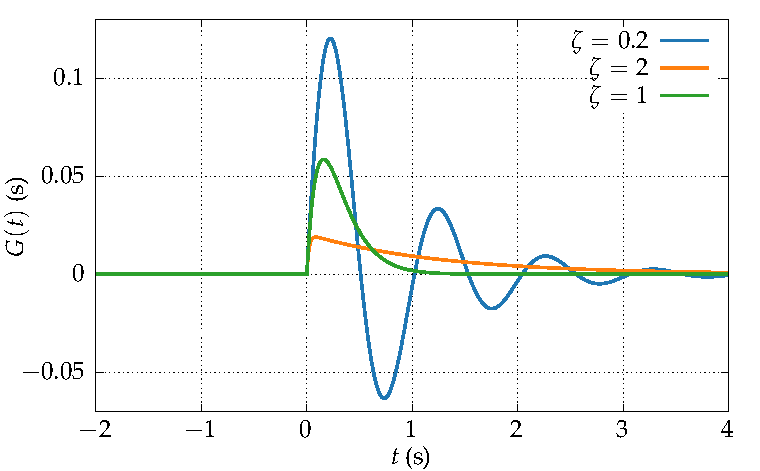
\includegraphics{gp_ho-green.pdf}
  \caption{Green's function of the damped harmonic oscillator in the underdamped,
    overdamped, and critical regimes for an undamped frequency $\omega_0=\unit{1}{\hertz}$.
    The explicit form of $G(t)$ is given in
  \cref{eq:green-underdamped,eq:green-overdamped,eq:green-critical}.}
  \label{fig:ho-green}
\end{figure}
%.........................................................................................
\subsubsection{Physical interpretation of the Green's function}
Let us discuss the physical interpretation of the Green's function. First we consider its
physical dimensions: $G$ is the solution of
\begin{equation}
  G''(t)+2\zeta\omega_0 G'(t)+\omega_0^2G(t)=\delta(t)\,.
\end{equation}
Firstly, the delta function has the inverse dimension of its argument. This can be seen,
for example, using the approximation of $\delta$ by a Gaussian kernel. So $\delta(t)$ is
an inverse time. Since $\omega_0$ is also an inverse time, the equation above implies that
$G(t)$ has the dimension of time. This is dimensionally consistent with
\cref{eq:green-underdamped}. Considering an arbitrary momentum $p$ (in
$\newton\usk\second$), then $\frac{p}{m}G(t)$ is the solution of \cref{eq:ode2-driven}
with the external force $F(t)=p\delta(t)$. So the Green's function is the response of the
oscillator when a momentum $p$ is instantly injected at $t=0$. This is why Green's functions
are also often called \emph{impulse response}, particularly in a signal theory or applied
physics context. With this interpretation in mind, the presence of the Heaviside function
$\theta(t)$ in~\cref{eq:green-underdamped} is not surprising: injecting momentum at $t=0$
only has an effect on the future, \ie for $t>0$. Such a Green's function is called
\emph{retarded} or \emph{causal}. One can observe through the derivation of $G(t)$ that
the $\theta(t)$ factor emerged from the condition $\Re(s_{\pm})<0$, which in turn comes
from $\zeta>0$. In the absence of damping (\ie for $\zeta=0$), one can show that the
definition of $G(t)$ becomes ambiguous, and can influence both future and past, which can
be counter-intuitive. The physical interpretation is that in the presence of damping, the
system loses energy and a clear direction of time is imposed. In the absence of damping,
time reversal becomes a symmetry of the system, and the Green's function can be
interpreted as the future response to an impulse, or the annihilation of a past movement.

Let us now discuss the interpretation of the frequency space Green's function, \ie
\begin{equation}
  \hat{G}(\omega)=\frac{1}{P(2\pi i\omega)}=\frac{1}{4\pi^2}
  \frac{1}{-\omega^2+2i\zeta\omega_0\omega+\omega_0^2}\,.
  \label{eq:ho-green-ft}
\end{equation}
In this form, the Green's function describes the response of the oscillator when driven at
a fixed frequency $\omega$. Indeed, for a force $A>0$ in Newtons, we can consider
\cref{eq:ode2-driven} where the external force is an elementary wave with amplitude $A$
and frequency $\omega$, \ie $F(t)=A\cos(2\pi\omega t)$. Then we know that a particular
solution of the equation is given by convoluting $F$ with the Green's function, leading to
\begin{equation}
  y_P(t)=\frac{1}{m}(F\ast G)(t)=\frac{A}{m}\intr{u}G(u)\cos[2\pi\omega(t-u)]\,.
\end{equation}
Using $\cos(x)=\Re(e^{ix})$, and the fact that $G$ is real, we obtain
\begin{equation}
  y_P(t)=\frac{A}{m}\Re\left[\intr{u}G(u)\,e^{2\pi i\omega(t-u)}\right]
  =\frac{A}{m}\Re[\hat{G}(\omega)\,e^{2\pi i\omega t}]\,.
\end{equation}
Let us now write $\hat{G}$ in the polar form
$\hat{G}(\omega)=R(\omega)\,e^{-i\phi(\omega)}$, which gives
\begin{equation}
  y_P(t)=\frac{AR(\omega)}{m}\cos[2\pi\omega t-\phi(\omega)]\,.
\end{equation}
We can make $R$ and $\phi$ more explicit, but before that let us physically interpret the
solution above. If the oscillator is driven by an external oscillation at frequency
$\omega$, the solution above tells us that the oscillator will also oscillate with
frequency $\omega$, although delayed by a phase $\phi(\omega)$. Additionally, this
oscillating movement has an amplitude proportional to $R(\omega)$. $R(\omega)$ is called
the \emph{frequency response} of the oscillator, and $\phi(\omega)$ is the \emph{phase
shift}. Let us compute explicitly these functions using~\cref{eq:ho-green-ft}. We start by
the frequency response
\begin{equation}
  R(\omega)=|\hat{G}(\omega)|=\frac{1}{4\pi^2}
  \frac{1}{\sqrt{(\omega_0^2-\omega^2)^2+4\zeta^2\omega_0^2\omega^2}}
  =\frac{1}{4\pi^2\omega_0^2}\bar{R}\left(\frac{\omega}{\omega_0}\right)\,,
\end{equation}
where $\bar{R}$ is the dimensionless function given by
\begin{equation}
  \bar{R}(\xi)=\frac{1}{\sqrt{(1-\xi^2)^2+4\zeta^2\xi^2}}\,.
  \label{eq:ho-response}
\end{equation}
For the phase shift, we first write
\begin{equation}
  \hat{G}(\omega)=\frac{R(\omega)^2}{4\pi^2}(-\omega^2-2i\zeta\omega_0\omega+\omega_0^2)\,,
\end{equation}
therefore $\phi(\omega)$ is such that
\begin{equation}
  \tan[\phi(\omega)]=\frac{2\zeta\omega_0\omega}{\omega_0^2-\omega^2}
  =\frac{2\zeta\xi}{1-\xi^2}\,,
  \label{eq:ho-phase}
\end{equation}
where $\xi=\frac{\omega}{\omega_0}$.
\begin{figure}[p]
  \centering
  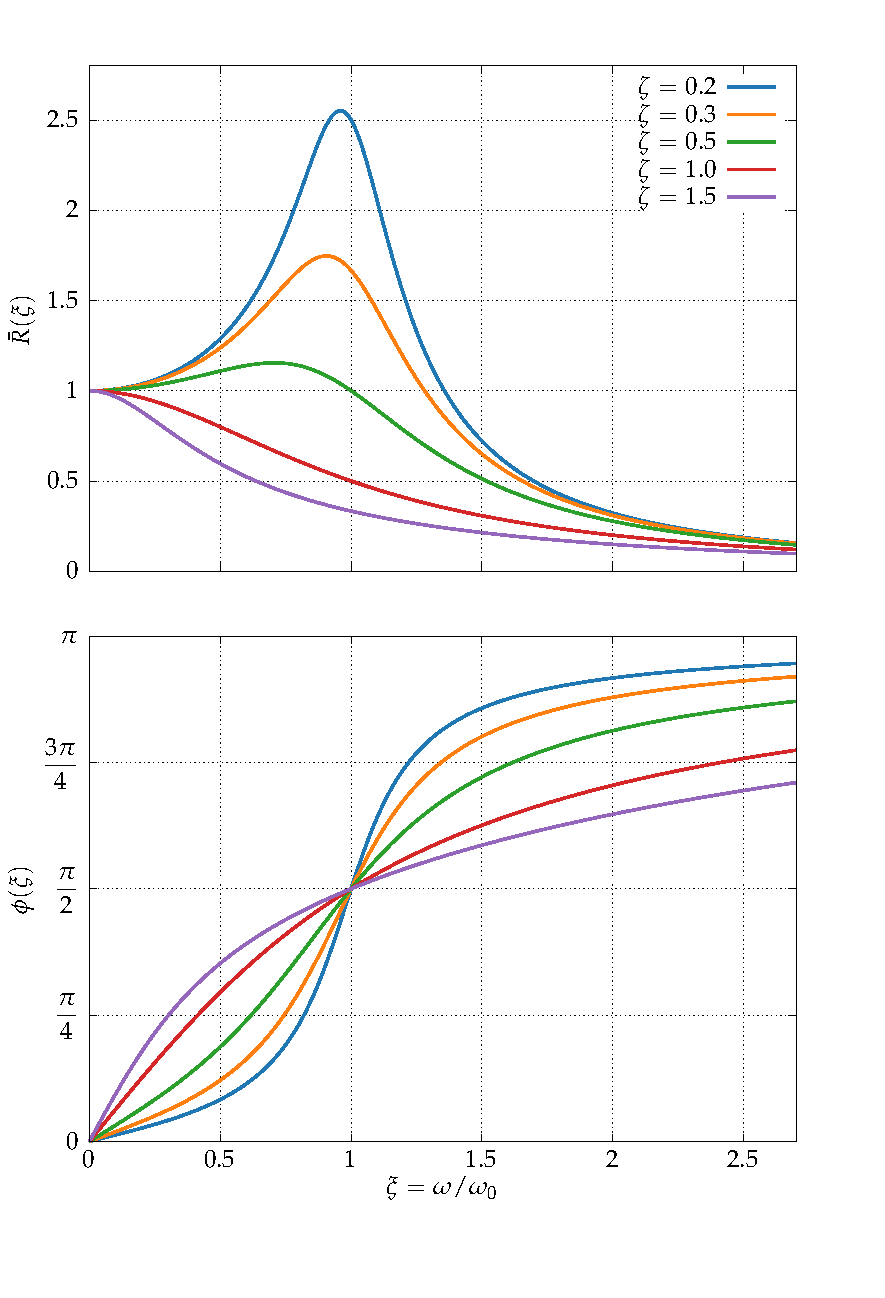
\includegraphics{gp_resonance.pdf}
  \caption{Frequency response (upper pane) and phase shift (lower pane) of the driven
    harmonic oscillator as a function of the frequency ratio $\xi=\frac{\omega}{\omega_0}$,
    where $\omega_0$ is the undamped oscillator frequency. Both functions are defined
    in~\cref{eq:ho-response,eq:ho-phase}, and the phase shift was defined in the
  interval~$[0,\pi)$.}
  \label{fig:resonance}
\end{figure}

The frequency response and phase shift are represented in~\cref{fig:resonance} for various
values of the damping ratio $\zeta$. In the underdamped $\zeta<1$ regime, we clearly
observe that for frequencies around the undamped frequency $\omega_0$, the amplitude of
oscillations is amplified. This is the well-known \emph{resonance} phenomenon which is a
characteristic feature of the driven harmonic oscillator. Regarding the phase shift in the
resonant regime, at frequencies much lower than $\omega_0$, $\phi(\omega)$ is close to
$0$, and at frequencies much higher than $\omega_0$, $\phi(\omega)$ is close to $\pi$.
This can be physically interpreted in the following way: $\omega_0$ is a characteristic
frequency of the oscillator, as it is determined by its mass and spring constant. If the
driver oscillates much slower than this frequency, then the oscillator is able to follow
this movement with a negligible reaction time and is in phase with the driver. However,
if the driver oscillates much faster than $\omega_0$, the reaction time of the oscillator
is too slow to be synchronised, and it is completely out of phase with the driver.

\vfill\pagebreak
% !TEX root = ../waves.tex
%%%%%%%%%%%%%%%%%%%%%%%%%%%%%%%%%%%%%%%%%%%%%%%%%%%%%%%%%%%%%%%%%%%%%%%%%%%%%%%%%%%%%%%%%%
\section{Exercises}
\begin{ExerciseList}
  %---------------------------------------------------------------------------------------
  \Exercise[label=ode-hom]
  Solve the homogeneous differential equations below.
  \Question $y''+2y'+2=0$
  \Question $y^{(3)}-3y''+7y'-5=0$
  \Question $y^{(3)}-6y''+12y'-8=0$
  %---------------------------------------------------------------------------------------
  \Exercise[label=ode-rev]
  For all cases below, find a differential equation for which $y$ is a solution.
  \Question $y(t)=\cos(3t)$
  \Question $y(t)=\cos(2t)-\sin(t)$
  \Question $y(t)=(1+2t+3t^2)e^{-t}+\cos(2t)$
  %---------------------------------------------------------------------------------------
  \Exercise[label=ode4]
  We consider the following homogeneous order $4$ ordinary differential equation:
  \begin{equation}
    y^{(4)}+2y^{(2)}+(1-a^2)y=0\,,
    \label{eq:ode4}
  \end{equation}
  where $a$ is a positive real number.
  \Question Solve~\cref{eq:ode4} in the following cases:
  \subQuestion $a<1$, show that $y$ is an oscillating solution according to two frequencies.
  \subQuestion $a>1$, show that $y$ is oscillating with one frequency, and exponentially varying.
  \subQuestion $a=1$.
  %---------------------------------------------------------------------------------------
  \Exercise[label=airy]
  We consider the Airy differential equation
  \begin{equation}
    y''(x)-xy(x)=0
  \end{equation}
  \Question Show that the Fourier transform $\hat{y}$ satisfies the differential equation
  \begin{equation}
    \hat{y}'(\omega)=i8\pi^3\omega\,\hat{y}(\omega)\,.
  \end{equation}
  \Question Show that there exists a constant $C$ such that $\hat{y}(\omega)=C\,e^{i8\pi^3\frac{\omega^3}{3}}$.
  \Question Show that $y$ is given by $y(x)=C\,\mathrm{Ai}(x)$
  where $\mathrm{Ai}$ is the \emph{Airy function} given by
  \begin{equation}
    \mathrm{Ai}(x)=\frac{1}{\pi}\int_{0}^{+\infty}\diff t\,\cos\left(\frac{t^3}{3}+xt\right)\,.
  \end{equation}
  %---------------------------------------------------------------------------------------
  \Exercise[label=green] We consider once more the driven harmonic oscillator equation
  (\cf\cref{eq:ode2-driven})
  \begin{equation}
    x''+2\zeta\omega_0x'+\omega_0^2x=\frac{F}{m}\,.
  \end{equation}
  \Question Check explicitly that~\cref{eq:green-underdamped} is a Green's function of the
  equation above, \ie show that
  \begin{equation}
    G''(t)+2\zeta\omega_0G'(t)+\omega_0^2G(t)=\delta(t)\,,
  \end{equation}
  in the sense of distributions.
  \Question Compute the green function in the overdamped ($\zeta=1$) and critical
  ($\zeta=1$) regimes.
\end{ExerciseList}

\shipoutAnswer
\end{document}
